\documentclass{classes/fiboThesis}
\usepackage{tabularx}
\usepackage{graphicx}
\usepackage{adjustbox}
\usepackage{lscape}

\begin{document}
	\title{Goggle : People Video Analytics and Deep Learning Platform}
	\titleTH{Goggle แพลตฟอร์มการเรียนรู้เชิงลึกและระบบวิเคราะห์การกระทำของมนุษย์}

	\author{นายปฐมพงศ์ สินธุ์งาม}
	\authorTwo{นายศุภกร เบญจวิกรัย}
	\authorThree{นายอุกฤษฎ์ เลิศวรรณาการ}

	\majoradvisor{ดร.วราสิณี ฉายแสงมงคล}
	\committeeOne{ดร.วราสิณี ฉายแสงมงคล}
	\committeeTwo{อ.บวรศักดิ์ สกุลเกื้อกูลสุข}
	\committeeThree{ดร.บุญฑริกา เกษมสันติธรรม}

	\academicyearTH{2562}	

	\maketitle
	\frontmatter
	\maketitleinner
	\makeapproval
	% ************************** Thesis Abstract **********************************
\begin{abstract}
งานวิทยานิพนธ์นี้เป็นงานที่เกี่ยวกับการออกแบบและจัดทำแพลตฟอร์มหุ่นยนต์ฮิวมานอยด์ด้วยเครื่องพิมพ์สามมิติ
โดยใช้ชื่อว่า หุ่นยนต์ฮิวมานอยด์ UTHAI และจุดประสงค์เพื่อให้นักวิจัยท่านอื่นสามารถนำไปพัฒนาต่อได้ง่าย
ภาพรวมของวิทยานิพนธ์นี้จะแบ่งออกเป็นทั้งหมดสามส่วน คือ ส่วนแรกเป็นส่วนของการออกแบบและจัดสร้างส่วนโครงสร้างของหุ่นยนต์ฮิวมานอยด์
ส่วนที่สองเป็นส่วนของการพัฒนาโปรแกรมที่ใช้ในระบบด้วย ROS และส่วนสุดท้ายเป็นส่วนที่ออกแบบระบบพื้นฐานสำหรับการพัฒนาหุ่นยนต์ฮิวมานอยด์
รวมไปถึงมีเอกสาร คู่มือที่อยู่ในรูปแบบออนไลน์
\vfill
\paragraph*{คำสำคัญ :} แพลตฟอร์มหุ่นยนต์ฮิวมานอยด์ / ระบบพื้นฐานหุ่นยนต์ / ROS / เครื่องพิมพ์สามมิติ 
\vfill
\end{abstract}
	% ************************** Thesis Acknowledgements **************************
% \majoradvisor{นายธนัชชา ชูพจน์เจริญ}
% \coadvisor{รศ.ดร.ชิต เหล่าวัฒนา}
% \committeeOne{ดร.อาบทิพย์ ธีรวงศ์กิจ}
% \committeeTwo{ดร.ปิติวุฒญ์ ธีรกิตติกุล}
% \committeeThree{ดร.สุภชัย วงศ์บุณย์ยง}
\begin{acknowledgements}
ขอขอบพระคุณ ดร.วราสิณี ฉายแสงมงคล อาจารย์ที่ปรึกษาวิทยานิพนธ์หลัก
ที่ได้สละเวลามาให้คำปรึกษา ชี้แนะแนวทาง ให้ความรู้ในด้านต่างๆ ที่จำเป็นต่องานวิจัย 
รวมถึงการให้การสนับสนุนในเรื่องอุปกรณ์ในการทำวิจัย ช่วยตรวจและแก้ไขวิทยานิพนธ์ให้เป็นไปอย่างสมบูรณ์
ตลอดจนกรุณาให้เกียรติเป็นประธานกรรมการสอบวิทยานิพนธ์

ขอขอบพระคุณอาจารย์อาจารย์ บวรศักดิ์ สกุลเกื้อกูลสุข ที่กรุณาให้เกียรติเป็นกรรมการสอบวิทยานิพนธ์ 
ให้คำแนะนำที่เป็นประโยชน์ต่อการวิจัย และการแก้ไขปรับปรุงงานวิจัย ตลอดจนตรวจแก้วิทยานิพนธ์ให้ดำเนินไปอย่างสมบูรณ์

ขอขอบพระคุณอาจารย์ ดร.บุญฑริกา เกษมสันติธรรม ที่กรุณาให้เกียรติเป็นกรรมการสอบวิทยานิพนธ์ 
ให้คำแนะนำที่เป็นประโยชน์ต่อการวิจัย และการแก้ไขปรับปรุงงานวิจัย ตลอดจนตรวจแก้วิทยานิพนธ์ให้ดำเนินไปอย่างสมบูรณ์

ขอขอบพระคุณคณาจารย์ และบุคลากรในสถาบันวิทยาการหุ่นยนต์ภาคสนามทุกท่าน
ที่ได้ให้คำปรึกษาและช่วยเหลือด้านสถานที่พร้อมทั้งสิ่งอำนวยความสะดวกต่างๆ ในระหว่างการทำวิทยานิพนธ์

ขอขอบคุณนักศึกษาปริญญาตรี สถาบันวิทยาการหุ่นยนต์ภาคสนามทุกท่าน
ที่ได้ให้คำแนะนำ ถามไถ่ และเป็นกำลังใจมาโดยตลอด

และสุดท้ายนี้ ขอน้อมรำลึกถึงพระคุณบิดา มารดา และครอบครัว ที่ส่งเสริมให้กำลังใจ
และให้การสนับสนุนในเรื่องต่างๆ จนกระทั่งข้าพเจ้าประสบความสำเร็จในการศึกษา
\end{acknowledgements}

	\tableofcontents
	\listoffigures
	\listoftables
	%% ***************************** Thesis Symbols ********************************
\begin{symbols}
    \noindent
    \begin{tabular*}{\textwidth}{@{}p{0.18\textwidth}p{0.8\textwidth}@{}}
        {$\theta$} & {เซต้า} \\
        {$d$} & {distance} \\
        {kg} & {Kilogram} \\
        {m$^{2}$} & {Square Metre} \\
    \end{tabular*}
\end{symbols}
	% ************************** Thesis Abbreviations **************************
\begin{abbreviations}
    \noindent
    \begin{tabular*}{\textwidth}{@{}p{0.3\textwidth}p{0.8\textwidth}@{}}
        {AVA} & {Atomic Visual Actions} \\
        {Machine learning} & {การเรียนรู้ของเครื่อง} \\
        {Artificial intelligence} & {ปัญญาประดิษฐ์} \\
        {Label} & {คำอธิบายที่บ่งบอกถึงคุณลักษณะของสิ่งที่เราสนใจ} \\
        {Labeling} & {การสร้างคำอธิบายคุณลักษณะ} \\
        {Action recognition} & {การจดจดจำการกระทำ} \\
        {Video labeling} & {การสร้างคำอธิบายคุณลักษณะภายในวิดิโอ} \\
        {Video analytics} & {การวิเคราะห์ผลวิดิโอ} \\
	{Video analytics platform} & {ระบบปฎิบัติการสำหรับช่วยวิเคราะห์ผลวิดิโอ} \\
        {Goggle labeling tool} & {เครื่องมือของโปรเจค Goggle สำหรับช่วยสร้างคำอธิบายที่บ่งบอกถึงคุณลักษณะของสิ่งที่เราสนใจ} \\
        {Uniform label distribution} & {การที่มีจำนวนตัวอย่างภายในคลาสเท่ากันทุกคลาส} \\
        {KMUTT} & {King Mongkut's University of Technology Thonburi} \\
        {Liews} & {วุฒิภัทร โชคอนันตทรัพย์} \\
        {$\theta$} & {เซต้า}
    \end{tabular*}
\end{abbreviations}

	
	\mainmatter
	\chapter{บทนำ}
%%%%%%%%%%%%%%%%%%%%%%%%%%%%%%%%%%%%%%%%%%%%%%%%%%%%%%%%%%%%%%%%%%%%%%%%%%%%%%%
\section{ที่มาและความสำคัญ}
บริษัท เพอเซ็ปทรา ดำเนินธุรกิจเกี่ยวกับด้าน artificial intelligence service โดยลูกค้านั้นมีความต้องการที่จะให้ทางบริษัทสร้าง artificial intelligence เพื่อนำไปใช้งานหรือแก้ปัญหาที่ต่างกันออกไป ทำให้การ artificial intelligence เพื่อตอบสนองความต้องการของลูกค้าเหล่านั้นต้องมีชุดข้อมูลที่เหมาะสมกับปัญหานั้นๆ เช่น ร้านขายของแห่งหนึ่งต้องการรู้ว่าในแต่ละวันมีลูกค้าเดินเข้าร้านกี่คน เป็นผู้ชายกี่คน เป็นผู้หญิงกี่คน เป็นต้น ซึ่งการจะได้ข้อมูลที่เหมาะสมกับงานนั้น ต้องใช้มนุษย์ในการสร้างขึ้นมาโดยการเก็บข้อมูลวิดีโอ และสร้าง label สำหรับใช้ในการสร้างโมเดล machine learning ด้วยตัวเอง ถ้าหากมีวิดีโอเป็นจำนวนมาก การที่จะใช้มนุษย์ในการสร้าง label นั้นอาจจะต้องใช้มนุษย์เป็นจำนวนมาก หรือ ก่อให้เกิดภาระแก่มนุษย์ อีกทั้งการสร้าง label 

นั้นเป็นงานที่ลำบาก และน่าเบื่อ
ทางคณะผู้วิจัยจึงมีความต้องการที่จะออกแบบ และพัฒนา video analytics platform ที่มีเครื่องมือในการสร้าง label สำหรับวิดีโอ เพื่อช่วยแบ่งเบาภาระของผู้พัฒนาในการสร้าง label เพื่อนำไปสร้างโมเดล machine learning สำหรับใช้แก้ปัญหาที่ลูกค้าต้องการ โดยโครงการสหกิจนี้เน้นศึกษาการวิเคราะห์และจดจำการกระทำของมนุษย์จากภาพเคลื่อนไหวเป็นหลัก

%%%%%%%%%%%%%%%%%%%%%%%%%%%%%%%%%%%%%%%%%%%%%%%%%%%%%%%%%%%%%%%%%%%%%%%%%%%%%%%
\section{วัตถุประสงค์}
\begin{enumerate}
	\setlength\itemsep{-0.25em}
	\item เพื่อออกแบบ และ สร้างระบบที่สามารถตรวจจับมนุษย์ และจดจำการกระทำพื้นฐานของมนุษย์ภายในสำนักงาน ประกอบด้วย ยืน นั่ง ใช้คอมพิวเตอร์ เล่นโทรศัพท์ เดิน กินข้าว โดยใช้ปัญญาประดิษฐ์มาประมวลผลกับวิดีโอ
	\item เพื่อพัฒนาเครื่องมือในการทำ video labeling ในการสร้างข้อมูลที่ใช้สร้างโมเดลจากวิดีโอ ให้สามารถทำได้ง่าย และ มีประสิทธิภาพที่สูงกว่าเครื่องมือตัวอื่นในปัจจุบัน
\end{enumerate}

%%%%%%%%%%%%%%%%%%%%%%%%%%%%%%%%%%%%%%%%%%%%%%%%%%%%%%%%%%%%%%%%%%%%%%%%%%%%%%%

\section{ประโยชน์ที่คาดว่าจะได้รับ}
\begin{enumerate}
	\setlength\itemsep{-0.25em}
	\item พัฒนาเครื่องมือในการทำ labeling โดยมี artificial intelligence เข้ามาช่วย ที่สามารถสร้าง label ที่สามารถนำไปใช้สร้างโมเดล machine learning ได้
	\item พัฒนาต้นแบบของ video analytics platform ที่สามารถรับวิดีโอเข้ามาในระบบแล้วสร้างรายงานเกี่ยวกับกิจกรรมของมนุษย์ในวิดีโอได้
	\item สร้างและทดสอบโมเดลสำหรับทำ action recognition อย่างน้อย 2 โมเดล
\end{enumerate}
\clearpage

%%%%%%%%%%%%%%%%%%%%%%%%%%%%%%%%%%%%%%%%%%%%%%%%%%%%%%%%%%%%%%%%%%%%%%%%%%%%%%%
\section{ขอบเขตการดำเนินงาน}
\begin{enumerate}
	\setlength\itemsep{-0.25em}
	\item Labeling tool สามารถตัดวิดิโอเฉพาะในช่วงเวลาที่มีมนุษย์อยู่ได้อัตโนมัติ
	\item Labeling tool สามารถระบุตำแหน่งได้ว่ามนุษย์แต่ละคนในวิดีโออยู่ตรงส่วนใดของวิดีโอและสามารถระบุการกระทำของมนุษย์ในวิดีโอได้ ประกอบด้วยกระทำได้แก่ ยืน นั่ง ใช้คอมพิวเตอร์ เล่นโทรศัพท์ เดิน กินข้าว 
	\item Label ผลลัพธ์ที่ได้จาก labeling tool ต้องสามารถนำไปใช้ในการสร้างโมเดลต่อได้
	\item พัฒนา Labeling tool ด้วยภาษา Python
	\item พัฒนา Labeling tool ที่สามารถให้มนุษย์ทำงานแก้ไขได้ เมื่อระบบอัตโนมัติทำงานผิดพลาด
	\item สร้างโมเดลสำหรับการทำ action recognition อย่างน้อย 2 โมเดลที่สามารถระบุการกระทำของมนุษย์ตามที่กำหนดไว้ได้ เพื่อนำไปใช้ใน video analytics platform
	\item Video analytics platform ต้องสามารถนำวิดีโอมาวิเคราะห์ข้อมูลการกระทำและตำแหน่งของมนุษย์แต่ละคนได้ แล้วนำข้อมูลเหล่านั้นไปสร้างรายงานออกมาได้
	\item ความละเอียดอย่างต่ำของวิดีโอต้องมากกว่า 640 x 480 (ยาว x สูง)
	\item วิดีโอจะต้องมีเฟรมเรท (fps) อย่างต่ำ 24 fps
\end{enumerate}

%%%%%%%%%%%%%%%%%%%%%%%%%%%%%%%%%%%%%%%%%%%%%%%%%%%%%%%%%%%%%%%%%%%%%%%%%%%%%%%
\section{ภาพรวมของระบบและขั้นตอนการดำเนินงาน}
งานวิจัยนี้การดำเนินงานวิจัยถูกแบ่งออกเป็นสองส่วน คือ ส่วนที่หนึ่งส่วนเครื่องมือสำหรับการเตรียมชุดข้อมูล (dataset) เป็นส่วนที่ทำเครื่องมือสำหรับช่วยผู้พัฒนาในการสร้างชุดข้อมูล และส่วนที่สองนำชุดข้อมูลไปสร้างโมเดล
\subsection*{ศึกษาค้นคว้าเอกสารและงานวิจัยที่เกี่ยวข้อง}
\begin{enumerate}\setlength\itemsep{-0.25em}
	\item ศึกษาเกี่ยวกับการวิเคราะห์ผลวิดิโอ (video analytics)
	\item ศึกษาเกี่ยวกับชุดข้อมูลสำหรับการวิเคราะห์ผลวิดิโอ
	\item ศึกษาเกี่ยวกับโมเดลใช้ในการวิเคราะห์ผลวิดิโอ
	\item ศึกษาเครื่องมือที่ใช้สำหรับช่วยสร้างชุดข้อมูล
\end{enumerate}
\subsection*{ส่วนเครื่องมือสำหรับการเตรียมชุดข้อมูล}
\begin{enumerate}\setlength\itemsep{-0.25em}
	\item ออกแบบหน้าต่างของแอพพลิเคชั่น
	\item สร้างระบบของแอพพลิเคชั่น
	\item ทดสอบการทำงานของแอพพลิเคชั่น
\end{enumerate}
\subsection*{ส่วนนำชุดข้อมูลไปสร้างโมเดล}
\begin{enumerate}\setlength\itemsep{-0.25em}
	\item สร้างชุดข้อมูลสำหรับสร้างโมเดล
	\item สร้างโมเดลสำหรับการทำนายการกระทำของมนุษย์
	\item ทดสอบการทำงานของโมเดล
\end{enumerate}
\clearpage
%%%%%%%%%%%%%%%%%%%%%%%%%%%%%%%%%%%%%%%%%%%%%%%%%%%%%%%%%%%%%%%%%%%%%%%%%%%%%%%
\section{Gantt chart}แผนการทำงานของคณะวิจัยจะแบ่งออกเป็น 3 ช่วง ซึ่งในแต่ละช่วงจะมี task ดังนี้
\begin{enumerate}
	\item Phase 1 :  ศึกษาข้อมูลเกี่ยวกับการทำวิเคราะห์วิดีโอและเครื่องมือที่ใช้ในการทำโครงการวิจัย
		\begin{enumerate}\setlength\itemsep{-0.25em}
			\item task 1 	ศึกษา และ ทดลองใช้เทคนิคที่เกี่ยวข้องกับการวิเคราะห์วิดีโอ
			\item task2	รวบรวมชุดข้อมูลสำหรับการทำ human action recognition
		\end{enumerate}
	\item Phase 2 :  สร้างและออกแบบแอพพลิเคชั่นโดยจะประกอบด้วยงานในส่วนหลักๆ คือ
		\begin{enumerate}\setlength\itemsep{-0.25em}
			\item task3	โมเดลสำหรับวิเคราะห์ผลการกระทำของมนุษย์
			\item task4	หน้าต่าง UI
		\end{enumerate}
	\item Phase 3 : ปรับปรุงและแก้ไขปัญหา ทำให้แอพพลเคชั่นสามารถนำไปใช้งานได้จริง
\end{enumerate}

%%%%%%%%%%%%%%%%%%%%%%%%%%%%%%%%%%%%%%%%%%%%%%%%%%%%%%%%%%%%%%%%%%%%%%%%%%%%%%%
\section{Milestones}จะมีการกำหนด milestones ทั้งหมด 3 ครั้ง คือ
\begin{enumerate}
	\item Milestone  1  วันที่ 12  มิถุนายน  2562
		\begin{enumerate}\setlength\itemsep{-0.25em}
			\item ศึกษางานวิจัยที่เกี่ยวข้องกับการวิเคราะห์วิดีโอต่าง ๆ  ได้แก่ Youtube-8M , Moment in time , AVA
		\end{enumerate}
	\item Milestone  2  วันที่ 14  สิงหาคม 2562
		\begin{enumerate}\setlength\itemsep{-0.25em}
			\item สร้างหน้าต่าง UI ครบสมบูรณ์
			\item ความคืบหน้าของโมเดลมากกว่า 50 \%-symbol
			\item ฟังก์ชั่นการทำงานของแอพพลิเคชั่นสามารถทำงานได้มากกว่า 50 \%-symbol
		\end{enumerate}
	\item Milestone  3  วันที่ 15  ตุลาคม 2562
		\begin{enumerate}\setlength\itemsep{-0.25em}
			\item แอพพลิเคชั่นสามารถทำงานได้ครบกระบวนการ
			\item ได้โมเดลสามารถทำนายการกระทำของมนุษย์ได้
		\end{enumerate}
\end{enumerate}




	% ************************** Thesis Chapter2 **********************************
\clearpage
\chapter{ทฤษฎี/การวิจัยที่เกี่ยวข้อง}
การวิเคราะห์วิดีโอในปัจจุบันนั้นมีวิธีและเทคนิคมากมาย ผู้วิจัยจึงต้องศึกษาองค์ความรู้และงานวิจัยที่เกี่ยวข้องกับวัตถุประสงค์ของงาน 
เพื่อศึกษาและใช้เป็นแนวทางในการประยุกต์สำหรับสร้างเครื่องมือสำหรับกำกับข้อมูลด้วยปัญญาประดิษฐ์ และโมเดลปัญญาประดิษฐ์สำหรับการจำแนกการกระทำของมนุษย์ 
ซึ่งหัวข้อที่ผู้วิจัยได้ไปศึกษามา มีดังต่อไปนี้
\begin{enumerate}
	\setlength\itemsep{-0.25em}
	\item การวิเคราะห์ผลวิดีโอ
	\begin{enumerate}	
		\item การตรวจจับวัตถุ (object detection)
		\item การทำนายตำแหน่งถัดไปของวัตถุ (object tracker)
		\item การระบุตัวตนของบุคคล (person re-identification)
		\item การจำแนกการกระทำ (action classification)
	\end{enumerate}
	\setlength\itemsep{-0.25em}
	\item เครื่องมือสำหรับการวิเคราะห์ผลวิดีโอ
	\begin{enumerate}	
		\item โมเดลปัญญาประดิษฐ์สำหรับจำแนกการกระทำมนุษย์
		\item เครื่องมือสำหรับกำกับชุดข้อมูล (labeling tool)
	\end{enumerate}
	\item ทฤษฎีที่เกี่ยวข้อง
	\begin{enumerate}	
		\item Optical flow
	\end{enumerate}
\end{enumerate}

\section{การวิเคราะห์ผลวิดีโอ}
ในส่วนของงานวิจัยสิ่งที่เราให้ความสนใจ คือ ข้อมูลการกระทำของมนุษย์แต่ละคนภายในวิดีโอ  ซึ่งเพื่อที่เราจะได้ผลลัพธ์ที่มีประสิทธิภาพออกมาเป็นข้อมูลของสิ่งที่เราสนใจและสามารถนำไปใช้ต่อได้ เราจึงจำเป็นจะต้องใช้การวิเคราะห์ผลวิดีโอเพื่อที่จะสกัดสิ่งที่เราสนใจออกมาจากวิด๊โอ ซึ่งการวิเคราะห์ผลวิดีโอมีหลากหลายกระบวนการในการทำ จะทำทีละขั้นตอน โดยในแต่ละกระบวนการจะมีจุดประสงค์ของการทำและผลลัพธ์หลังการทำที่แตกต่างกัน ในหัวข้อนี้จะมาอธิบายถึงกระบวนการในการวิเคราะห์ผลของวิดิโอและผลลัพธ์ของการทำกระบวนการนั้น

\subsubsection*{2.1.1 การตรวจจับวัตถุ}
การตรวจจับวัตถุเป็นสิ่งที่สำคัญเป็นอันดับต้นๆของการวิเคราะห์ผลของวิดีโอ คือ การตรวจจับวัตถุ กล่าวคือกระบวนการที่ผู้วิจัยจะต้องทำคือระบุสิ่งที่สนใจว่าคืออะไร อยู่ตำแหน่งใด ซึ่งในปัจจุบันการทำการตรวจจับวัตถุมักนำ Machine learning model มาใช้เพื่อช่วยตรวจจับวัตถุที่เราสนใจ ซึ่ง Machine learning model ที่เราเลือกใช้คือ YOLO v3 โดยเหตุผลที่เราเลือกใช้ Machine learning model YOLO v3 จะถูกกล่าวไว้อยู่ในหัวข้อ Machine learning model ในหัวข้อถัดไป
\par
YOLO v3 เป็น Machine learning model ที่ในปัจจุบันนิยมนำมาใช้ตรวจจับวัตถุในงานวิเคราะห์ผลของวิดีโอ เนื่องจากสามารถตรวจจับวัตถุได้แบบเรียลไทม์และมีความแม่นยำ โดยหลักการของ YOLO v3 คือ นำรูปภาพที่ต้องการตรวจจับตำแหน่งของวัตถุผ่าน neural network โดยโครงข่ายจะแบ่งรูปภาพเป็นพื้นที่ และ จะทำนายกรอบสี่เหลี่ยมพร้อมกับทำนายความน่าจะเป็นของแต่ละหมวดหมู่ในแต่ละพื้นที่ สุดท้ายจะเลือกกรอบสี่เหลี่ยมและหมวดหมู่ที่มีค่าคะแนนความน่าจะเป็นมากที่สุด

\subsubsection*{2.1.2 การทำนายตำแหน่งถัดไปของวัตถุ (Tracking)}
การติดตามการเคลื่อนไหวของวัตถุ\textsuperscript{\cite{danelljan2014accurate}} คือระบบที่ใช้สำหรับการติดตามการเคลื่อนไหวของวัตถุที่สนใจที่อยู่ในรูปภาพ 
โดยใช้การคำนวณทางคณิตศาสตร์ และการประมวลผลภาพ (image processing) ทำให้การประมวลผลนั้นเร็วกว่าการใช้โมเดลปัญญาประดิษฐ์ ซึ่งอัลกอริทึมติดตามการเคลื่อนไหวที่นิยมใช้มีสองอัลกอริทึม
คือ correlation filter และ kalman filter ซึ่งหลักการของทั้งสองอัลกอริทึมนั้นจะแตกต่างกันโดยที่ correlation filter นั้นจะใช้พิกเซลของวัตถุในการคำนวณตำแหน่งถัดไปของวัตถุ 
และ kalman filter จะใช้ข้อมูลการเคลื่อนไหวในการคำนวณตำแหน่งถัดไปของวัตถุ ซึ่งจากการศึกษาในบทความ "Object Tracking using Correlation,
Kalman Filterand Fast Means Shift Algorithms"\textsuperscript{\cite{ali2006object}} kalman filter มีประสิทธิภาพที่สูงนั้นจะขึ้นอยู่กับข้อมูลที่ได้จากการวัด (measurement)
และความซับซ้อนในการเคลื่อนไหวของวัตถุ ในขณะที่ correlation นั้นมีประสิทธิภาพที่ด้อยกว่า kalman filter เพียงเล็กน้อยและสามารถติดตามการเคลื่อนไหวที่ซับซ้อนของวัตถุได้ดีกว่า 
(การเคลื่อนไหวที่ซับซ้อนหมายถึง การเคลื่อนไหวที่เกิดการเปลี่ยนทิศทางฉับพลันบ่อย) ผู้วิจัยจึงตัดสินใจเลือกใช้ correlation filter ในงานครั้งนี้
\begin{figure}[!ht]
	\centering
	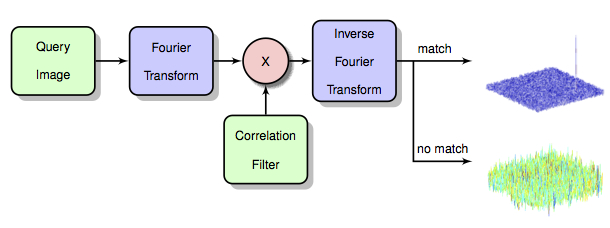
\includegraphics[width=1\textwidth]{chapter2/images/track-concept.png}
		\caption[แนวคิดของระบบติดตามการเคลื่อนไหวของวัตถุ]{แนวคิดของระบบติดตามการเคลื่อนไหวของวัตถุ\textsuperscript{\cite{correlation_filter}}}
    	\label{fig:Track_concept}
\end{figure}

จากรูปที่ \ref{fig:Track_concept} เป็นหลักการในการติดตามการเคลื่อนไหวของวัตถุแบบ correlation filter โดยการนำรูปมาผ่านกระบวนการแปลงฟูรีเยร์ (fourier transform)
และนำมาคูณกับ correlation filter ซึ่งเป็นตัวกรองที่ใช้สำหรับการหาความสัมพันธ์กับวัตถุในภาพ จากนั้นทำการแปลงฟูรีเยร์ผกผัน (inverse fourier transform) 
เพื่อตรวจสอบว่าวัตถุในภาพนั้นอยู่ที่ตำแหน่งใด โดยมีการคำนวณเริ่มจากการหา correlation filter ที่ดีที่สุดโดยใช้วิธีลดผลรวมของข้อผิดพลาดกำลังสองให้น้อยที่สุดดังนี้

\begin{equation}
\epsilon = \left \| \sum_{l = 1}^{d} h^{l} \star f^{l} - g \right \|^2 + \lambda \sum_{l = 1}^{d}\left \| h^{l} \right \|^2
\end{equation}
โดยที่
\begin{conditions}
 \epsilon     	&   ค่าความคลาดเคลื่อน 							\\
 d      		&  จำนวนมิติของผังคุณลักษณะของภาพ  \\   
 h 			&  correlation filter								\\
\star 			&  circular correlation							\\
 f			&  พื้นที่สี่เหลี่ยมของวัตถุที่สนใจที่ได้จากการทำผังคุณลักษณะ	\\
 g			&  ผลลัพธ์ correlation ที่ต้องการของ f					\\
 \lambda   		&  regularization term
\end{conditions}

เมื่อพิจารณาจากรูปภาพเดียวในกรณีที่เวลา ($t$) เท่ากับ 1 จะสามารถจัดรูปสมการด้านบนได้ดังนี้ 

\begin{equation}
H^{l} = \frac{\bar{G}F^{l}}{\sum_{k=1}^{d}\bar{F^{k}}F^{k} + \lambda}
\end{equation}
\begin{equation}
H_{t}^{l} = \frac{A_{t}^{l}}{B_{t}}					
\end{equation}					
\begin{equation}
A_{t}^{l} = (1-\eta )A_{t-1}^{l} + \eta \bar{G_{t}}F_{t}^{l}
\end{equation}
\begin{equation}
B_{t} = (1-\eta )B_{t-1} + \eta \sum_{k=1}^{d}\bar{F_{t}^{k}}F_{t}^{k}
\end{equation}
\clearpage
\noindent
โดยที่
\begin{conditions}
 H 		     	&   correlation filter								\\
 \eta      		&  อัตราการเรียนรู้						 		\\   
 \bar{G} 		&  g ที่ผ่านการทำ complex conjugation					\\
 F			&  พื้นที่สี่เหลี่ยมของวัตถุที่สนใจที่ได้จากการทำผังคุณลักษณะ	\\
 \bar{F}		&   f ที่ผ่านการทำ complex conjugation					\\
 t 	  		&  เวลา
\end{conditions}
จากสมการที่ได้มาจะสามารถทำให้หาตำแหน่งต่อไปของวัตถุที่สนใจได้ด้วยสมการต่อไปนี้
\begin{equation}
y = F^{-1}\left \{ \frac{\sum_{l = 1}^{d} \bar{A^{l}}Z^{l}}{B + \lambda} \right \}
\end{equation}
โดยที่
\begin{conditions}
 y 		     	&   correlation score										\\
 F^{-1}    		&  การแปลงฟูรีเยร์ผกผันแบบไม่ต่อเนื่อง (inverse discrete fourier transform)						\\   	
 \bar{A}^{l} 	&  $A^{l}$ ที่ผ่านการทำ complex conjugation				\\
 Z	 		&  พื้นที่สี่เหลี่ยมของวัตถุที่สนใจที่ได้จากการหาผังคุณลักษณะของภาพใหม่	
\end{conditions}
โดยค่าของ $y$ ที่ได้ออกมาจะทำให้รู้ถึงตำแหน่งของวัตถุที่สนใจได้ ณ ตำแหน่งที่ $y$ มีค่าสูงสุด

\subsubsection*{2.1.3 การระบุตัวตนของบุคคล (ReID)}
ระบบระบุตัวตนของบุคคล\textsuperscript{\cite{luo2019alignedreid++}}\textsuperscript{\cite{zhang2017alignedreid}} คือการระบุตัวตนของบุคคลภายในวิดีโอหรือระหว่างสองภาพ สามารถนำมาประยุกต์ใช้ในด้านของการรักษาความปลอดภัย 
หรือการตามหาบุคคล ซึ่งการระบุตัวตนของบุคคลนั้นเป็นปัญหาที่ท้าทาย เนื่องจากคุณลักษณะทั่วไปของบุคคลในภาพไม่เพียงพอต่อการระบุตัวตนภายในภาพว่าเป็นบุคคลคนเดียวกันได้ ซึ่งวิธีการที่ใช้ในการระบุตัวตนของบุคคลเรียกว่า 
Dynamically Matching Local Information (DMLI) ที่สามารถจัดแนวรายละเอียดข้อมูลของภาพและเพิ่มประสิทธิภาพให้สูงขึ้น 
ถึงแม้ว่า DMLI นั้นจะไม่ใช่วิธีการที่มีประสิทธิภาพสูงสุดแต่มีประสิทธิภาพใกล้เคียงกับโมเดลอื่นๆ แต่ผู้วิจัยสามารถนำวิธีนี้มาประยุกต์เข้ากับงานวิจัยครั้งนี้ได้สะดวกที่สุด จึงนำวิธีการนี้มาใช้สำหรับงานวิจัยครั้งนี้

\begin{figure}[!ht]
	\centering
	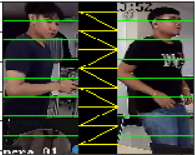
\includegraphics[width=0.3\textwidth]{chapter2/images/alignedreid.png}
		\caption{การแบ่งภาพออกเป็น 8 ส่วนของระบบระบุตัวตนของบุคคล}
    	\label{fig:alignedreid}
\end{figure}

การทำงานของระบบระบุตัวตนของบุคคลจะเริ่มจากการแบ่งภาพออกเป็น 8 ส่วนและนำคุณลักษณะทั่วไปของภาพมาผ่านกระบวนการ normalization เพื่อลดความซ้ำซ้อนของข้อมูล 
แล้วนำมาเปรียบเทียบความแตกต่างของคุณลักษณะทั่วไปของภาพโดยใช้วิธี euclidean distance หลังจากนั้นใช้วิธี DMLI หาความแตกต่างออกมา โดยค่าที่ได้ออกมาจะเรียกว่า aligned distance ถ้าค่าที่ออกมาใกล้เคียงกับศูนย์
จะหมายถึงบุคคลในภาพทั้งสองเป็นบุคคลเดียวกัน โดยใช้การกำหนดเกณฑ์ของ aligned distance สำหรับระบุตัวตนของบุคคลในภาพว่าเป็นบุคคลเดียวกันหรือไม่

โดยชุดข้อมูลที่นำมาใช้สำหรับการทำโมเดลปัญญาประดิษฐ์ได้แก่
\begin{enumerate}
	\item{Market1501 เป็นชุดข้อมูลที่เก็บข้อมูลภาพของบุคคลโดยใช้กล้องจำนวนหกตัว ถ่ายภาพบุคคลที่ด้านหน้าของซุปเปอร์มาร์เก็ตในมหาวิทยาลัย Tsinghua}
	\item{DukeMTMCReID เป็นชุดข้อมูลที่เก็บข้อมูลภาพของบุคคลโดยใช้กล้องจำนวนแปดตัว ถ่ายภาพบุคคลที่วิทยาเขตของมหาวิทยาลัย Duke ซึ่งมีการเก็บภาพมากถึงสองล้านภาพของนักศึกษาสองพันคน }
	\item{CUHK-03 เป็นชุดข้อมูลที่เก็บภาพของบุคคลที่มหาวิทยาลัยที่ฮ่องกง}
	\item{MSMT17 เป็นชุดข้อมูลที่เก็บข้อมูลภาพของบุคคลโดยใช้กล้องจำนวนสิบห้าตัว โดยที่กล้องแต่ละตัวจะไม่ได้ตั้งอยู่สถานที่เดียวกัน และเก็บข้อมูลที่ในวันที่มีสภาพอากาศต่างกัน}
\end{enumerate}

โดยทุกชุดข้อมูลจะใช้โครงสร้าง (architecture) ResNet50 ในการสร้างโมเดลปัญญาประดิษฐ์ และทดสอบด้วยวิธี Global+DMLI คือการนำคุณลักษณะทั่วไปและคุณลักษณะจำเพาะของภาพที่ได้มาจากโมเดลปัญญาประดิษฐ์ นำมาหาค่าระยะความแตกต่าง โดยที่ค่าระยะความแตกต่างของคุณลักษณะทั่วไปสามาหาได้โดยใช้วิธี Euclidean distance และค่าระยะความแตกต่างของคุณลักษณะจำเพาะสามารถหาได้โดยใช้วิธี DMLI และนำมาเทียบกับชุดข้อมูลทดสอบเพื่อคำนวณหาค่า rank1 และ mAP โดยที่ค่า rank1 หมายถึงค่าอัตราร้อยละของความมั่นใจสูงสุดของโมเดลปัญญาประดิษฐ์ที่ทำนายออกมาถูกต้อง 
และค่า mAP คือการหาค่าเฉลี่ยความแม่นยำในแต่ละหมวดหมู่ ซึ่งสามารถดูค่า rank1 และ mAP ของโมเดลปัญญาประดิษฐ์สำหรับการทำระบุตัวตนของบุคคลได้ในหัวข้อที่ \ref{sec:reid_ex}

วิธีการคำนวณของ DMLI ในขั้นตอนการสร้างโมเดลปัญญาประดิษฐ์ของการระบุตัวตนบุคคล
\begin{equation}
d_{i,j} = \frac{e^{\left \| f_{i} - g_{j} \right \|^{2}} - 1}{e^{\left \| f_{i} - g_{j} \right \|^{2}} + 1} \qquad i,j \epsilon 1,2,3,..H
\end{equation}

โดยที่
\begin{conditions}
d		&		เมทริกซ์ของระยะความแตกต่างที่น้อยที่สุดของคุณลักษณะจำเพาะของทั้งสองภาพ			\\
f		&		ค่าคุณลักษณะจำเพาะของรูปภาพที่ 1				\\
g		&		ค่าคุณลักษณะจำเพาะของรูปภาพที่ 2				\\
H		&		จำนวนภาพแนวตั่งที่แบ่งออกมา
\end{conditions}

\begin{equation}
S_{i,j} = \begin{cases}
d_{i,j} & \text{ if } i=1,j=1 \\ 
S_{i-1,j}+d_{i,j} & \text{ if } i\neq 1,j=1 \\ 
S_{i,j-1}+d_{i,j} & \text{ if } i=1,j\neq1 \\ 
min(S_{i-1,j},S_{i,j-1}) & \text{ if } i\neq1,j\neq1 
\end{cases}
\end{equation}

เมื่อทำการคำนวณ $S_{i,j}$ ซึ่งเป็นผลรวมของระยะความแตกต่างที่น้อยที่สุดแล้วตัวสุดท้ายของ $S_{i,j}$ จะเป็นระยะความแตกต่างที่น้อยที่สุดที่ของคุณลักษณะจำเพาะของทั้งสองภาพ แต่ในกรณีที่ทางผู้วิจัยนำมาใช้งานค่า $d_{i,j}$ นั้นจะเป็นค่าที่ได้มาจากการทำ euclidean distance แทน


\subsubsection*{2.1.4 การจดจำการกระทำ}
การจดจำการกระทำ เป็นกระบวนการในการทำนายการกระทำของมนุษย์หรือสิ่งที่สนใจอื่นๆ ที่เกิดการกระทำขึ้นภายในวิดีโอ โดยในหัวข้อนี้จะกล่าวถึงตั้งแต่ขั้นตอนแรกของการทำการจดจำการกระทำซึ่งก็คือ การได้มาซึ่งชุดข้อมูลมีกระบวนการอย่างไร นอกจากนั้นจะกล่าวถึงการนำ Machine learning model มาใช้ในการจดจำการกระทำ และ การวัดผลของ Machine learning model โดยชุดข้อมูลที่ผู้วิจัยได้เลือกนำมาศึกษาจากชุดข้อมูลที่ถูกเป็นที่กล่าวถึงในปัจจุบัน และ มีขนาดของชุดข้อมูลที่ใหญ่ 
\par
จากบทความข้างต้นชุดข้อมูลที่เราได้เลือกนำมาใช้ได้แก่ ชุดข้อมูล Youtube-8M , AVA , Moment in Time โดยแต่ละชุดข้อมูลจะมีความแตกต่างกันในหลายๆด้าน แต่จะมีสิ่งที่แต่ละชุดข้อมูลมีเหมือนกัน คือ เป็นชุดข้อมูลสำหรับการวิเคราะห์ผลวิดีโอที่มีการสนใจการกระทำของมนุษย์ โดยในบทความนี้จะกล่าวถึงความแตกต่างในด้านต่างๆ เช่น เป้าหมายของแต่ละชุดข้อมูล , วิธีการเก็บข้อมูลสำหรับชุดข้อมูล , วิธีการสร้างงคำอธิบาย และ รายละเอียดของชุดข้อมูล โดยจะสรุปข้อมูลของแต่ละชุดข้อมูลด้านล่าง
\begin{enumerate}
%%%%%%%%%%%%%%%%%%%%%%%%%%%%%%%%%%%%%%%%%%%%%%%%%%%%%%%%%%%%%%%%%%%%%%%%%%%%%
	\item \textbf{Youtube-8M}
	\begin{enumerate}
		\setlength\itemsep{-0.25em}
		\item เป้าหมายของชุดข้อมูล :ใช้ทำนายธีมของวิดีโอ
		\item กฏในการรวบรวมข้อมูลดังนี้
		\begin{enumerate}
			\setlength\itemsep{-0.25em}
			\item ทุกๆ หัวข้อต้องเป็นรูปธรรม
			\item ในแต่ละหัวข้อต้องมีจำนวนวิดีโอไม่น้อยกว่า 200 วิดีโอ
			\item ความยาวของวิดีโอต้องอยู่ระหว่าง 120 - 500 วินาที
		\end{enumerate}
		หลังจากได้กฏในการรวบรวมข้อมูลแล้ว ขั้นตอนต่อไปคือการสร้างคำศัพท์ที่ใช้ในการค้นหาข้อมูลวิดีโอจากใน YouTube 
		\item ขั้นตอนในการสร้างคำศัพท์มีดังนี้
		\begin{enumerate}
			\setlength\itemsep{-0.25em}
			\item กำหนด whitelist หัวข้อที่เป็นรูปธรรมมา 25 ชนิด เช่น เกมส์ เป็นต้น
			\item กำหนด blacklist หัวข้อที่คิดว่าไม่เป็นรูปธรรมไว้ เช่น software เป็นต้น
			\item รวบรวมหัวข้อที่มีอยู่ใน whitelist อย่างน้อย 1 หัวข้อ และต้องไม่มีอยู่ใน blacklist ซึ่งจะทำให้ได้หัวข้อที่ต้องการมาประมาณ 50,000 หัวข้อ
			\item จากนั้นใช้ผู้ประเมินจำนวน 3 คน ในการคัดหัวข้อที่คิดว่าเป็นรูปธรรม และสามารถจดจำหรือเข้าใจได้ง่ายโดยไม่ต้องเชี่ยวชาญในด้านนั้นๆ ซึ่งผู้ประเมิน ก็จะมีคำถามว่า “ มันยากขนาดไหนถึงจะระบุได้ว่ามีหัวข้อดังกล่าวอยู่ในรูปหรือวิดีโอ โดยใช้เพียงแค่การมองรูปภาพเท่านั้น? ” โดยแบ่งเป็นระดับดังนี้
			\begin{enumerate}
				\setlength\itemsep{-0.25em}
				\item บุคคลทั่วไปสามารถเข้าใจได้
				\item บุคคลทั่วไปที่ผ่านการอ่านบทความที่เกี่ยวข้องมาแล้วสามารถเข้าใจได้
				\item ต้องเชี่ยญในด้านใดซักด้านจึงจะเข้าใจได้
				\item เป็นไปไม่ได้ ถ้าไม่มีความรู้ที่ไม่ได้เป็นรูปธรรม
				\item ไม่เป็นรูปธรรม
			\end{enumerate}
			\item หลังจากคำถามข้างบนและการให้คะแนน จะทำการเก็บไว้เฉพาะหัวข้อที่มีคะแนนเฉลี่ยมากที่สุดอยู่ที่ประมาณ 2.5 คะแนนเท่านั้น
			\item ทำให้สุดท้ายเหลือเพียงประมาณ 10,000 หัวข้อที่สามารถใช้ได้
			\item หลังจากได้หัวข้อที่คิดว่าเป็นรูปธรรมแล้วก็นำไปค้นหาและรวบรวมด้วย YouTube annotation system โดยมีขั้นตอนดังนี้										\begin{enumerate}
				\setlength\itemsep{-0.25em}
				\item สุ่มเลือกวิดีโอมา 10 ล้านวิดีโอ พร้อมกับหัวข้อของวิดีโอ โดยใช้กฏที่กำหนดไว้ เอาหัวข้อที่มีจำนวนวิดีโอน้อยกว่า 200 วิดีโอออก
				\item ทำให้เหลือจำนวนวิดีโออยู่ 8,264,650 วิดีโอ
				\item แยกออกเป็น 3 ส่วน Train set, Validate set และ Test set ในอัตราส่วน 70:20:10 ตามลำดับ
			\end{enumerate}
		\end{enumerate}
	\end{enumerate}
%%%%%%%%%%%%%%%%%%%%%%%%%%%%%%%%%%%%%%%%%%%%%%%%%%%%%%%%%%%%%%%%%%%%%%%%%%%%%
	\item \textbf{AVA}
	\begin{enumerate}
		\setlength\itemsep{-0.25em}
		\item เป้าหมายของชุดข้อมูล : สนใจการกระทำของมนุษย์เป็นศูนย์กลาง
		\item ขั้นตอนการเก็บข้อมูลสำหรับการทำชุดข้อมูลมีขั้นตอนการทำ 5 ขั้น คือ
	\begin{enumerate}
%
		\item การสร้างคำศัพท์การกระทำ จะมีหลัก 3 ข้อในการรวบรวมคำศัพท์ คือ
		\begin{enumerate}
			\item เก็บรวบรวมคำศัพท์ทั่วไปที่เกิดขึ้นในชีวิตประจำวัน
			\item จะต้องมีเอกลักษณ์ สามาถเห็นได้ชัดเจน เช่น การถือของ
			\item กำหนดรูปแบบของคำศัพท์ขึ้นมาและใช้ความรู้จากชุดข้อมูลอื่น ในการทำให้ได้หมวดหมู่ของการกระทำของมนุษย์ที่ครอบคลุมของชุดข้อมูล AVA
		\end{enumerate}
		\setlength\itemsep{-0.25em}
%
		\item  หนังและส่วนที่เลือกมาใช้วิดิโอที่ใช้ทำชุดข้อมูล AVA ทั้งหมดจะถูกนำมากจาก youtube โดยเริ่มจากการรวบรวมเอารายชื่อของนักแสดงที่มีชื่อเสียง ซึ่งจะมีความหลากหลายของเชื้อชาติรวมกันอยู่ ซึ่งวิดิโอที่ถูกคัดเลือกจะมีเกณฑ์ดังนี้ คือ
			\begin{enumerate}
				\item วิดิโอต้องอยู่ในหมวด หนัง และ ละครโทรทัศน์
				\item จะต้องมีความยาวมากกว่า 30 นาที
				\item อัพโหลดเป็นเวลาอย่างน้อย 1 ปี
				\item มียอดวิวคนดูมากกว่า 1000 วิว
				\item ละเว้นวิดิโอบางประเภท เช่น ขาว-ดำ , ความละเอียดต่ำ , การ์ตูน , วิดิโอเกม
			\end{enumerate}
%
		\item  การตีกรอบบุคคลที่อยู่ภายในภาพ ประกอบด้วย 2 ขั้นตอน
			\begin{enumerate}
				\item สร้างกรอบสี่เหลี่ยม โดยใช้โมเดล Faster R-CNN สำหรับการตรวจจับมนุษย์
				\item นำมนุษย์มาใช้ในการตรวจสอบและแก้ไขกรอบสี่เหลี่ยมที่พลาดไป หรือ ตรวจจับผิด
			\end{enumerate}	
		\item  การเชื่อมของบุคคลในช่วงระยะเวลาสั้นๆของเฟรม 
\\
ทำการเชื่อมกรอบสี่เหลี่ยมที่อยู่ในช่วงเวลาเดียวกัน ซึ่งใช้วิธีการ track โดยยึดมนุษย์เป็นศูนย์กลาง ซึ่งจะนำมาคำนวณความใกล้เคียงกันโดยการจับคู่กรอบสี่เหลี่ยม และ ใช้ person embedding จากนั้นจะใช้ Hungarian algorithm ในการหาตัวเลือกที่ดีที่สุด

%
		\item การสร้างคำอธิบาย
\\
		การสร้างคำอธิบายของการกระทำจะถูกสร้างจากเหล่าคนที่เป็นผู้สร้างคำอธิบาย ซึ่งจะใช้หน้าต่างโปรแกรมสำหรับช่วยเหลือในการสร้างซึ่งใน 1 กรอบสี่เหลี่ยม สามารถมีคำอธิบายของการกระทำได้สูงสุดถึง 7 labels นอกจากนั้นสามารถตั้งสถานะบล็อกเนื้อหาที่ไม่เหมาะสม หรือ กรอบสี่เหลี่ยมที่ผิดพลาดได้อีกด้วย ในทางปฎิบัติจะสังเกตได้ว่ามันมีโอกาศผิดอย่างหลีกเลี่ยงไม่ได้ เมื่อต้องได้รับคำสั่งให้หาคำอธิบายของการกระทำที่ถูกต้องจาก 80 หมวดหมู่ จึงแบ่งขั้นตอนออกเป็น 2 ขั้นตอน คือ
		\begin{enumerate}
			\item ข้อเสนอของการกระทำสอบถามเหล่าผู้สร้างคำอธิบาย เพื่อสร้างข้อเสนอสำหรับคำอธิบายของการกระทำจากนั้นจับกลุ่มเข้าด้วยกัน ซึ่งจะทำให้มีโอกาสถูกต้องมากกว่าเป็นข้อเสนอแยกเดี่ยว
			\setlength\itemsep{-0.25em}
			\item ผู้ตรวจสอบข้อเสนอจะตรวจสอบข้อเสนอที่ได้จากขั้นตอนแรก ซึ่งในแต่ละวิดิโอคลิปจะใช้มนุษย์ในการตรวจสอบ 3 คน เมื่อคำอธิบายของการกระทำ ถูกตรวจสอบด้วยผู้ตรวจสอบข้อเสนออย่างน้อย 2 คน คำอธิบายของการกระทำนั้นจะถูกยึดเป็นคำอธิบายหลัก
		\end{enumerate}
	\end{enumerate}
	\end{enumerate}
%%%%%%%%%%%%%%%%%%%%%%%%%%%%%%%%%%%%%%%%%%%%%%%%%%%%%%%%%%%%%%%%%%%%%%%%%%%%
	\item \textbf{Moment in Time}
	\begin{enumerate}
		\setlength\itemsep{-0.25em}
		\item เป้าหมายของชุดข้อมูล : สนใจการกระทำทุกการกระทำในวิดิโอ เช่น การกระทำของ คน สัตว์ สิ่งของ และ ปรากฎการณ์ธรรมชาติ 
		\item วิธีการเก็บรวบรวมข้อมูล : 
	\begin{enumerate}
	\item เริ่มจากการรวบรวมคำ (verb) ที่มีการใช้อยู่ทั่วไปในชีวิตประจำวันมา 4,500 คำจาก VerbNet จากนั้นนำมาแบ่งกลุ่มคำ(verb) ที่มีความหมายใกล้เคียงกันโดยใช้ features จาก Propbank และ FrameNet โดยเก็บข้อมูลเป็นแบบ binary feature vector ซึ่งถ้าคำ (verb) ไหนมีความเกี่ยวข้องกับ feature ก็จะให้ค่าเป็น 1 ถ้าไม่เกี่ยวข้องกันจะให้ค่าเป็น 0 จากนั้นจึงใช้วิธี k-means clustering ในการแบ่งกลุ่ม เมื่อแบ่งกลุ่มแล้วจากนั้นจะเลือกคำ (verb) จากในแต่ละกลุ่มนั้น โดยคำ (verb) ที่เลือกมานั้นจะเป็นที่ใช้บ่อยที่สุดในกลุ่มนั้น และลบคำ (verb) นั้นออกจากกลุ่มทั้งหมด (คำ ๆ หนึ่งสามารถอยู่ได้หลายกลุ่ม) จากนั้นจะทำกระบวนการนี่ไปเรื่อย ๆ แต่คำ (verb) ที่เลือกมาจะต้องไม่มีความหมายคลุมเครือ ไม่สามารถมองเห็นหรือได้ยินได้ และต้องไม่มีความหมายเหมือนกับคำ (verb) ที่เคยเลือกมาก่อน จนสุดท้ายแล้วได้ออกมาที่ 339 class
	\item ต่อมาทำการหาชุดข้อมูลวิดีโอโดยจะตัดออกมาเพียง 3 วินาทีที่เกี่ยวข้องกับคำ (verb) ใน 339 class ที่เลือกมา จากวิดีโอ แหล่งต่างกัน 10 แหล่ง การตัดวิดีโอนั้นจะไม่ใช้พวก Video2Gif (โมเดลที่ระบุตำแหน่งของสิ่งที่น่าสนใจในวิดีโอ) เพราะจะทำให้เกิด bias ขึ้นจะเกิดขึ้นตอนสร้างโมเดลจากนั้นจะทำการส่งข้อมูลของคำ (verb) และวิดีโอที่ตัดไปยัง Amazon Mechanical Turk (AMT หรือตลาดแรงงาน) เพื่อทำการ label โดยพนักงานแต่ละคนของ AMT จะได้ 64 วิดีโอซึ่งเกี่ยวข้องกับคำ (verb) หนึ่ง และอีก 10 วิดีโอที่มีการทำ label อยู่แล้ว โดยวิดีโอที่มีการทำ label ถ้ามีพนักงานของ AMT ตอบเหมือนกันกับที่ทำ label ไว้เกิน 90\% ถึงจะนำเข้าไปรวมกับชุดข้อมูลส่วนอีก 64 วิดีโอถ้าเป็นของ training set จะต้องผ่านพนักงานของ AMT อย่างน้อย 3 ครั้ง และต้อง label เหมือนกัน 75\% ขึ้นไปถึงจะถือว่าเป็น label ที่ถูกต้อง ถ้าเป็นของ validation และ test set จะต้องผ่านพนักงานของ AMT อย่างน้อย 4 ครั้ง และต้อง label เหมือนกัน 85\% ขึ้นไป ที่ไม่ตั่งเกณฑ์ไว้ที่ 100\% เพราะจะทำให้วิดีโอนั้นยากเกินไปที่จะทำให้สามารถจำการกระทำได้	
\end{enumerate}
\end{enumerate}
%%%%%%%%%%%%%%%%%%%%%%%%%%%%%%%%%%%%%%%%%%%%%%%%%%%%%%%%%%%%%%%%%%%%%%%%%%%%
\end{enumerate}		

\clearpage
\section{เครื่องมือสำหรับการวิเคราะห์ผลวิดีโอ}
\subsection{โมเดลปัญญาประดิษฐ์สำหรับจำแนกการกระทำมนุษย์}
\subsubsection{ResNet}
ในการสร้างโมเดลปัญญาประดิษฐ์นั้นการใช้จำนวนชั้นเยอะนั้นจะทำให้ได้คุณลักษณะของข้อมูลที่ออกมาเยอะตามไปด้วย 
แต่การที่คุณลักษณะของข้อมูลเยอะไม่ได้หมายความว่าโมเดลปัญญาประดิษฐ์จะให้ประสิทธิภาพที่ดีเสมอไป ซึ่งสามารถแก้ปัญหานี้ได้โดยใช้ residual network (ResNet)\textsuperscript{\cite{he2016deep}} 
ซึ่งเป็น CNN ประเภทหนึ่ง ที่ส่วนใหญ่จะนำมาใช้กับข้อมูลที่เป็นภาพ เช่น การจดจำวัตถุ เป็นต้น โดย ResNet นี้จะสามารถทำการข้ามชั้นที่ไม่จำเป็นได้ 
การข้ามชั้นที่ไม่จำเป็นจะช่วยให้ข้อมูลที่ได้ออกมานั้นดีที่สุด

\begin{figure}[!ht]
	\centering
	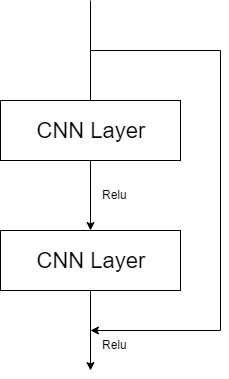
\includegraphics[width=0.2\textwidth]{chapter2/images/example_resnet.png}
		\caption{หลักการของ Residual block ของ ResNet}
    	\label{fig:ResNet}
\end{figure}

การทดลองโมเดลปัญญาประดิษฐ์ ResNet ด้วยการทำจำแนกภาพโดยใช้ชุดข้อมูลทดสอบ ImageNet ที่มีหมวดหมู่มากกว่า 1,000 หมวดหมู่
มาเทียบกับโมเดลปัญญาประดิษฐ์ทั่วไป (plain model) ที่จำนวนชั้น 18 ชั้น และ 34 ชั้น โดยโครงสร้างพื้นฐานของโมเดลปัญญาดิษฐ์ ResNet และโมเดลปัญญาประดิษฐ์ทั่วไปเหมือนกัน 
ซึ่งผลลัพธ์อัตราร้อยละของความผิดพลาดจะได้ออกมาตามตารางที่ \ref{tab: Top-1 error of ImageNet} 

\begin{table}[!ht]
	\centering
	\begin{tabular}{|c|c|c|}
		\hline
		{จำนวนชั้นของโมเดลปัญญาประดิษฐ์}&\multicolumn{2}{c|}{Training error}\\
		\cline{2-3}
		{}							& plain						& ResNet			\\
		\hline
		18							& 27.94						& 27.88				\\
		34							& 28.54						& 25.03				\\
		\hline
	\end{tabular}
	\caption{อัตราร้อยละของความผิดพลาดของชุดข้อมูลทดสอบ ImageNet}
	\label{tab: Top-1 error of ImageNet}
\end{table}

จากตาราง \ref{tab: Top-1 error of ImageNet} จะเห็นได้ว่าโมเดลปัญญาประดิษฐ์ทั่วไป 34 ชั้นมีค่าอัตราร้อยละของความผิดพลาดสูงกว่าโมเดลปัญญาประดิษฐ์ ResNet 
ได้อย่างชัดเจน ในขณะที่โมเดลปัญญาประดิษฐ์ทั่วไปจะมีอัตราร้อยละของความผิดพลาดสูงขึ้นเมื่อเทียบกันระหว่าง 18 ชั้นและ 34 ชั้น
\clearpage
ต่อมาจะนำโมเดลปัญญาประดิษฐ์ ResNet มาทดสอบกับชุดข้อมูล CIFAR-10 ซึ่งเป็นชุดข้อมูลที่มีรูปสำหรับใช้สร้างโมเดลปัญญาประดิษฐ์ 50,000 รูป รูปสำหรับทดสอบ 10,000 รูป 
และมีจำนวนหมวดหมู่ทั้งหมด 10 หมวดหมู่ โดยจะมีการออกแบบของจำนวนชั้นของโมเดลปัญญาประดิษฐ์ ResNet ตามจำนวนของชั้น convolution 
ที่มีผังคุณลักษณะเท่ากัน 6 ชั้นติดกันและการข้ามชั้นทีละ 2 ชั้น จึงทำให้ได้รูปแบบการคิดชั้นดังนี้ 6n + 2 สำหรับการทดสอบจะให้ค่า n = [3, 5, 7, 9, 200] ดังตารางต่อไปนี้

\begin{table}[!ht]
	\centering
	\begin{tabular}{|c|c|c|}
		\hline
		{โมเดลปัญญาประดิษฐ์}		  &{จำนวนชั้น}				    &{Training error}	\\
		\hline
		ResNet						& 20						& 8.75				\\
		ResNet						& 32						& 7.51				\\
		ResNet						& 44						& 7.17				\\
		ResNet						& 56						& 6.97				\\
		ResNet						& 110						& 6.43				\\
		ResNet						& 1202						& 7.93				\\
		\hline
	\end{tabular}
	\caption{ค่าความผิดพลาดที่ได้จากการทดลองจำนวนชั้นของโมเดลปัญญาประดิษฐ์ ResNet บนชุดของข้อมูล CIFAR-10}
	\label{tab: หมวดหมู่ification error}
\end{table}
จากตาราง \ref{tab: หมวดหมู่ification error} จะเห็นได้ว่าที่โมเดลปัญญาประดิษฐ์ ResNet ที่มีจำนวนชั้น 1,202 
นั้นมีค่าความผิดพลาดเกิดขึ้นมากกว่าจำนวนชั้น 110 ซึ่งอาจจะเป็นไปได้ว่าขนาดของโมเดลปัญญาประดิษฐ์ ResNet ที่มีจำนวนชั้น 1,202 
นั้นมากเกินไปสำหรับชุดข้อมูลขนาดเล็กนี้
\subsubsection{Inflated 3D convolutional network}
ในการพัฒนาโมเดลปัญญาประดิษฐ์สำหรับจำแนกการกระทำของมนุษย์นั้นมีพื้นฐานมาจากการจำแนกวัตถุ (object classification)
หมายถึงการใช้รูปภาพหนึ่งรูปในการประมวลผลและทำนายออกมาว่าภายในรูปนั้นมีบริบทการกระทำอย่างไร โดยไม่ได้คำนึงถึงข้อมูลเชิงต่อเนื่อง (spatio-temporal information)
จากบทความ "Quo Vadis, Action Recognition? A New Model and the Kinetics Dataset"\textsuperscript{\cite{I3D}} นั้นได้พัฒนาโครงสร้างของโมเดลปัญญาประดิษฐ์ (architecture) 
ที่มีประสิทธิภาพในการประมวลผลภาพเคลื่อนไหวได้ชื่อว่า I3D หรือ inflated 3D convolution network
โดยโครงสร้างพื้นฐานของ I3D นั้นมาจาก Inception-v1\textsuperscript{\cite{Inception}} ที่ถูกพัฒนาโดย Goggle ซึ่งเป็นโครงสร้างที่มีประสิทธิภาพสูงในการจำแนกวัตถุในรูปภาพ
แล้ว I3D นั้นได้ทำการขยายมิติของโครงสร้างจาก 2 มิติ เป็น 3 มิติ เพื่อให้โมเดลปัญญาประดิษฐ์สามารถเรียนรู้ข้อมูลเชิงต่อเนื่องได้
\begin{figure}[!ht]
    \centering
    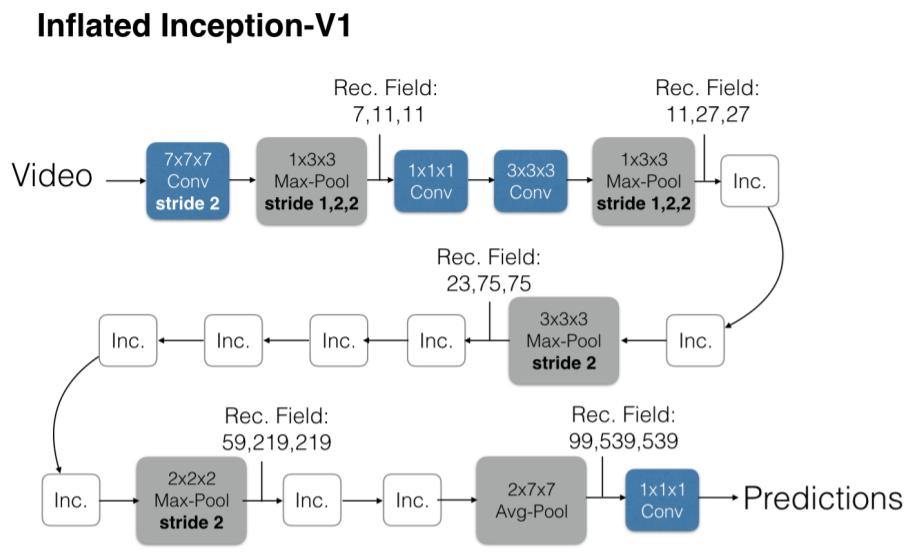
\includegraphics[width=1.0\textwidth]{chapter2/images/I3D.png}
    \caption{โครงสร้างของโมเดลปัญญาประดิษฐ์ I3D\textsuperscript{\cite{I3D}}}
    \label{fig:I3DArch}
\end{figure}

\begin{figure}[!ht]
    \centering
    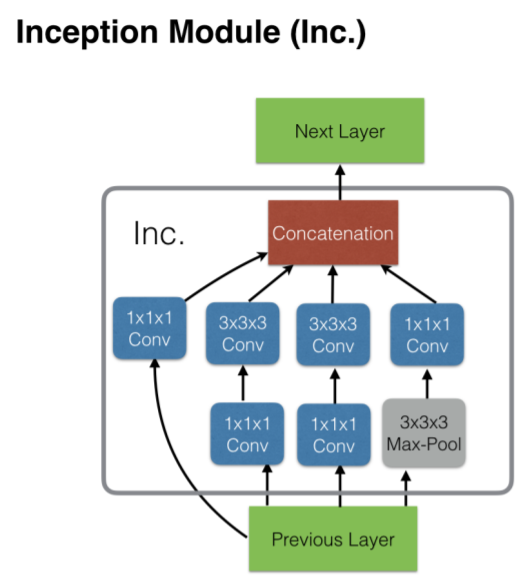
\includegraphics[width=0.7\textwidth]{chapter2/images/inceptionModule.png}
    \caption{โครงสร้างของโมเดลปัญญาประดิษฐ์ I3D\textsuperscript{\cite{I3D}}}
    \label{fig:I3DArch}
\end{figure}
% ตารางที่ \ref{tab:I3DPerformance}

\clearpage

\subsection{เครื่องมือสำหรับสร้างชุดข้อมูล}
จากการค้นคว้าหาเครื่องมือในการสร้างคำกำกับข้อมูลเพื่อใช้เป็นแนวทางในการออกเครื่องมือสำหรับกำกับข้อมูลด้วยปัญญาประดิษฐ์ พบเครื่องมือที่เปิดให้ใช้ง่นสาธารณะ (open source) 2 เครื่องมือ 
คือ DarkLabel และ OpenLabeling โดยสรุปข้อสำคัญได้ดังนี้ 
\subsubsection*{โปรแกรม DarkLabel}
เป็นโปรแกรมที่ช่วยในการทำนายคำกำกับและบันทึกในรูปแบบต่างๆ รองรับข้อมูลป้อนเข้าในรูปแบบไฟล์วิดีโอ avi, mpg หรือกลุ่มรูปภาพ มีขั้นตอนการสร้างคำกำกับดังนี้ 
\begin{enumerate}
	\setlength\itemsep{-0.25em}
	\item สร้างกรอบสี่เหลี่ยมครอบบริเวณวัตถุที่สนใจโดยใช้มนุษย์เป็นคนสร้าง
	\item กดปุ่ม Next และ Predict อย่างต่อเนื่อง เพื่อทำนายตำแหน่งต่อไปของกรอบสี่เหลี่ยมในเฟรมถัดๆไป จนกระทั่งการเกิดข้อผิดพลาด
	\item ลบกรอบสี่เหลี่ยมที่พลาด และเริ่มทำขั้นตอนที่ 1 ใหม่ อีกครั้งจนครบทุกเฟรมในวิดีโอ
\end{enumerate}
หลังจากที่ผู้วิจัยได้ทดลองใช้โปรแกรม DarkLabel พบว่า เป็นโปรแกรมที่การทำงานส่วนใหญ่เป็นการสร้างคำกำกับแบบใช้มนุษย์เป็นคนทำด้วยตัวเอง ซึ่งทำให้ใช้เวลาในการทำนาน

\begin{figure}[!ht]
	\centering
	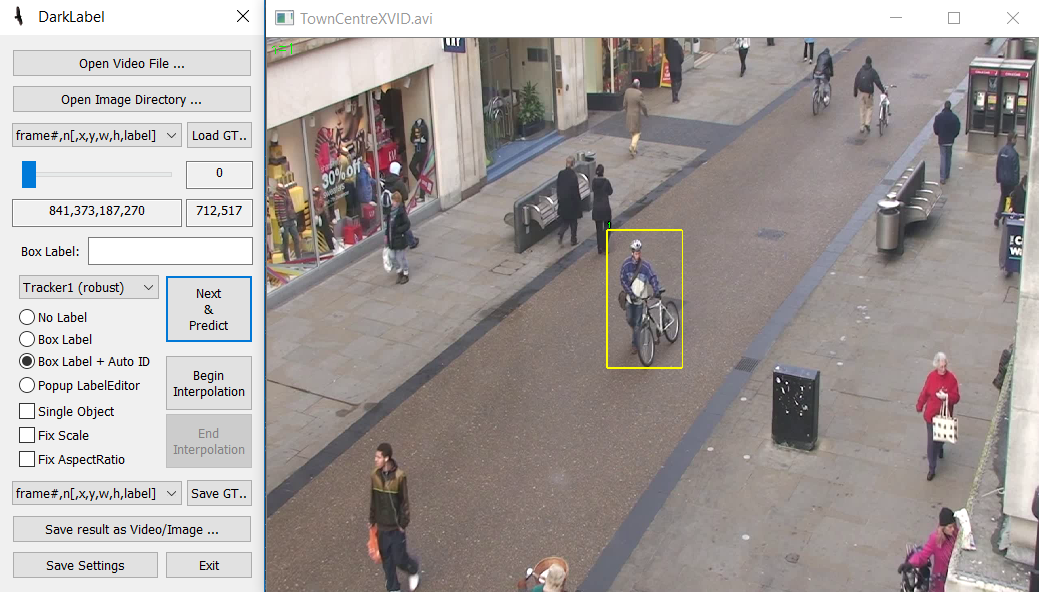
\includegraphics[width=0.7\textwidth]{chapter2/images/darklabel.png}
		\caption{UI ของโปรแกรม DarkLabel}
    	\label{fig:darklabel}
\end{figure}
\clearpage

\subsubsection*{โปรแกรม OpenLabeling}
เป็นโปรแกรมที่ช่วยในการทำนายคำกำกับ โดยโปรแกรมจะมีการทำงานอยู่ 2 รูปแบบการทำงาน คือแบบทำด้วยตัวเอง (Mode Manual) และแบบอัตโนมัติ (Mode Auto) ซึ่งมีการทำงานแยกจากกันอย่างชัดเจน 

\begin{enumerate}
	\setlength\itemsep{-0.25em}
	\item การทำงานแบบอัตโนมัติ 
	\\ หลังจากป้อนวิดีโอเข้าไปในโปรแกรมแล้วมีขั้นตอนการสร้างคำกำกับดังนี้ 
   	\begin{enumerate}
	\setlength\itemsep{-0.25em}
		\item โปรแกรมจะทำงานอัตโนมัติ โดยใช้โมเดลปัญญาประดิษฐ์ในการทำนายคีย์เฟรม (keyframe) 
		และทำนายตำแหน่งต่อไปของกรอบสี่เหลี่ยมในเฟรมถัดไปด้วยอัลกอริทึมที่ใช้การคำนวณคณิตศาสตร์และการประมวลผลภาพ (image processing) ในภาพที่เหลือ ผลลัพธ์ที่ได้คือรูปภาพและไฟล์ข้อมูลคำกำกับ
 	\end{enumerate}
	\item การทำงานแบบทำด้วยตัวเอง 
	\\ หลังจากป้อนวิดีโอเข้าไปในโปรแกรมแล้วมีขั้นตอนการสร้างคำกำกับดังนี้ 
	\begin{enumerate}
	\setlength\itemsep{-0.25em}
		\item สร้างกรอบสี่เหลี่ยมขึ้นมาโดยใช้มนุษย์เป็นคนสร้าง
		\item กดปุ่มเพื่อทำนายตำแหน่งต่อไปของกรอบสี่เหลี่ยมในเฟรมถัดไป จนกระทั่งเกิดข้อผิดพลาด
		\item ลบกรอบสี่เหลี่ยมที่พลาด และเริ่มทำขั้นตอนที่ 1 อีกครั้งจนครบทุกเฟรมในวิดีโอ
 	\end{enumerate}
 \end{enumerate}
หลังจากที่ได้ทดลองใช้โปรแกรม OpenLabeling ทั้ง 2 รูปแบบการทำงานแล้วพบว่า การทำงานแบบอัตโนมัติไม่สามารถปรับแก้ไขสิ่งใดในระหว่างกระบวนการนั้น 
ทำให้หากเกิดกรณีที่โมเดลทำนายกรอบสี่เหลี่ยมพลาดหรือเกินมา จะไม่สามารถแก้ไขได้ และการทำงานแบบทำด้วยตัวเองไม่มีระบบตรวจสอบกรอบสี่เหลี่ยม ทำให้ผู้ใช้งานจะต้องสร้างกรอบสี่เหลี่ยมขึ้นมาเอง

\begin{figure}[!ht]
	\centering
	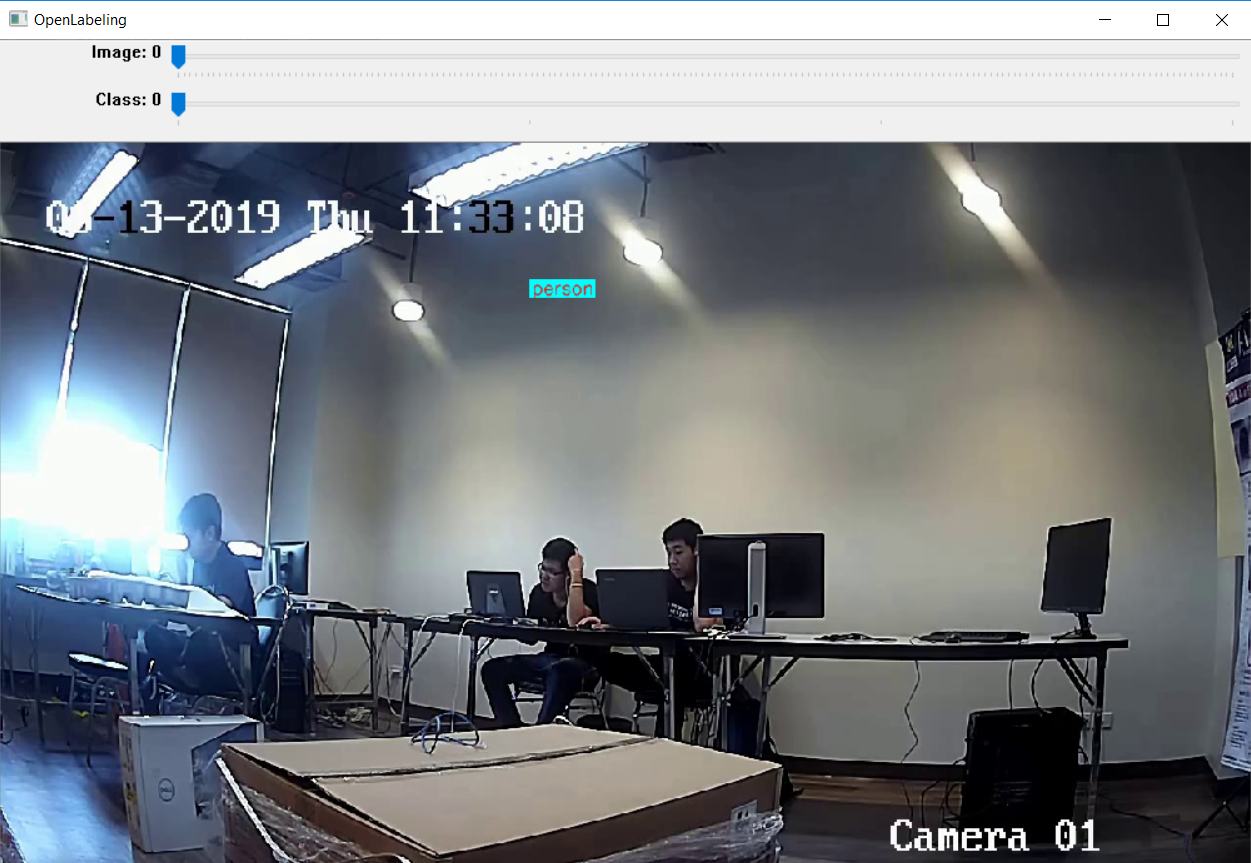
\includegraphics[width=0.7\textwidth]{chapter2/images/openlabel.png}
		\caption{UI ของโปรแกรม OpenLabeling}
    	\label{fig:openlabel}
\end{figure}




\clearpage
%\section{ชุดข้อมูล}
%\subsubsection*{Youtube-8M}
YouTube-8M คือชุดข้อมูลวิดีโอที่เป็น multi-label ที่มีจำนวนวิดีโอเยอะที่สุด ซึ่งมีจำนวนมากถึง 8 ล้านวิดีโอ(ในปี 2016) โดยมีจุดมุ่งหมายหลักในการอธิบายธีมหลักของวิดีโอด้วยคำสั้นๆ เช่น ถ้าวิดีโอนั้นเป็นวิดีโอที่มี มนุษย์กำลังปั่นจักรยานบนถนนดินกับหน้าผา ชุดข้อมูลนี้จะอธิบายวิดีโอนี้ว่า mountain biking ซึ่งทำให้ YouTube-8M แตกต่างจากชุดข้อมูลวิดีโออื่นๆส่วนใหญ่ที่จะเน้น action หรือ activity ของมนุษย์ ซึ่งข้อมูลเชิงสถิติจะเป็นดังตารางที่ 1

\begin{figure}[!ht]
	\centering
	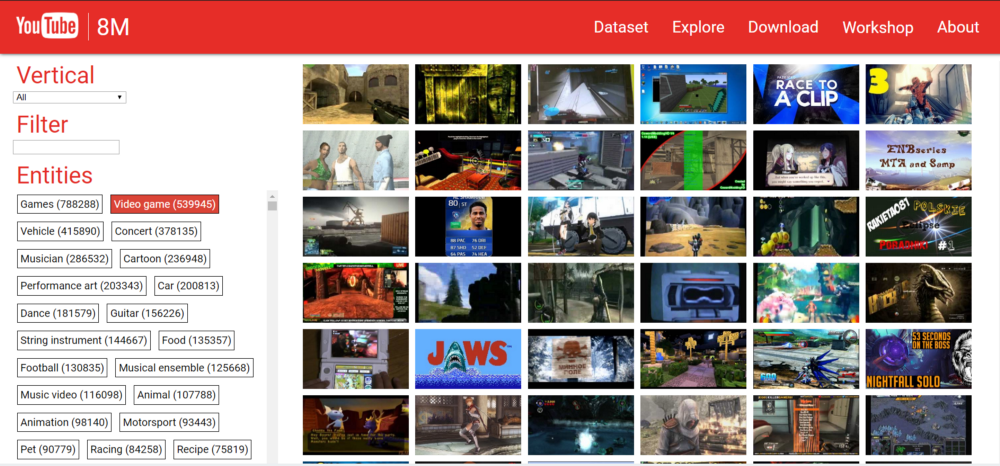
\includegraphics[width=1\textwidth]{chapter2/images/youtube-8m.png}
		\caption{ตัวอย่าง catagories ต่างๆของ YouTube-8M}
    	\label{fig:youtube-8m}
\end{figure}

\begin{table}[!ht]
\begin{tabular}{|c|c|c|c|c|}
		\hline
		{จำนวนวิดีโอ}&{ความยาวโดยรวมของวิดีโอ(ชม.)}&{จำนวนคลาสของวิดีโอ}&{ความยาวเฉลี่ยของแต่ละวิดีโอ(วินาที)}&{(จำนวนคลาสเฉลี่ยในแต่ละวิดีโอ)}\\
		\hline
		8,264,650			& ~500,000		& 4800		& 229.6		& 1.8											\\
		\hline
	\end{tabular}
	\caption{ข้อมูลเชิงสถิติของ YouTube-8M}
	\label{tab: ข้อมูลเชิงสถิติของ YouTube-8M}
\end{table}

\subsubsection*{1. วิธีการรวบรวมข้อมูล}
การเก็บข้อมูลของ YouTube-8M นั้นใช้เครื่องมือที่ชื่อว่า YouTube annotation system ในการเก็บรวบรวมข้อมูลโดยอาศัยผังความรู้(knowledge graph)ของ Google ในการค้นหาและรวบรวมข้อมูลในฐานข้อมูลของ YouTube
\begin{enumerate}
	\setlength\itemsep{-0.25em}
	\item กฏในการรวบรวมข้อมูลดังนี้
	\begin{enumerate}
		\setlength\itemsep{-0.25em}
		\item ทุกๆ หัวข้อต้องเป็นรูปธรรม
		\item ในแต่ละหัวข้อต้องมีจำนวนวิดีโอไม่น้อยกว่า 200 วิดีโอ
		\item ความยาวของวิดีโอต้องอยู่ระหว่าง 120 - 500 วินาที
	\end{enumerate}
หลังจากได้กฏในการรวบรวมข้อมูลแล้ว ขั้นตอนต่อไปคือการสร้างคำศัพท์(vocabulary)ที่ใช้ในการค้นหาข้อมูลวิดีโอจากใน YouTube 
	\item ขั้นตอนในการสร้างคำศัพท์มีดังนี้
	\begin{enumerate}
		\setlength\itemsep{-0.25em}
		\item กำหนด whitelist หัวข้อที่เป็นรูปธรรมมา 25 ชนิด เช่น game เป็นต้น
		\item กำหนด blacklist หัวข้อที่คิดว่าไม่เป็นรูปธรรมไว้ เช่น software เป็นต้น
		\item รวบรวมหัวข้อที่มีอยู่ใน whitelist อย่างน้อย 1 หัวข้อ และต้องไม่มีอยู่ใน blacklist ซึ่งจะทำให้ได้หัวข้อที่ต้องการมาประมาณ 50,000 หัวข้อ
		\item จากนั้นใช้ผู้ประเมินจำนวน 3 คน ในการคัดหัวข้อที่คิดว่าเป็นรูปธรรม และสามารถจดจำหรือเข้าใจได้ง่ายโดยไม่ต้องเชี่ยวชาญในด้านนั้นๆ ซึ่งผู้ประเมิน ก็จะมีคำถามว่า “ มันยากขนาดไหนถึงจะระบุได้ว่ามีหัวข้อดังกล่าวอยู่ในรูปหรือวิดีโอ โดยใช้เพียงแค่การมองรูปภาพเท่านั้น? ” โดยแบ่งเป็นระดับดังนี้
		\begin{enumerate}
			\setlength\itemsep{-0.25em}
			\item บุคคลทั่วไปสามารถเข้าใจได้
			\item บุคคลทั่วไปที่ผ่านการอ่านบทความที่เกี่ยวข้องมาแล้วสามารถเข้าใจได้
			\item ต้องเชี่ยญในด้านใดซักด้านจึงจะเข้าใจได้
			\item เป็นไปไม่ได้ ถ้าไม่มีความรู้ที่ไม่ได้เป็นรูปธรรม
			\item ไม่เป็นรูปธรรม
		\end{enumerate}
		\item หลังจากคำถามข้างบนและการให้คะแนน จะทำการเก็บไว้เฉพาะหัวข้อที่มีคะแนนเฉลี่ยมากที่สุดอยู่ที่ประมาณ 2.5 คะแนนเท่านั้น
		\item ทำให้สุดท้ายเหลือเพียงประมาณ 10,000 หัวข้อที่สามารถใช้ได้
		\item หลังจากได้หัวข้อที่คิดว่าเป็นรูปธรรมแล้วก็นำไปค้นหาและรวบรวมด้วย YouTube annotation system โดยมีขั้นตอนดังนี้
		\begin{enumerate}
			\setlength\itemsep{-0.25em}
			\item สุ่มเลือกวิดีโอมา 10 ล้านวิดีโอ พร้อมกับหัวข้อของวิดีโอ โดยใช้กฏที่กำหนดไว้ เอาหัวข้อที่มีจำนวนวิดีโอน้อยกว่า 200 วิดีโอออก
			\item ทำให้เหลือจำนวนวิดีโออยู่ 8,264,650 วิดีโอ
			\item แยกออกเป็น 3 ส่วน Train set, Validate set และ Test set ในอัตราส่วน 70:20:10 ตามลำดับ
		\end{enumerate}
	\end{enumerate}
\end{enumerate}

เนื่องจากชุดข้อมูลนี้มีขนาดมากกว่า 100 Terabytes และมีความยาวรวมประมาณ 500,000 ชั่วโมง ทำให้การจะใช้คอมพิวเตอร์ทั่วไปเปิดอาจจะใช้เวลานานถึง 50 ปี ทำให้ Google ทำการลดขนาดของข้อมูลลงโดยมีขั้นตอนดังนี้
\begin{figure}[!ht]
	\centering
	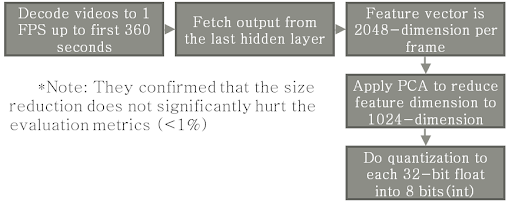
\includegraphics[width=1\textwidth]{chapter2/images/decrease_data.png}
		\caption{ขั้นตอนกระบวนการการลดขนาดของชุดข้อมูลให้สามารถใช้งานได้ง่ายยิ่งขึ้น}
    	\label{fig:decrease_data}
\end{figure}




\subsubsection*{2. การทดลองและวิเคราะห์ผล}
ในบทความ \footnote{YouTube-8M,https://arxiv.org/pdf/1609.08675.pdf} นั้นได้นำเสนอวิธีการในการจัดการข้อมูลซึ่งแบ่งเป็น 2 รูปแบบตามลักษณะของข้อมูลที่ใช้ และอัลกอริทึมหรือเทคนิคที่ใช้ในการสร้างโมเดล ดังนี้
\begin{enumerate}
	\setlength\itemsep{-0.25em}
	\item คุณลักษณะระดับเฟรม (Frame-level feature)
	\begin{enumerate}
		\setlength\itemsep{-0.25em}
		\item Frame-Level Models and Average Pooling
		\\ อันดับแรกเนื่องจากว่าชุดข้อมูลนี้ไม่มีการระบุหัวข้อในระดับเฟรม จึงใช้วิธีการนำหัวข้อในระดับวิดีโอ มากำหนดให้กับทุกๆเฟรมในวิดีโอแทน จากนั้นสุ่มเฟรมมา 20 เฟรมในแต่ละวิดีโอ ทำให้มีเฟรมถึง 120 ล้านเฟรม ซึ่งในแต่ละหัวข้อ $e$ ทำให้มี $(x_{i}, y_{i}^{e})$ 120 ล้านคู่ โดยที่ $x_{i} \epsilon  R^{1024}$ คือ คุณลักษณะที่ได้มาจาก hidden layer สุดท้ายก่อนจะเป็น fully connected และ $y_{i}^{e} \epsilon  0,1$ คือหัวข้อสำหรับหัวข้อ $e$ ของตัวอย่างที่ $i^{th}$ แล้วสร้างโมเดลทั้งหมด 4,800 โมเดลที่เป็นโมเดลแบบ one vs all classifier และเป็นอิสระต่อกันสำหรับแต่ละหัวข้อ และเนื่องจากการประเมินผลนั้นมีพื้นฐานมาจากหัวข้อในระดับวิดีโอ ทำให้ต้องทำการรวมความน่าจะเป็นของแต่ละหัวข้อในระดับเฟรมไปเป็นความน่าจะเป็นในระดับวิดีโอ โดยใช้การเฉลี่ยค่าความน่าจะเป็นทั้งหมดในหัวข้อนั้นๆ และใช้ average pooling เพื่อลดผลจากการตรวจจับความผิดปกติและความโดดเด่นของข้อมูลของแต่ละหัวข้อภายในวิดีโอ
		\clearpage
		\item Deep Bag of Frames (DBoF) Pooling
		\begin{figure}[!ht]
			\centering
			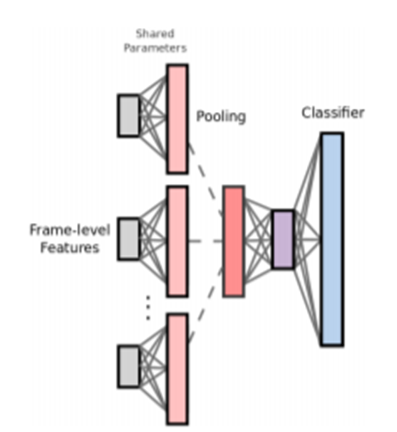
\includegraphics[width=0.5\textwidth]{chapter2/images/DBoF.png}
				\caption{โครงสร้างของโมเดล DBoF}
    			\label{fig:DBoF}
		\end{figure}
		\\ หลักการคล้ายๆกับ Deep Bag of Words โดยที่จะสุ่มเฟรม มา k เฟรม โดยที่แต่ละเฟรมเป็น N dimension input มาผ่าน fully connected ที่มี M units (M > N) และใช้ RELU activations แล้วทำ batch normalization ก่อนจะนำมารวมด้วย max pooling โดยที่ทั้งโครงข่ายใช้ Stochastic  Gradient Descent(SGD) 
		\item Long short-term memory(LSTM)
		\\ ในบทความ \footnote{YouTube-8M,https://arxiv.org/pdf/1609.08675.pdf} นี้ได้ใช้ LSTM แบบเดียวกับของ Beyond Short Snippets: Deep Networks for Video Classification \footnote{AVA,https://arxiv.org/pdf/1705.08421.pdf} แต่เนื่องจาก YouTube-8M นั้นผ่านการทำ preprocess มาแล้วทำให้ไม่สามารถใช้ raw video frame ได้ จึงทำได้เฉพาะ LSTM และ softmax layer เท่านั้น ตามรูปที่ \ref{fig:BSS}
		\begin{figure}[!ht]
			\centering
			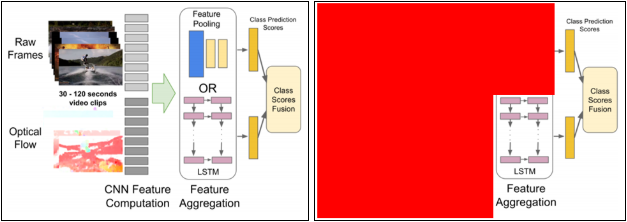
\includegraphics[width=1\textwidth]{chapter2/images/BSS.png}
				\caption{(ซ้าย) โครงสร้างจาก Beyond Short Snippets: Deep Networks for Video Classification, (ขวา) ส่วนที่สามารถใช้งานกับ YouTube-8M ได้}
    			\label{fig:BSS}
		\end{figure}
	\end{enumerate}
	\item คุณลักษณะระดับวิดีโอ (Video-level feature)
	\begin{enumerate}
		\setlength\itemsep{-0.25em}
		\item Video-level representation 
		\\ ในบทความ \footnote{YouTube-8M,https://arxiv.org/pdf/1609.08675.pdf}นี้ได้สำรวจวิธีการแยกเวกเตอร์คุณลักษณะระดับวิดีโอความยาวคงที่จากคุณลักษณะระดับเฟรมซึ่งการทำแบบนี้ทำให้ได้ประโยชน์ 3 ข้อ คือ 1) โมเดลทั่วไปที่ไม่ใช่ neural network สามารถนำไปใช้งานได้  2) ขนาดข้อมูลเล็กลง  3) เหมาะกับการนำไปสร้างโมเดล domain adaptive มากขึ้น
		\begin{enumerate}
			\setlength\itemsep{-0.25em}
			\item First, Second order and ordinal statistic
			\\ จากคุณลักษณะในระดับเฟรม $x_{1:F_{v}}^{v}$ โดยที่ $x_{j}^{v}$ คือคุณลักษณะระดับเฟรมในเฟรมที่ $j$ ของวิดีโอ $v$ และ $F_{v}$ คือจำนวนเฟรมทั้งหมดของวิดีโอ $v$ ทำการหาค่าเฉลี่ย $\mu_{v}$ และส่วนเบี่ยงเบนมาตรฐาน $\sigma_{v}$ พร้อมทั้งดึง ordinal statistics 5 อันดับแรกของแต่ละ dimension K ออกมา $Top_{k}(x^{v}(j)_{1:F_{v}})$ จะทำให้ได้เวคเตอร์คุณลักษณะ(feature-vector) $\varphi_{1:F_{v}}^{v}$ ของวิดีโอเป็นดังนี้ \\
			\centerline{$\varphi_{1:F_{v}}^{v} = \begin{bmatrix}
								\mu_{1:F_{v}}^{v}\\ 
								\sigma_{1:F_{v}}^{v}\\ 
								Top_{k}(x^{v}(j)_{1:F_{v}})
								\end{bmatrix}$}
			\item Feature normalization \\
			ก่อนที่จะทำการสร้าง one vs all classifiers แต่ละตัวนั้นได้ทำ normalization เวกเตอร์คุณลักษณะ $\varphi_{1:F_{v}}^{v}$ จากนั้นนำค่าเฉลี่ย $\mu_{v}$ ออกแล้วใช้ PCA ในการลด มิติของข้อมูล ซึ่งการทำแบบนี้นั้นทำให้การสร้างโมเดลเป็นไปได้เร็วขึ้น
		\end{enumerate}
		โดยการสร้างโมเดลด้วย video-level presentation นั้น บทความ \footnote{YouTube-8M,https://arxiv.org/pdf/1609.08675.pdf} นี้ได้หยิบมาทดสอบ 3 อัลกอริทึม
		\item Model training algorithm approaches 
		\begin{enumerate}
			\setlength\itemsep{-0.25em}
			\item Logistic Regression
			\item Hinge Loss
			\item Mixture of Experts (MoE)
		\end{enumerate}
		\item Evaluation metrics
		\begin{enumerate}
			\setlength\itemsep{-0.25em}
			\item Mean Average Precision (mAP)
			\item Hit@k
			\item Precision at equal recall rate (PERR)
		\end{enumerate}
	\end{enumerate}
	\item Results
	\begin{enumerate}
		\setlength\itemsep{-0.25em}
		\item Baseline on YouTube-8M dataset
\begin{table}[!ht]
\centering
\begin{tabular}{|c|c|c|c|c|}
		\hline
		{Inpute Features}&{Modeling Approach}&{mAP}&{Hit@1}&{(PERR)}\\
		\hline
		Frame-level, $(x_{1:F_{v}}^{v})$	& Logistic + Average		& 11.0		& 50.8		& 42.2					\\
		Frame-level, $(x_{1:F_{v}}^{v})$	& Deep Bag of Frames	& 26.9		& 62.7		& 55.1					\\
		Frame-level, $(x_{1:F_{v}}^{v})$	& LSTM				& 26.6		& 64.5		& 57.3					\\
		\hline
		Video-level, $\mu$					& Hinge loss					& 26.6		& 64.5		& 57.3				\\
		Video-level, $\mu$					& Logistic Regression				& 26.6		& 64.5		& 57.3				\\
		Video-level, $\mu$					& Mixture-of-2-Expert				& 26.6		& 64.5		& 57.3				\\
		Video-level, $\mu ; \sigma ; Top_{5} $	& Mixture-of-2-Expert				& 26.6		& 64.5		& 57.3				\\
		\hline
	\end{tabular}
	\caption{ประสิทธิภาพของโมเดลที่สร้างจาก YouTube-8M ด้วยวิธีต่างๆตามหัวข้อที่ 1 และ 2 โดยแถวที่ 1 คือ frame-level โมเดลและแถวที่ 2 คือ video-level โมเดล}
	\label{tab: ประสิทธิภาพของโมเดลที่สร้างจาก YouTube-8M}
\end{table}
\\
		จากตารางที่ \ref{tab: ประสิทธิภาพของโมเดลที่สร้างจาก YouTube-8M} จะเห็นว่าการทำ video-level features จากการหาค่าเฉลี่ยของ frame-level features แล้วสร้างโมเดลด้วย Hinge loss หรือ โมเดล Logistic Regression นั้นสามารถเพิ่มประสิทธิภาพได้ไม่น้อย และจากการทดลองทำให้เห็นว่า LSTM ที่มีความลึก 2 layers นั้นสามารถทำให้ผลลัพธ์เป็น state-of-the-art ในขณะนั้นได้ เนื่องจากในขณะที่ DBoF นั้นไม่ได้สนใจลำดับของเฟรม แต่ LSTM ใช้ state information เพื่อคงลำดับของเฟรมเอาไว้
\\
\\
		 LSTM นั้นดีที่สุดยกเว้น mAP, เนื่องจาก one-vs-all binary MoE classifier นั้นมีประสิทธิภาพดีกว่า, LSTM สามารถเพิ่มประสิทธิภาพบน Hit@1 และ PERR ได้เนื่องจากความสามารถในการเรียนรู้ความสัมพันธ์ระยะยาวในโดเมนของเวลา
		\clearpage
		\item Transfer learning video-level presentation from YouTube-8M to Sports-1M dataset
\begin{table}[!ht]
\centering
\begin{tabular}{|c|c|c|c|}
		\hline
		{Approach}&{mAP}&{Hit@1}&{(Hit@1)}\\
		\hline
		Logistic Regression ($\mu$)					& 58.0		& 60.1		& 79.6					\\
		Mixture-of-2-Expert ($\mu$)					& 59.1		& 61.5		& 80.4					\\
		Mixture-of-2-Expert ([$\mu ; \sigma ; Top_{5}$		& 61.3		& 63.2		& 82.6					\\
		LSTM									& 66.7		& 64.9		& 85.6					\\
		+Pretrained on YT-8M							& 67.6		& 65.7		& 86.2					\\
		\hline
		Hierarchical 3D Convolution						& -			& 61.0		& 80.0					\\
		Stacked 3D Convolutions						& -			& 61.0		& 85.0					\\
		LSTM with Optical Flow and Pixels				& -			& 73.0		& 91.0					\\
		\hline
	\end{tabular}
	\caption{ประสิทธิภาพของโมเดลเมื่อถูก transfer learning ด้วยชุดข้อมูล Sports-1M โดยใช้ video-level presentation}
	\label{tab: transfer learning}
\end{table}
\\
		จากตารางที่  \ref{tab: transfer learning} จะเห็นว่าโมเดล LSTM ที่ถูก pretrained จาก YouTube-8M นั้นมีประสิทธิภาพที่ดีกว่า ยกเว้น LSTM with Optical Flow and Pixels ที่มีการใช้ข้อมูลการเคลื่อนไหว(optical flow) ในการสร้างโมเดลด้วย
\\

		\item Transfer learning video-level presentation from YouTube-8M to ActivityNet dataset
\begin{table}[!ht]
\centering
\begin{tabular}{|c|c|c|c|}
		\hline
		{Approach}&{mAP}&{Hit@1}&{(Hit@1)}\\
		\hline
		Mixture-of-2-Expert ($\mu$)					& 69.1		& 68.7		& 85.4					\\
		+Pretrained PCA on YT-8M						& 74.1		& 72.5		& 89.3					\\
		Mixture-of-2-Expert ([$\mu ; \sigma ; Top_{5}$		& NO			& 74.2		& 72.3					\\
		+Pretrained PCA on YT-8M						& 77.6		& 74.9		& 91.6					\\
		LSTM									& 57.9		& 63.4		& 81.0					\\
		+Pretrained on YT-8M							& 75.6		& 74.2		& 92.4					\\
		\hline
		Ma, Bargal et al.								& 53.8		& -			& -						\\
		Heilbron et al.								& 43.0		& -			& -						\\
		\hline
	\end{tabular}
	\caption{ประสิทธิภาพของโมเดลเมื่อถูก transfer learning ด้วยชุดข้อมูล ActivityNet โดยใช้ video-level presentation}
	\label{tab: transfer learning ActivityNet}
\end{table}
\\
		จากตารางที่ \ref{tab: transfer learning ActivityNet} จะเห็นว่าโมเดลที่ถูก pretrained จาก YouTube-8M นั้นมีประสิทธิภาพที่ดีขึ้นมากเมื่อเทียบกับ benchmark ก่อนหน้า
	\end{enumerate}
\end{enumerate}

\subsubsection*{3. ปัญหาที่พบ}
เนื่องจากว่า YouTube-8M นั้นมีจำนวนข้อมูลที่เยอะมาก ทำให้ไม่สามารถตรวจสอบได้ทั้งหมดว่า ground-truth ของแต่ละวิดีโอนั้นมีความถูกต้องมากน้อยขนาดไหน ทำให้อาจเกิดข้อผิดพลาดได้ (ปัจจุบัน ปี 2019 YouTube-8M ได้มีการตรวจสอบข้อมูลอีกครั้ง เพื่อเพิ่มประสิทธิภาพของชุดข้อมูลซึ่งทำให้ปัจจุบันจำนวนข้อมูล และจำนวน category นั้นจะลดน้อยลงจากข้อมูลที่ใช้อ้างอิงในบทความ \footnote{YouTube-8M,https://arxiv.org/pdf/1609.08675.pdf} ข้างต้นที่ได้กล่าวมา)







%\clearpage
%AVA\textsuperscript{\cite{AVA}} คือ ชุดข้อมูลที่รวบรวมวิดิโอที่มีความยาว 15 นาที ถูกแบ่งด้วยความถี่ 1 hz (900 keyframes) จากในภาพยนต์โดยยึดการกระทำของมนุษย์เป็นศูนย์กลาง
เพื่อใช้สำหรับสร้างโมเดลที่เข้าใจกิจกรรมของมนุษย์ในวิดิโอว่ามนุษย์กำลังทำอะไรอยู่ ซึ่งข้อดีของ AVA คือ ชุดข้อมูลจะมีคำกำกับเป็นแบบทวิคำกำกับ (multiple label)
และคำกำกับของ AVA มีจำนวน 80 ประเภท สามารถแบ่งได้เป็นสามหมวดหมู่คือ ท่าทาง (Pose), ปฏิสัมพันธ์กับวัตถุ (Interaction with object) 
และปฏิสัมพันธ์กับบุคคล (Interaction with people) ซึ่งสามารถมีคำกำกับได้มากสูงสุดถึง 7 คำกำกับ
\begin{enumerate}
	\item {รายละเอียดชุดข้อมูล}
	\begin{enumerate}
		\item ขั้นตอนการเก็บข้อมูลสำหรับการทำชุดข้อมูลมีขั้นตอนการทำ 5 ขั้นดังนี้
		\begin{enumerate}
			\item การสร้างคำศัพท์การกระทำจะมีหลักการ 3 ข้อในการรวบรวมคำศัพท์ดังนี้
			\begin{enumerate}
				\item เก็บรวบรวมคำศัพท์ทั่วไปที่เกิดขึ้นในชีวิตประจำวัน
				\item จะต้องมีเอกลักษณ์สามารถเห็นได้ชัดเจน เช่น การถือของ
				\item กำหนดรูปแบบของคำศัพท์ขึ้นมา และใช้ความรู้จากชุดข้อมูลอื่นในการทำให้ได้หมวดหมู่การกระทำของมนุษย์ที่ครอบคลุม
			\end{enumerate}
			\item ภาพยนต์และส่วนที่เลือกมาใช้ทำชุดข้อมูล AVA ทั้งหมดจะถูกนำมาจาก YouTube โดยเริ่มจากการรวบรวมเอารายชื่อของนักแสดงที่มีชื่อเสียง
			ซึ่งจะมีความหลากหลายของเชื้อชาติรวมกันอยู่ วิดีโอที่ถูกคัดเลือกจะมีเกณฑ์ดังนี้
			\begin{enumerate}
				\item วิดีโอต้องอยู่ในหมวด ภาพยนต์ และละครโทรทัศน์
				\item วิดีโอจะต้องมีความยาวมากกว่า 30 นาที
				\item เผยแพร่มาแล้วเป็นระยะเวลาอย่างน้อย 1 ปี
				\item มีจำนวนยอดคนดูมากกว่า 1,000 ครั้ง
				\item ละเว้นวิดีโอบางประเภท เป็นภาพขาว-ดำ มีความละเอียดต่ำ การ์ตูน หรือวิดีโอเกม
			\end{enumerate}
			\item การสร้างกรอบสี่เหลี่ยมครอบมนุษย์ที่อยู่ภายในภาพประกอบด้วย 2 ขั้นตอน
			\begin{enumerate}
				\item สร้างกรอบสี่เหลี่ยมโดยใช้โมเดลปัญญาประดิษฐ์ faster RCNN สำหรับการตรวจจับมนุษย์
				\item ใช้มนุษย์ในการตรวจสอบและแก้ไขกรอบสี่เหลี่ยมที่ผิดพลาด
			\end{enumerate}	
			\item การติดตามตำแหน่งของบุคคล\\
			ทำการติดตามตำแหน่งของบุคคลที่อยู่ในช่วงเวลาเดียวกันด้วยใช้วิธีการแทร็กโดยยึดมนุษย์เป็นศูนย์กลาง โดยการคำนวณค่าความใกล้เคียงกันระหว่างบุคคล 
			โดยใช้ person embedding (ใช้โครงข่ายประสาทเทียมในการหาฟีเจอร์ขั้นสูงและใช้เมทริกซ์ในการหาความสัมพันธ์ของแต่ละคน) จากนั้นจะใช้อัลกอริทึม Hungarian distance (อัลกอริทึ่มสำหรับการหาข้อเสนอที่ดีที่สุด) ในการหาตัวเลือกคู่ของกรอบสี่เหลี่ยมที่ดีที่สุด
			\item การสร้างคำกำกับคุณลักษณะ\\
			การสร้างคำกำกับของการกระทำจะถูกสร้างขึ้นโดยมนุษย์ ซึ่งผู้วิจัยจะใช้โปรแกรมสำหรับช่วยเหลือในการสร้างคำกำกับคุณลักษณะ โดยสามารถกำหนดคำกำกับของการกระทำได้สูงสุดถึง 7 คำต่อ 1 กรอบสี่เหลี่ยม นอกจากนั้นสามารถตั้งสถานะเนื้อหาที่ไม่เหมาะสม หรือ กรอบสี่เหลี่ยมที่ผิดพลาดได้อีกด้วย ซึ่งในทางปฎิบัติเพื่อลดโอกาสที่จะเกิดข้อผิดพลาด จึงแบ่งขั้นตอนในการสร้างคำกำกับออกเป็น 2 ขั้นตอนดังนี้
			\begin{enumerate}
				\setlength\itemsep{-0.25em}
				\item สร้างข้อเสนอสำหรับคำกำกับของการกระทำ
				\item ข้อเสนอจะถูกตรวจสอบข้อเสนอที่ได้จากขั้นตอนแรก ซึ่งจะใช้มนุษย์ในการตรวจสอบ 3 คน โดยคำกำกับจะต้องถูกตรวจสอบด้วยผู้ตรวจสอบอย่างน้อย 2 คน จึงจะถูกยึดเป็นคำกำกับหลัก
			\end{enumerate}
		\end{enumerate}
	\end{enumerate}
	\item {โมเดลปัญญาประดิษฐ์}
	\begin{enumerate}
		\item โมเดลปัญญาประดิษฐ์ที่งานวิจัยนี้ใช้ คือ two stream variant ซึ่งจะทำการประมวลผลทั้ง RGB flow และ optical flow 
		โดยเป็นโครงสร้างของ faster RCNN ที่นำ Inception network เข้ามาใช้
		\item เครื่องมือที่ใช้วัดผลสำหรับงานวิจัยนี้ คือค่า IoU และ 3D IoUs 
		\begin{enumerate}
			\item ค่า IoU คือค่าที่ใช้วัดความสอดคล้องระหว่างสองกรอบสี่เหลี่ยม(กรอบสี่เหลี่ยมจริงของเฟรม และ กรอบสี่เหลี่ยมที่ทำนายขึ้นมา) ซึ่งใช้สำหรับการวัดผลระดับเฟรม 
			\item ค่า 3D IoUs คือค่าที่ใช้วัดความสอดคล้องระหว่างกรอบสี่เหลี่ยมภายใน 2 วิดีโอ ซึ่งใช้สำหรับการวัดผลระดับวิดีโอ โดยเทียบกันระหว่างกรอบสี่เหลี่ยมจริงในช่วงของเฟรมที่ต่อกัน (ground-truth tubes) และ กรอบสี่เหลี่ยมที่ทำนายขึ้นมาในช่วงของเฟรมที่ต่อกัน (linked detection tubes) 
		\end{enumerate}
		\item ประสิทธิภาพของโมเดลปัญญาประดิษฐ์ในปัจจุบัน
		\\ข้อมูลโมเดลปัญญาประดิษฐ์ที่นำมาทดสอบ
		\begin{enumerate}				
			\item Actionness\textsuperscript{\cite{actioness}} เป็นการหาความน่าจะเป็นของการกระทำ โดยใช้โครงสร้างของ hybrid fully convolutional network (HFCN) hybrid fully เป็นโครงสร้างที่ประกอบด้วยโครงข่ายประสาทเทียม 2 ชนิด คือ
			\begin{enumerate}
				\item Appearance-FCN (A-FCN) คือ โครงข่ายประสาทเทียมที่นำมาใช้แสดงลักษณะของวัตถุ(ตำแหน่งวัตถุ, ความตื้นลึกวัตถุ) ที่ปรากฎบนรูป RGB1
				\item MotionFCN (M-FCN) คือ โครงข่ายประสาทเทียมที่แยกการเคลื่อนไหวจากข้อมูลของ optical flow
			 \end{enumerate}
			\item Peng without MR, Peng with MR (Multi-region two-stream R-CNN)\textsuperscript{\cite{peng}} เป็นโมเดลปัญญาประดิษฐ์ที่ใช้สำหรับตรวจจับวิดีโอในชีวิตจริง ซึ่งพื้นฐานของโมเดลนี้เป็น Faster R-CNN โดยโมเดลนี้มีกระบวนการ 3 กระบวนการคือ
			\begin{enumerate}
					\item สร้างข้อเสนอพื้นที่ที่มีการเคลื่อนไหว
					\item สะสม Optical flow จากเฟรมหลายๆเฟรม เพื่อนำไปปรับปรุงการตรวจจับการกระทำ
					\item นำพื้นที่หลายๆส่วนมาวิเคราะห์ผ่านโมเดล Faster R-CNN
			\end{enumerate}
			\item ACT Action Tubelet Detector\textsuperscript{\cite{act}} เป็นการระบุตำแหน่งของการกระทำที่มีระยะเวลาๆสั้นๆ ซึ่งใช้วิธีการตรวจจับระดับเฟรม และ ใช้การติดตามตำแหน่งในการเชื่อมระหว่างเฟรมปัจจุบันไปยังเฟรมถัดไป. ACT ถูกสร้างต่อจาก SSD framework และ ใช้คอนโวลูชันในการสกัดคุณลักษณะในแต่ละเฟรมซึ่งการคิดคะแนนและความน่าจะเป็นของหมวดหมู่จะคิดจากการนำคุณลักษณะเรียงต่อกัน และ หาข้อมูลจากลำดับข้อมูลนั้น
		\end{enumerate}
		จากการทดสอบการเทียบโมเดลปัญญาประดิษฐ์ของงานวิจัยนี้และวิธีการอื่นๆ โดยนำไปทดสอบกับชุดข้อมูลวิดีโอ JHMDB และ UCF101-24 ได้ผลลัพธ์ออกมาดังนี้
			\begin{table}[!ht]
				\centering
				\begin{tabular}{|c|c|c|c|}
					\hline
					{Frame-mAP}&{JHMDB (mAP)}&{UCF101-24 (mAP)}								\\
					\hline
					Actionness 			& 39.9				& 	-						\\
					Peng w/o MR			& 56.9				& 64.8						\\
					Peng w/  MR 			& 58.5				& 65.7						\\
					ACT					& 65.7				& 69.5						\\
					\hline
					2 stream(Our approach)		& \textbf{73.3}		& \textbf{76.3}				\\
					\hline
				\end{tabular}
				\caption{ผลการทดลองของวิธีต่างๆบนคุณลักษณะระดับเฟรม}
				\label{tab: transfer learning}
			\end{table}
		\item ปัญหาที่พบ
		ในปัจจุบันยังไม่มีโมเดลปัญญาประดิษฐ์ที่ทดสอบด้วยชุดข้อมูล AVA และได้ผลการทำงานที่ดี เนื่องจากชุดข้อมูลนี้สนใจการกระทำของมนุษย์ที่มีรายละเอียดเล็กๆน้อยๆ 
		ทำให้ยากต่อการทำนายสำหรับโมเดลปัญญาประดิษฐ์
	\end{enumerate}
\end{enumerate}
%\clearpage
%Moments in time\textsuperscript{\cite{monfort2019moments}} คือชุดข้อมูลที่ใช้มนุษย์ในการกำกับข้อมูลทั้งหมดให้กับวิดีโอสั้นถึง 1 ล้านวิดีโอ 
และมีจำนวนกิจกรรมหรือการกระทำต่างกัน 339 หมวดหมู่ โดยแต่ละวิดีโอจะมีความยาวอยู่ที่ 3 วินาที เนื่องจากเป็นเวลาเฉลี่ยที่มนุษย์ใช้ในการเข้าใจกับเหตุการณ์ที่เกิดขึ้น
(human working memory) รูปแบบของชุดข้อมูลจะมีอยู่ทั้งหมดอยู่ 3 รูปแบบ ได้แก่ ภาพนิ่ง (spatial) เสียง (auditory) และการเคลื่อนไหว (temporal) 
นอกจากนี้ชุดข้อมูลนี้นั้นไม่รวบรวมเพียงแค่การกระทำของมนุษย์เท่านั้น ยังรวมไปถึง สัตว์ สิ่งของ และปรากฏการณ์ธรรมชาติ ทำให้ชุดข้อมูลนี่เป็นการท้าทายรูปแบบใหม่เพราะด้วยข้อมูลที่มีความซับซ้อนมากขึ้น
\begin{enumerate}
	\item {รายละเอียดชุดข้อมูล}
	\begin{enumerate}
		\setlength\itemsep{-0.25em}
		\item เป้าหมายของชุดข้อมูล : สนใจเหตุการณ์ที่เกิดขึ้นในวิดีโอ เช่น การกระทำของคนหรือสัตว์ เหตุการณ์ และปรากฎการณ์ธรรมชาติ 
		\item จำนวนของวิดีโอ : มากกว่า 1,000,000 วิดีโอ
		\item ความยาวเฉลี่ยของแต่ละวิดีโอ : 3 วินาที
		\item จำนวนของหมวดหมู่ : 339 หมวดหมู่
		\item วิธีการเก็บรวบรวมข้อมูล
	\begin{enumerate}
		\item เริ่มจากการรวบรวมคำที่ใช้อยู่ทั่วไปในชีวิตประจำวันมา 4,500 คำจาก VerbNet\textsuperscript{\cite{Schuler:2005:VBC:1104493}} เว็บไซต์ที่เก็บรวบรวมคำกิริยาภาษาอังกฤษขนาดใหญ่ 
		จากนั้นนำมาแบ่งกลุ่มคำที่มีความหมายใกล้เคียงกันโดยใช้คุณลักษณะจาก Propbank\textsuperscript{\cite{Zaghouani:2010:RAP:1868720.1868756}} และ
		FrameNet\textsuperscript{\cite{Baker:1998:BFP:980451.980860}} โดยเก็บข้อมูลเป็นแบบเวกเตอร์คุณลักษณะฐานสอง (binary feature vector) 
		ซึ่งถ้าคำใดมีความเกี่ยวข้องกันทางคุณลักษณะก็จะให้ค่าเป็น 1 ถ้าไม่เกี่ยวข้องกันจะให้ค่าเป็น 0 จากนั้นจึงใช้วิธี k-means clustering ในการแบ่งกลุ่ม 
		เมื่อแบ่งกลุ่มแล้วจากนั้นจะเลือกคำจากในแต่ละกลุ่มนั้น โดยคำที่เลือกมานั้นจะเป็นคำที่ใช้บ่อยที่สุดในกลุ่มนั้น และลบคำนั้นออกจากกลุ่มอื่นๆทั้งหมด (คำๆหนึ่งสามารถอยู่ได้หลายกลุ่ม) 
		จากนั้นจะทำกระบวนการนี่ไปเรื่อยๆ แต่คำที่เลือกมาจะต้องไม่มีความหมายคลุมเครือ หรือเป็นสิ่งที่ไม่สามารถมองเห็นหรือได้ยินได้ และต้องไม่มีความหมายเหมือนกับคำที่เคยเลือกมาก่อน 
		จนสุดท้ายแล้วได้ออกมาที่ 339 หมวดหมู่
		\item ต่อมาทำการหาชุดข้อมูลวิดีโอโดยจะตัดออกมาเพียง 3 วินาทีที่เกี่ยวข้องกับคำใน 339 หมวดหมู่ที่เลือกมาจากวิดีโอแหล่งต่างกัน 10 แหล่ง 
		การตัดวิดีโอนั้นจะไม่ใช้พวก Video2Gif (โมเดลที่ระบุตำแหน่งของสิ่งที่น่าสนใจในวิดีโอ) เพราะจะทำให้เกิดอคติขึ้นจะเกิดขึ้นตอนสร้างโมเดล ดังนั้นจึงใช้มนุษย์ในการตัดวิดีโอ จากนั้นจะทำการส่งข้อมูลของคำ
		และวิดีโอที่ตัดไปยัง Amazon Mechanical Turk (AMT หรือตลาดแรงงาน) เพื่อทำการสร้างคำกำกับโดยพนักงานของ AMT ทำให้ได้ 64 วิดีโอที่เกี่ยวข้องกับคำหนึ่ง 
		และอีก 10 วิดีโอที่มีคำกำกับอยู่แล้ว โดยวิดีโอที่มีคำกำกับอยู่แล้วนั้นถ้าพนักงานของ AMT ตอบเหมือนกันเกิน 90\% ถึงจะนำเข้าไปรวมกับชุดข้อมูลส่วนอีก 64 วิดีโอ
		ถ้าเป็นชุดข้อมูลสำหรับสร้างโมเดลจะต้องผ่านพนักงานของ AMT อย่างน้อย 3 ครั้ง และต้องมีคำกำกับเหมือนกัน 75\% ขึ้นไปถึงจะถือว่าเป็นคำกำกับที่ถูกต้อง 
		ถ้าเป็นชุดข้อมูลสำหรับตรวจคำตอบ และชุดข้อมูลสำหรับทดสอบจะต้องผ่านพนักงานของ AMT อย่างน้อย 4 ครั้ง และต้องมีคำกำกับเหมือนกัน 85\% ขึ้นไป 
		เหตุผลที่ไม่ตั้งเกณฑ์ไว้ที่ 100\% เพราะจะทำให้วิดีโอนั้นยากเกินไปที่จะทำให้สามารถจำการกระทำได้	
	\end{enumerate}
\end{enumerate}
	\item การเตรียมข้อมูล
		\begin{enumerate}
			\item ชุดข้อมูลสำหรับสร้างโมเดลจะมี 802,264 วิดีโอ และมีวิดีโอในแต่ละหมวดหมู่อยู่ที่ 500 ถึง 5,000 วิดีโอ
			\item ชุดข้อมูลสำหรับตรวจคำตอบจะมี 33,900 วิดีโอ และมีวิดีโอในแต่ละหมวดหมู่อยู่ที่ 100 วิดีโอ
			\item แยกเฟรม RGB ออกมาจากวิดีโอ และทำการเปลี่ยนขนาดให้เป็น 340\texttimes256  pixel
			\item ใช้อัลกอริทึม TVL1 optical flow จาก Opencv เพื่อลดข้อมูลรบกวนที่จะเกิดขึ้น
			\item ทำการแปลงค่าที่อยู่ใน optical flow ให้เป็นเลขจำนวนเต็มเพื่อทำให้การคำนวณนั้นเร็วยิ่งขึ้น
			\item ปรับค่า displacement ใน optical flow ให้ค่าสูงสุดเป็น 15 ต่ำสุดเป็น 0 และทำการปรับขนาดให้เป็นช่วง 0 - 255
			\item เก็บข้อมูลออกมาในรูปแบบของภาพขาวดำเพื่อลดพื้นที่ในการเก็บข้อมูล
			\item แก้ปัญหาเรื่องการเคลื่อนไหวของกล้องด้วยการนำค่าเฉลี่ยของเวกเตอร์ไปลบกับ displacement
			\item สุดท้ายจะเป็นสุ่มตัดภาพออกมาเพื่อเพิ่มจำนวนข้อมูล
		\end{enumerate}
	\item {โมเดลปัญญาประดิษฐ์}
	\begin{enumerate}
		\item ในงานวิจัยนี้มีการทดสอบโมเดลปัญญาประดิษฐ์หลายรูปแบบ โดยโมเดลปัญญาประดิษฐ์ที่มีประสิทธิภาพการทำงานที่ดีที่สุด 5 ลำดับแรกมีดังนี้
			\begin{enumerate}
				\item SVM มีรูปแบบข้อมูลที่ป้อนเข้า คือ เฟรมที่ต่อเนื่อง (spatial) + เฟรมเดี่ยว (temporal) + ข้อมูลเสียง (auditory) 	
				\item I3D มีรูปแบบข้อมูลที่ป้อนเข้า คือ เฟรมที่ต่อเนื่อง + เฟรมเดี่ยว
				\item TRN-Multiscale มีรูปแบบข้อมูลป้อนเข้า คือ เฟรมที่ต่อเนื่อง + เฟรมเดี่ยว
				\item TSN-2stream มีรูปแบบข้อมูลป้อนเข้า คือ เฟรมที่ต่อเนื่อง + เฟรมเดี่ยว
				\item ResNet50-ImageNet	มีรูปแบบข้อมูลป้อนเข้า คือ เฟรมที่ต่อเนื่อง
			\end{enumerate}
		\item เครื่องมือที่ใช้วัดผลงานวิจัยนี้
			\begin{enumerate}
				\item Classification accuracy Top-1, Top-5
			\end{enumerate}
		\item ประสิทธิภาพของโมเดลปัญญาประดิษฐ์ในปัจจุบัน
			\begin{enumerate}
				\item ทำการทดสอบด้วยวิธี cross dataset transfer โดยการนำโมเดล ResNet50 I3D ที่สร้างด้วยชุดข้อมูล Kinetics และ Moments in Time 
				แล้วนำทั้ง 2 โมเดลไปทดสอบกับชุดข้อมูลอื่น โดยจะปรับอัตราความถี่ของเฟรม (frame rate) ของวิดีโอให้เป็น 5 fps
				\begin{table}[!ht]
					\centering
					\begin{tabular}{|c|c|c|c|}
						\hline
						{Pretrained}&\multicolumn{3}{c|}{Fine-Tuned}\\
						\cline{2-4}
						{}								& UCF-101			& HMDB-51			& Something Something			\\
						\hline
						\multirow{2}{*}{Kinetics}		& Top-1 : 92.6		& Top-1 : 62.0		& Top-1 : 48.6		\\
						{}								& Top-5 : 99.2		& Top-5 : 88.2		& Top-5 : 77.9		\\
						\hline
						\multirow{2}{*}{Moments}		& Top-1 : 91.9		& Top-1 : 65.9		& Top-1 : 50.0		\\
						{}								& Top-5 : 98.6		& Top-5 : 89.3		& Top-5 : 78.8		\\
						\hline
					\end{tabular}
					\caption{ประสิทธิภาพของโมเดล Resnet50 I3D ที่ใช้ชุดข้อมูล Kinetics และ Moments in Time}
					\label{tab: Data transfer performance ของโมเดล Resnet50 I3D}
				\end{table}
				\item จะเห็นได้ว่า Kinetics ให้ผลลัพธ์ที่ดีกว่าใน UCF-101 เพราะว่ามีหมวดหมู่ที่ตรงกันอยู่หลายอย่าง ในขณะที่ HMDB-51 นั้นมีการรวบรวมข้อมูลจากหลายแหล่ง 
				และมีจำนวนหมวดหมู่ที่หลากหลายจึงทำให้มีความใกล้เคียงกับตัวข้อมูลของ Moments in Time ดังนั้นจึงเทียบผลลัพท์จาก Something Something 
				ซึ่งจะทำให้เห็นว่า Moments in Time มีประสิทธิภาพที่ดีกว่าและวิดีโอที่มีความยาวมากกว่า 3 วินาทีจะไม่ส่งผลกระทบกับประสิทธิภาพของ Moments in Time
		\end{enumerate}
	\end{enumerate}
	\item {ปัญหาที่พบ}\\
	ผลลัพธ์จากการทำนายด้วยโมเดลถ้าผ่านภาพที่มีรายละเอียดเยอะจะทำให้การ ทำนายโอกาสผิดนั้นค่อนข้างสูง ซึ่งปัญหานี่สามารถทำให้เกิดน้อยลงด้วยการนำวิธี 
	class activation mapping (CAM) จะเป็นการเน้นภาพในส่วนที่มีข้อมูลมากที่สุดและทำนายผลออกมา แต่ก็ยังมีจุดที่เป็นปัญหาอยู่ เช่น 
	การกระทำที่เกิดขึ้นเร็วมากจะทำให้การทำนายนั้นมีโอกาสผิดสูงขึ้น
\end{enumerate}		

\section{ทฤษฎีที่เกี่ยวข้อง}
\subsection{Optical flow}
Optical flow \footnote{Optical flow,shorturl.at/mrtEZ}  คือรูปแบบของการเคลื่อนที่ของวัตถุในรูปภาพระหว่างภาพซึ่งอาจจะการจากเคลื่อน ที่ของวัตถุหรือตัวกล้อง ออกมาในรูปแบบของ เวกเตอร์(vector) 2 มิติ โดยที่เวกเตอร์แต่ละตัวจะแสดงถึงทิศทางการเคลื่อนที่ระหว่างภาพดังรูปด้านล่าง

\begin{figure}[!ht]
	\centering
	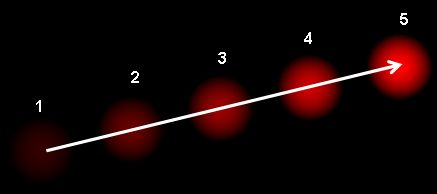
\includegraphics[width=1\textwidth]{chapter2/images/vector_optical.png}
		\caption{ตัวอย่างการเคลื่อนที่ของลูกบอล}
    	\label{fig:vector_optical}
\end{figure}

จากรูปภาพจะแสดงให้เห็นถึงการเคลื่อนที่ของลูกบอลของภาพที่ต่อเนื่องกัน 5 ภาพโดยที่ลูกศรแสดงถึงทิศทางการเคลื่อนที่ของเวกเตอร์
\\
\clearpage
\par
การทำงานของ optical flow อยู่บนสมมติฐานหลายประการได้แก่
\begin{enumerate}
	\setlength\itemsep{-0.25em}
	\item ความเข้มของพิกเซล(pixel) ของวัตถุจะไม่เปลี่ยนแปลงระหว่างภาพที่ต่อเนื่องกัน
	\item พิกเซลที่อยู่ใกล้กันจะมีการเคลื่อนไหวที่คล้ายกัน
\end{enumerate}

เมื่อพิจารณาพิกเซล I(x,y,t) จากภาพแรกจะเคลื่อนไหวเป็นระยะทาง (dx,dy) ไปยังภาพต่อไปหลังจากผ่านไปแล้ว dt เวลา ดังนั้นเนื่องจาก พิกเซล เหล่านี้เหมือนกันและความเข้มไม่มีการเปลี่ยนแปลง จึงทำให้พูดได้ว่า
\\
\centerline{$I(x,y,t) = I(x + dx, y + dy, t + dt)$}		\\
\centerline{$I$ คือ พิกเซลจากภายในภาพ}			\\
\centerline{$x$ คือ ตำแหน่งของพิกเซล ในแกน x} 		\\
\centerline{$dx$ คือ ระยะทางที่เคลื่อนที่ในแกน x} 		\\
\centerline{$y$ คือตำแหน่งของพิกเซลในแกน y} 		\\
\centerline{$dy$ คือ ระยะทางที่เคลื่อนที่ในแกน y}		\\
\centerline{$t$ คือ เวลา}						\\
\centerline{$dt$ คือ ระยะเวลาที่เปลี่ยนไประหว่างภาพ} 	\\

จากนั้นใช้การประมาณค่าของ taylor series ทางฝั่งขวามือและ ลบค่า common term และหารด้วย dt เพื่อให้ได้สมการดังต่อไปนี้
\\
\centerline{$f_{x}u + f_{y}v + f_{t} $}				\\
โดยที่
\\
\centerline{$f_{x} = \frac{\delta f}{\delta x} ; f_{y} = \frac{\delta f}{\delta y}$} 	\\
\centerline{$u = \frac{\delta x}{\delta t} ; v = \frac{\delta y}{\delta t}$}	 	\\
\centerline{$f_{x}$ คือ เกรเดียน(gradient) ในแกน x} 		\\
\centerline{$f_{y}$ คือ เกรเดียนในแกน y} 		\\
\centerline{$f_{y}$ คือ เกรเดียนของเวลา} 		\\
\centerline{$u$ คือ เวกเตอร์การเคลื่อนที่ของแกน x} 	\\
\centerline{$v$ คือ เวกเตอร์การเคลื่อนที่ของแกน y} 	\\

สมการข้างบนนี้จะเรียกว่าสมการ optical flow จากสมการทำให้สามารถหา $f_{x}$ และ $f_{y}$ โดยเป็น เกรเดียนของภาพ และ  $f_{t}$ เป็นเกรเดียน(gradient)ของเวลา แต่ $u$ กับ $v$ เป็นตัวแปรที่ไม่ทราบ ทำให้สมการนี้ไม่สามารถแก้ไขโดยมีตัวแปรที่ไม่ทราบถึง 2 ตัว จึงมีการนำวิธีการต่าง ๆ เข้ามาใช้ในการแก้ปัญหานี้ เช่น dense optical flow ซึ่งใช้อัลกอริทึมของ Gunner Farneback ซึ่งจะใช้วิธีการขยายพหุนาม\footnote{polynomial expansionfile:http://www.diva-portal.org/smash/get/diva2:273847/FULLTEXT01.pdf} (polynomial expansion)







	% ************************** Thesis Chapter3 **********************************
\chapter{ระเบียบวิธีวิจัย}
ในการทําโครงการวิจัยเครื่องมือสำหรับกำกับข้อมูลด้วยปัญญาประดิษฐ์ จะมีการทำงานหลากหลายส่วนมาทำงานร่วมกัน 
ซึ่งต้องมีระเบียบวิธีวิจัยอธิบายถึงขึ้นตอนการดำเนินงานตั้งแต่เริ่มศึกษาข้อมูลจนไปถึงสิ้นสุดกระบวนการวิจัย
โดยใช้ภาษาไพธอน เป็นภาษาหลักในการเขียนโปรแกรม

\section{ความต้องการของระบบ}
\subsection{ความต้องการเชิงการใช้งาน (functional requirements)}
\begin{enumerate}
	\setlength\itemsep{-0.25em}
    \item เครื่องมือสำหรับกำกับข้อมูลด้วยปัญญาประดิษฐ์ต้องสามารถตัดวิดิโอช่วงเวลาที่ไม่มีมนุษย์อยู่ออกได้อัตโนมัติโดยใช้ปัญญาประดิษฐ์ 
	\item เครื่องมือสำหรับกำกับข้อมูลด้วยปัญญาประดิษฐ์สามารถระบุตำแหน่งมนุษย์แต่ละคนในวิดีโอและจำแนกการกระทำของมนุษย์ในวิดีโอได้ 
	โดยการกระทำที่กำหนดจะประกอบไปด้วย ยืน นั่ง นอน เล่นโทรศัพท์ เดิน กินข้าว พูดคุย
	\item ชุดข้อมูลที่ได้จากเครื่องมือสำหรับกำกับข้อมูลด้วยปัญญาประดิษฐ์ต้องสามารถนำไปใช้ในการพัฒนาโมเดลปัญญาประดิษฐ์ต่อได้ 
	\item สร้างระบบต้นแบบของเครื่องมือสำหรับกำกับข้อมูลด้วยปัญญาประดิษฐ์ที่มนุษย์สามารถทำงานร่วมกับปัญญาประดิษฐ์ได้
	\item ระบบวิเคราะห์การกระทำมนุษย์ต้องสามารถนำวิดีโอมาวิเคราะห์ข้อมูลการกระทำและตำแหน่งของมนุษย์แต่ละคน แล้วนำข้อมูลเหล่านั้นไปสร้างรายงานออกมาได้ โดยรายละเอียดรายงานจะมีดังนี้
	\begin{enumerate}
		\item เวลา (time stamp)
		\item การกระทำ
		\item ตำแหน่ง โดยจะบอกในลักษณะของกรอบสี่เหลี่ยมครอบพื้นที่ที่มนุษย์คนนั้นๆอยู่
	\end{enumerate}
\end{enumerate}
\subsection{ความต้องการเชิงวิศวกรรม (non-functional requirements)}
\begin{enumerate}
	\item สร้างเครื่องมือสำหรับกำกับข้อมูลด้วยปัญญาประดิษฐ์โดยใช้ภาษาไพธอน
	\item ความละเอียดอย่างต่ำของวิดีโอต้องมากกว่า 640 x 480 (กว้าง x สูง) 
	\item วิดีโอจะต้องมีอัตราเฟรมต่อวินาที (fps) อย่างต่ำ 10 เฟรมต่อวินาที
\end{enumerate}
\clearpage

\section{หน้าที่ความรับผิดชอบ} 
\paragraph*{ปฐมพงศ์ สินธุ์งาม}
สร้างและทดสอบโมเดลปัญญาประดิษฐ์สำหรับจดจำการกระทำมนุษย์ I3D รวมถึงออกแบบและสร้างระบบ Tracker
\paragraph*{ศุภกร เบญจวิกรัย}
รวมฟังก์ชั่นและระบบต่างๆของแอพพลิเคชั่น รวมถึงออกแบบและสร้างระบบ Select และ Detect
\paragraph*{อุกฤษฎ์ เลิศวรรณาการ}
สร้างและทดสอบโมเดลปัญญาประดิษฐ์สำหรับจดจำการกระทำมนุษย์ Resnet-50 รวมถึงออกแบบและสร้างระบบ Person ReID 

\vspace{6mm}
\section{เครื่องมือที่ใช้ในงานวิจัย}
ในหัวข้อนี้จะกล่าวถึงซอฟต์แวร์ ภาษา และ program library ที่ใช้ในการพัฒนาระบบ รวมถึงข้อมูลจำเพาะของคอมพิวเตอร์ที่ใช้ในการพัฒนาระบบ
\subsection*{Pycharm community 2017.1.2} 
เป็นโปรแกรมไว้ใช้สำหรับเขียนและแก้ไขโค้ดซึ่งข้อดีของโปรแกรมนี้ คือ มีคุณสมบัติต่างๆที่สามารถอำนวยความสะดวกในการเขียนโปรแกรมได้ เช่น 
syntax highlighting, auto-completion ฯลฯ และสามารถประมวลผล (compile) โปรแกรมทดสอบแอพพลิเคชั่นได้

\subsection*{Jupyter 2017.1.2} เป็นโปรแกรมสำหรับเขียนโปรแกรมที่เหมาะสำหรับใช้ในการทดสอบโปรแกรมแต่ละส่วนได้ ซึ่งมีข้อดีคือ 
หากมีการแก้ไขโปรแกรมเพียงแค่บางส่วน ก็สามารถประมวลผลเฉพาะส่วนที่ต้องการได้มักจะใช้ในการสร้างโมเดลปัญญาประดิษฐ์

\subsection*{Qt Creator 4.9.2 (community)}
เป็นเครื่องมือสำหรับออกแบบหน้าต่างแอพพลิเคชั่นของ library PyQt ซึ่งมีข้อดีคือ เรียกใช้ง่ายมีวิดเจ็ต (widget) ที่สามารถใช้ได้หลากหลายเหมาะสำหรับการออกแบบ

\clearpage
\section{ภาษาที่ใช้ในการพัฒนาระบบ} 
	ใช้ภาษาไพธอนในการพัฒนาเป็นหลัก เพราะเป็นภาษาที่ปัจจุบันมีการใช้กันอย่างแพร่ มีเครื่องมือและ library ที่อำนวยความสะดวกในการพัฒนามากมาย 
	ทั้งยังเป็นภาษาที่สามารถเข้าใจได้ง่าย โดยในการทำวิจัยครั้งนี้ได้เลือก python 3.6.8 มาใช้ในการพัฒนา 
	เนื่องจากเป็นรุ่นที่รองรับการทำงานของ library Tensorflow 1.12 และ CUDA 9
\vspace{3mm}
\section{Program library ที่ใช้ในการพัฒนาระบบและแอพพลิเคชั่น} 
\begin{tabular}{|c|c|c|}
		\hline
		{Library}&{Version}&{Description}\\
		\hline
		numpy	 			& 1.16.4		& library ใช้สำหรับการคำนวณและ array			\\
		pandas				& 0.24.2		& library ใช้สำหรับการจัดการข้อมูลที่อยู่ในรูปแบบของ excel				\\
		opencv			 	& 4.1.0.25		& library ใช้สำหรับการจัดการข้อมูลที่เป็นรูปภาพและวิดีโอ		\\
		pillow				& 6.0.0			& library ใช้สำหรับการจัดการข้อมูลที่เป็นรูปภาพ			\\
		torchsummary		& 1.5.1			& library ใช้สำหรับการวิเคราะห์โครงสร้างของโมเดล 							\\
		pytorch		 		& 1.10.0		& library ใช้สำหรับการสร้างปัญญาประดิษฐ์							\\
		torchvision			& 0.3.0	 		& library ใช้สำหรับการสร้างปัญญาประดิษฐ์							\\
		scikit-learn		& 0.21.2		& library ใช้สำหรับการสร้างปัญญาประดิษฐ์							\\
		scipy				& 1.3.0			& library ใช้สำหรับการสร้างปัญญาประดิษฐ์							\\
		sklearn				& 0.0			& library ใช้สำหรับการสร้างปัญญาประดิษฐ์							\\
		pickleshare			& 0.7.5			& library ใช้สำหรับการทำถอดรหัส (encoding) โมเดลปัญญาประดิษฐ์			\\
		tqdm				& 4.32.1		& library ใช้สำหรับจัดการการทำงานซ้ำ (loop)					\\
		pyqt5				& 5.9.2			& library ใช้สำหรับการทำแอพพลิเคชั่น					\\
		\hline
\end{tabular}

\vspace{3mm}
\section{แผนการดำเนินงาน}
โดยจากที่กล่าวไปตอนต้นในบทนำการดำเนินงานและการออกแบบการสร้างเครื่องมือสำหรับกำกับข้อมูลด้วยปัญญาประดิษฐ์
และระบบวิเคราะห์การกระทำของมนุษย์ในวิดีโอ มีแผนการทำงานซึ่งถูกแบ่งออกเป็นสามขั้นตอนดังนี้ 
ขั้นตอนแรกคือ ขั้นตอนของการศึกษาหาความเป็นไปได้ รวมถึงเทคโนโลยีในปัจจุบันที่เกี่ยวกับการสร้างแอพพลิเคชั่น 
และการจดจำการกระทำของมนุษย์ด้วยปัญญาประดิษฐ์ เพื่อนำมาประยุกต์ใช้กับงานวิจัยนี้
ขั้นตอนที่สองคือ ขั้นตอนของการออกแบบและสร้างแอพพลิเคชั่นที่ใช้ในการสร้างชุดข้อมูลสำหรับการเทรนโมเดลจากวิดีโอ
ขั้นตอนที่สามคือ ขั้นตอนของการออกแบบและสร้างระบบวิเคราะห์การกระทำของมนุษย์ได้โดยมีข้อกำหนดตามที่กล่าวไว้ในบทนำ
ในการเริ่มทำงานวิจัยนี้นั้นสิ่งจำเป็นที่ต้องทำในอันดับแรกคือการศึกษาข้อมูลในหัวข้อที่เกี่ยวข้อง หรืองานวิจัยอื่นที่ทำเอาไว้แล้ว
เพื่อศึกษาและทำความเข้าใจ ข้อดี-ข้อเสีย ของเทคนิคหรือกระบวนการต่างๆ เพื่อนำมาประยุกต์ใช้กับงานวิจัยนี้
ในการศึกษาเกี่ยวกับการออกแบบและการสร้างแอพพลิเคชั่นที่ใช้ในการสร้างชุดข้อมูลสำหรับการสร้างโมเดลจากวิดีโอ 
สิ่งที่ต้องให้ความสนใจคือฟังก์ชั่นการทำงาน การออกแบบและการจัดวางองค์ประกอบต่างๆในหน้าต่างแอพพลิเคชั่น
และความสะดวกในการใช้งาน จากนั้นจึงเริ่มศึกษาเกี่ยวกับ library ที่ใช้ในการสร้างแอพพลิเคชั่น
ส่วนการศึกษาเกี่ยวกับการสร้างระบบวิเคราะห์การกระทำมนุษย์ จะมุ่งความสนใจไปที่ชุดข้อมูลสำหรับการวิเคราะห์วิดีโอ
โมเดลสำหรับการวิเคราะห์วิดีโอ เทคนิคในการสร้างโมเดล เทคโนโลยีในการทำระบบวิเคราะห์วิดีโอ
เพื่อใช้ในการออกแบบและสร้างระบบวิเคราะห์การกระทำของมนุษย์ในวิดีโอให้มีประสิทธิภาพ
ในบทนี้ก็จะกล่าวถึงกระบวนการออกแบบและการดำเนินการตามแผนที่วางเอาไว้

\clearpage
\section{ภาพรวมระบบของเครื่องมือสำหรับกำกับข้อมูลด้วยปัญญาประดิษฐ์}
\begin{figure}[!ht]
    \centering
    \includegraphics[width=0.95\textwidth, height=1.25\textwidth]{chapter3/images/Overview/HowItWorks.png}
    \caption{ภาพรวมระบบของเครื่องมือสำหรับกำกับข้อมูลด้วยปัญญาประดิษฐ์}
    \label{fig:labeling_overview}
\end{figure}
\clearpage

\section{การออกแบบหน้าต่างแอพพลิเคชั่นของเครื่องมือสำหรับกำกับข้อมูลด้วยปัญญาประดิษฐ์}
การออกแบบเครื่องมือสำหรับกำกับข้อมูลด้วยปัญญาประดิษฐ์้น ผู้วิจัยได้เลือกใช้ library PyQt และภาษาไพธอนในการพัฒนา
เนื่องจาก PyQt นั้นเป็น library ที่มีผู้พัฒนาใช้กันอย่างแพร่หลาย จึงสะดวกในการศึกษา หาข้อมูลในการสร้างหรือแก้ไข
อีกทั้งยังเป็น library ที่สามารถพัฒนาด้วยภาษาไพธอนได้ และใช้งานง่าย สามารถปรับปรุงแก้ไขได้สะดวก

\subsection{เครื่องมือสำหรับกำกับข้อมูลด้วยปัญญาประดิษฐ์}
แอพพลิเคชั่นแบ่งการทำงานออกเป็นสี่ส่วนประกอบด้วยกระบวนการ Select, Detect, Track และ Label
เพื่อช่วยแบ่งเบาภาระของผู้พัฒนาในการสร้างชุดข้อมูลสำหรับสร้างโมเดลจากข้อมูลประเภทวิดีโอ โดยกระบวนการ Select
จะต้องสามารถตัดวิดีโอส่วนที่ไม่มีมนุษย์อยู่ออกจากวิดีโอได้ จากนั้นกระบวนการ Detect จะต้องหาตำแหน่งของมนุษย์ภายในวิดีโอได้
แล้วใช้กระบวนการ Track ทำนายตำแหน่งต่อไปของมนุษย์ข้อมูลตำแหน่งของมนุษย์ที่ได้จากกระบวนการ Detect
และกระบวนการ Label นั้นต้องสามารถทำนายการกระทำพื้นฐานของมนุษย์ได้ เช่น ยืน เดิน นั่ง กินข้าว หรือ นอน เป็นต้น 
โดยทุกส่วนการทำงานมนุษย์ต้องสามารถทำงานร่วมกับปัญญาประดิษฐ์ได้
ดังรูปที่ \ref{fig:labeling_overview}

\begin{figure}[!ht]
    \centering
    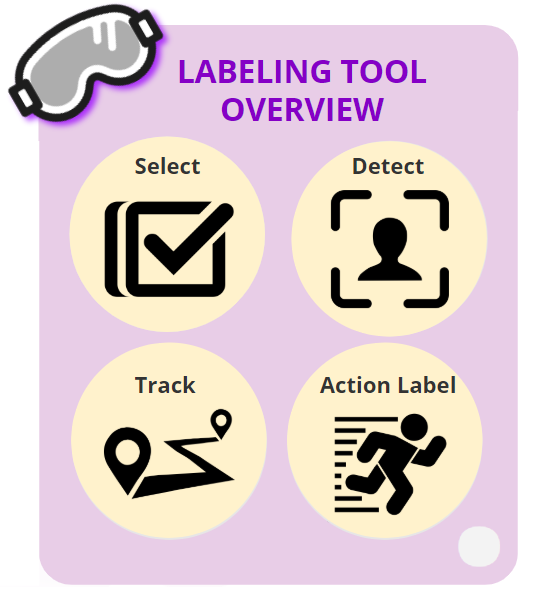
\includegraphics[width=0.5\textwidth]{chapter3/images/3_6/labelingToolOverview.png}
    \caption{กระบวนการหลักของเครื่องมือสำหรับกำกับข้อมูลด้วยปัญญาประดิษฐ์}
    \label{fig:labeling_overview}
\end{figure}
\clearpage

\subsection*{โดยแต่ละกระบวนการจะมีรายละเอียดดังนี้}
\subsubsection{Select}
กระบวนการ Select จะต้องสามารถรับวิดีโอเข้ามา แล้วตัดวิดีโอในช่วงที่ไม่มนุษย์อยู่ในเฟรมออกได้อัตโนมัติด้วยปัญญาประดิษฐ์
แต่เนื่องจากการประมวลผลทุกเฟรมในวิดีโอนั้นจะทำให้เสียเวลามากเกินไป จึงใช้วิธีการเลือกตัวอย่างเฟรมด้วยอัตราคงที่ (สามารถกำหนดได้)
ซึ่งเรียกว่าเฟรมเหล่านี้ว่า คีย์เฟรม จากนั้นใช้ปัญญาประดิษฐ์ประมวลผลคีย์เฟรมที่เหล่านั้น 
เพื่อลดระยะเวลาในการประมวลผลลง และมนุษย์จะต้องสามารถแก้ไขข้อผิดพลาดของปัญญาประดิษฐ์ได้ 
เพื่อเพิ่มคุณภาพของชุดข้อมูล จึงออกแบบหน้าต่างได้ดังรูปที่ \ref{fig:SelectDraft}

\begin{figure}[!ht]
    \centering
    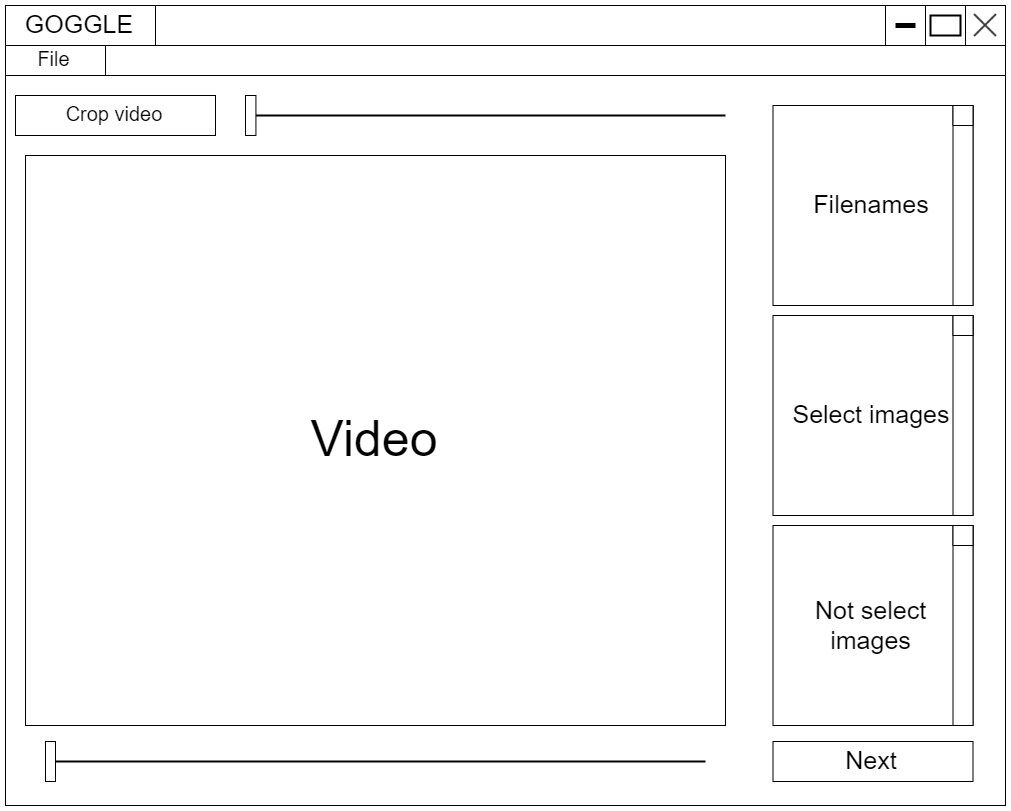
\includegraphics[width=1\textwidth]{chapter3/images/3_6/SelectDraft.png}
    \caption{หน้าต่าง Select ของเครื่องมือสำหรับกำกับข้อมูลด้วยปัญญาประดิษฐ์}
    \label{fig:SelectDraft}
\end{figure}
\clearpage
\begin{figure}[!ht]
    \centering
    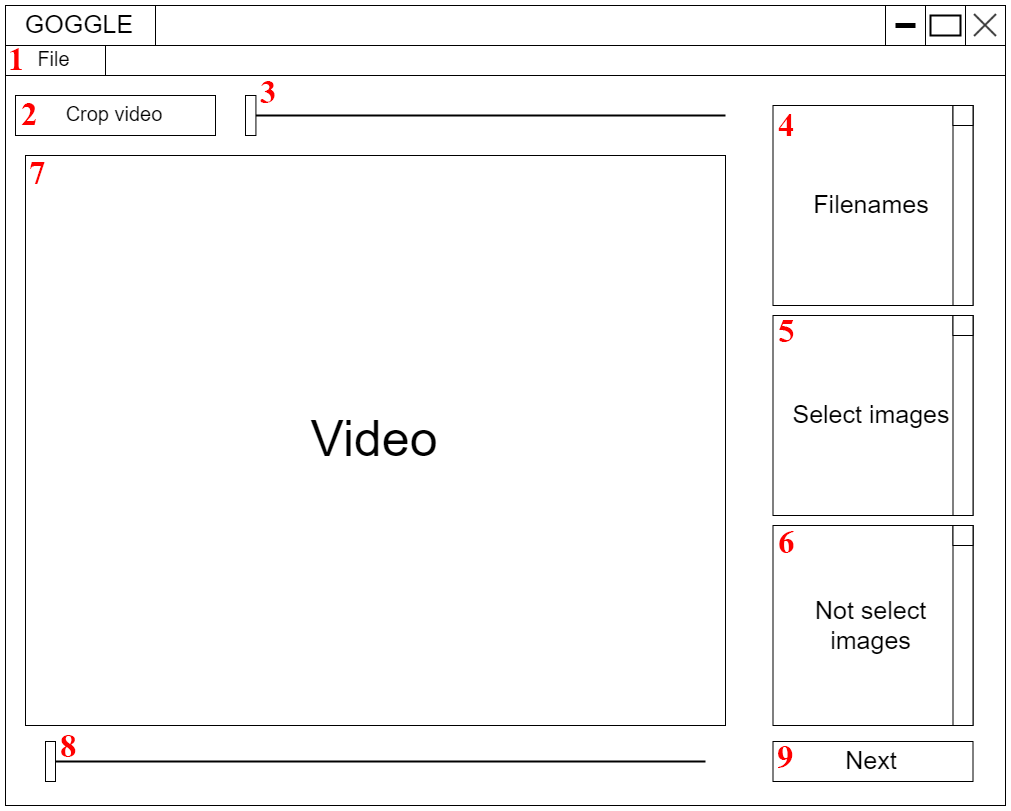
\includegraphics[width=1\textwidth]{chapter3/images/3_6/SelectDraft_point.png}
    \caption{ตำแหน่งของแต่ละวิดเจ็ตในหน้าต่าง Select}
    \label{fig:SelectDraft_point}
\end{figure}
โดยที่แต่ละวิดเจ็ตตามหมายเลขที่กำหนดตามรูปที่ \ref{fig:SelectDraft_point} มีรายละเอียดดังนี้
\begin{enumerate}
	\setlength\itemsep{-0.25em}
	\item หมายเลข 1 คือปุ่มสำหรับเลือกไฟล์วิดีโอที่ต้องการจากในคอมพิวเตอร์เข้ามาในโปรแกรม
    \item หมายเลข 2 คือปุ่มสำหรับสั่งให้ระบบทำการสร้างคีย์เฟรมขึ้นมา แล้วใช้ปัญญาประดิษฐ์ประมวลผลเพื่อแยกว่าคีย์เฟรมไหนมีคนอยู่ และคีย์เฟรมไหนไม่มีคนอยู่แบบอัตโนมัติ
    \item หมายเลข 3 คือแถบเลื่อนเพื่อกำหนดความถี่ในการหยิบคีย์เฟรม โดยจะมีช่วงอยู่ที่ 1 เฟรมต่อวินาที จนถึง อัตราเฟรมต่อวินาทีสูงสุดของวิดีโอที่รับเข้ามา
	\item หมายเลข 4 คือกล่องสำหรับแสดงชื่อวิดีโอที่รับเข้ามาในโปรแกรมเพื่อเลือกเข้ามาใช้ในการประมวลผล
	\item หมายเลข 5 คือกล่องสำหรับแสดงว่าคีย์เฟรมใดมีมนุษย์อยู่ในเฟรม โดยที่ผู้ใช้งานสามารถตรวจสอบความถูกต้องและแก้ไขข้อผิดพลาดของปัญญาประดิษฐ์ได้
	\item หมายเลข 6 คือกล่องสำหรับแสดงว่าคีย์เฟรมใดไม่มีมนุษย์อยู่ในเฟรม โดยที่ผู้ใช้งานสามารถตรวจสอบความถูกต้องและแก้ไขข้อผิดพลาดของปัญญาประดิษฐ์ได้
	\item หมายเลข 7 คือหน้าต่างสำหรับแสดงเฟรมที่เลือกจากหมายเลข 5 หมายเลข 6 หรือหมายเลข 8
	\item หมายเลข 8 คือแถบเลื่อนสำหรับเลื่อนดูคีย์เฟรมทั้งหมดที่ระบบสร้างขึ้น
	\item หมายเลข 9 คือปุ่มสำหรับไปกระบวนการต่อไปหลังจากระบบประมวลผลเสร็จแล้ว
\end{enumerate}
\clearpage

\subsubsection{Detect}
กระบวนการ Delect จะต้องสามารถรับคีย์เฟรมจากกระบวนการ Select มาประมวลผลด้วยปัญญาประดิษฐ์เพื่อหาตำแหน่งของมนุษย์ที่อยู่ในคีย์เฟรม 
แล้วสร้างกรอบสี่เหลี่ยมครอบบริเวณดังกล่าวได้ในแบบอัตโนมัติ เพื่อแบ่งเบาภาระผู้ใช้ในการที่ต้องสร้างกรอบสี่เหลี่ยมครอบตำแหน่งของมนุษย์ด้วยตัวเอง
และผู้ใช้ต้องสามารถสร้างหรือลบกรอบสี่เหลี่ยมได้ด้วยตัวเองสำหรับแก้ไขความผิดพลาดของปัญญาประดิษฐ์ เพื่อเพิ่มคุณภาพของชุดข้อมูล
จึงออกแบบหน้าต่างได้ดังรูปที่ \ref{fig:DetectDraft}
\begin{figure}[!ht]
    \centering
    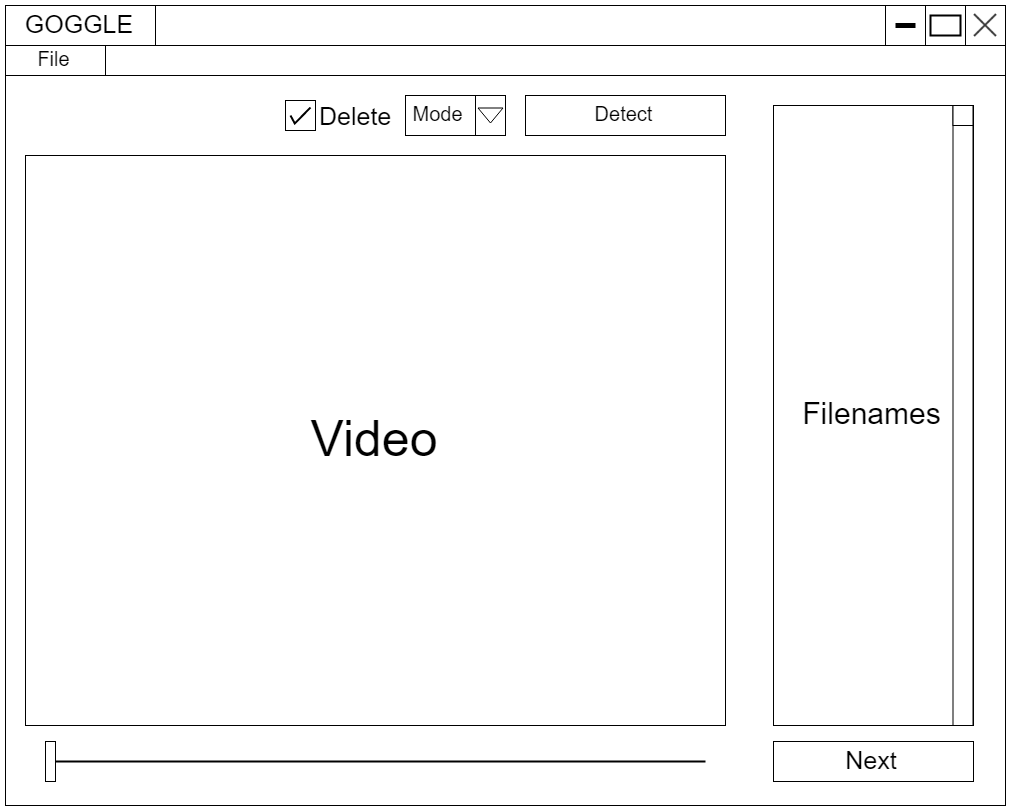
\includegraphics[width=1\textwidth]{chapter3/images/3_6/DetectDraft.png}
    \caption{หน้าต่าง Detect ของเครื่องมือสำหรับกำกับข้อมูลด้วยปัญญาประดิษฐ์}
    \label{fig:DetectDraft}
\end{figure}
\clearpage
\begin{figure}[!ht]
    \centering
    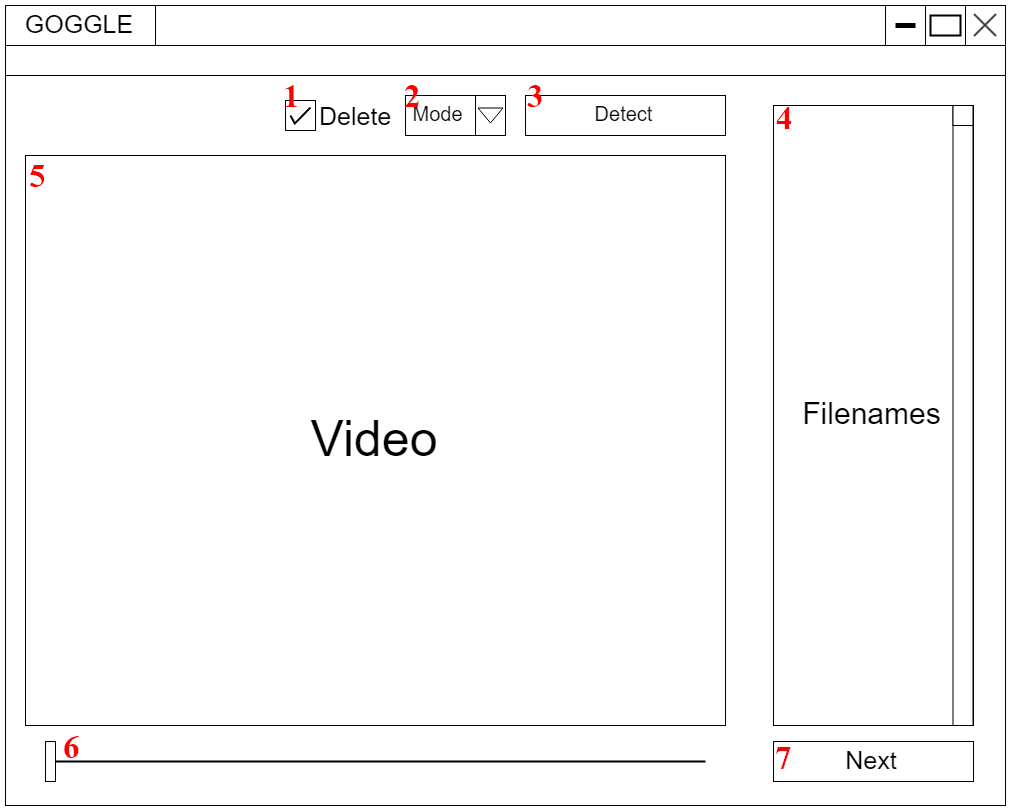
\includegraphics[width=1\textwidth]{chapter3/images/3_6/DetectDraft_point.png}
    \caption{ตำแหน่งของแต่ละวิดเจ็ตในหน้าต่าง Detect}
    \label{fig:DelectDraft_point}
\end{figure}
โดยที่แต่ละวิดเจ็ตตามหมายเลขที่กำหนดตามรูปที่ \ref{fig:DelectDraft_point} มีรายละเอียดดังนี้
\begin{enumerate}
	\setlength\itemsep{-0.25em}
    \item หมายเลข 1 คือช่องสำหรับกดเพื่อเปลี่ยนระบบจากสร้างกรอบสี่เหลี่ยมในแบบแก้ไขด้วยตนเองเป็นลบกรอบสี่เหลี่ยมแทน
    \item หมายเลข 2 คือช่องสำหรับเลือกว่าจะใช้ระบบแบบใด ระหว่างแบบอัตโนมัติและแบบแก้ไขด้วยตนเอง
    \item หมายเลข 3 คือปุ่มสำหรับสั่งให้ระบบทำการตรวจหาตำแหน่งของมนุษย์ในคีย์เฟรมทั้งหมดแล้วสร้างกรอบสี่เหลี่ยมขึ้นมาครอบบริเวณที่กำหนด
	\item หมายเลข 4 คือกล่องสำหรับแสดงคีย์เฟรมทั้งหมด
	\item หมายเลข 5 คือหน้าต่างสำหรับแสดงเฟรมที่เลือกจากหมายเลข 4 หรือหมายเลข 6
	\item หมายเลข 6 คือแถบเลื่อนสำหรับเลื่อนดูคีย์เฟรมทั้งหมดที่มี เพื่อตรวจสอบความถูกต้องของปัญญาประดิษฐ์
	\item หมายเลข 7 คือปุ่มสำหรับไปกระบวนการต่อไปหลังจากระบบประมวลผลเสร็จแล้ว
\end{enumerate}
\clearpage

\subsubsection{Track}
เนื่องจากกระบวนการ Detect นั้นจะทำเฉพาะในคีย์เฟรมทำให้ในเฟรมอื่นๆนอกเหนือจากนั้นจะไม่มีกรอบสี่เหลี่ยมอยู่
ดังนั้นกระบวนการ Track จึงต้องสามารถทำนายตำแหน่งต่อไปของมนุษย์แล้วสร้างกรอบสี่เหลี่ยมขึ้นมาบนเฟรมระหว่างคีย์เฟรมทั้งหมดได้โดยอัตโนมัติ
เพื่อสร้างข้อมูลตำแหน่งของมนุษย์ในเฟรมเหล่านั้น และผู้ใช้ต้องสามารถสร้างหรือลบกรอบสี่เหลี่ยมได้ด้วยตัวเองสำหรับแก้ไขความผิดพลาดของอัลกอริทึม
จึงออกแบบหน้าต่างได้ดังรูปที่ \ref{fig:TrackDraft}
\begin{figure}[!ht]
    \centering
    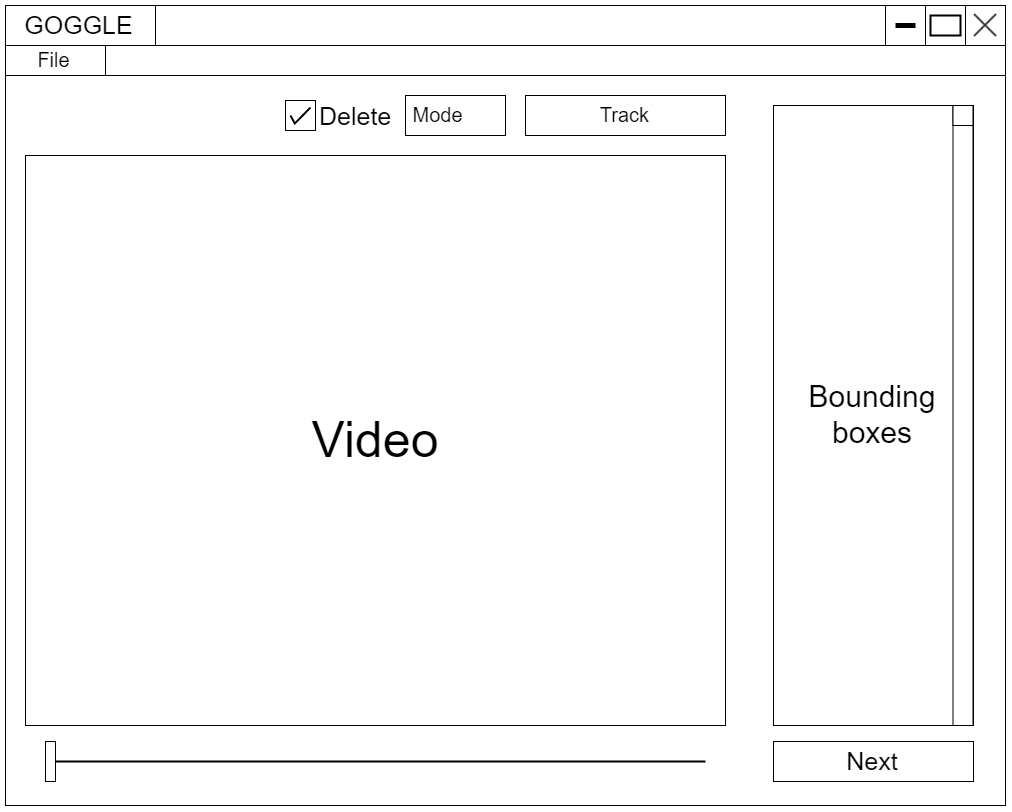
\includegraphics[width=1\textwidth]{chapter3/images/3_6/TrackDraft.png}
    \caption{หน้าต่าง Track ของเครื่องมือสำหรับกำกับข้อมูลด้วยปัญญาประดิษฐ์}
    \label{fig:TrackDraft}
\end{figure}
\clearpage
\begin{figure}[!ht]
    \centering
    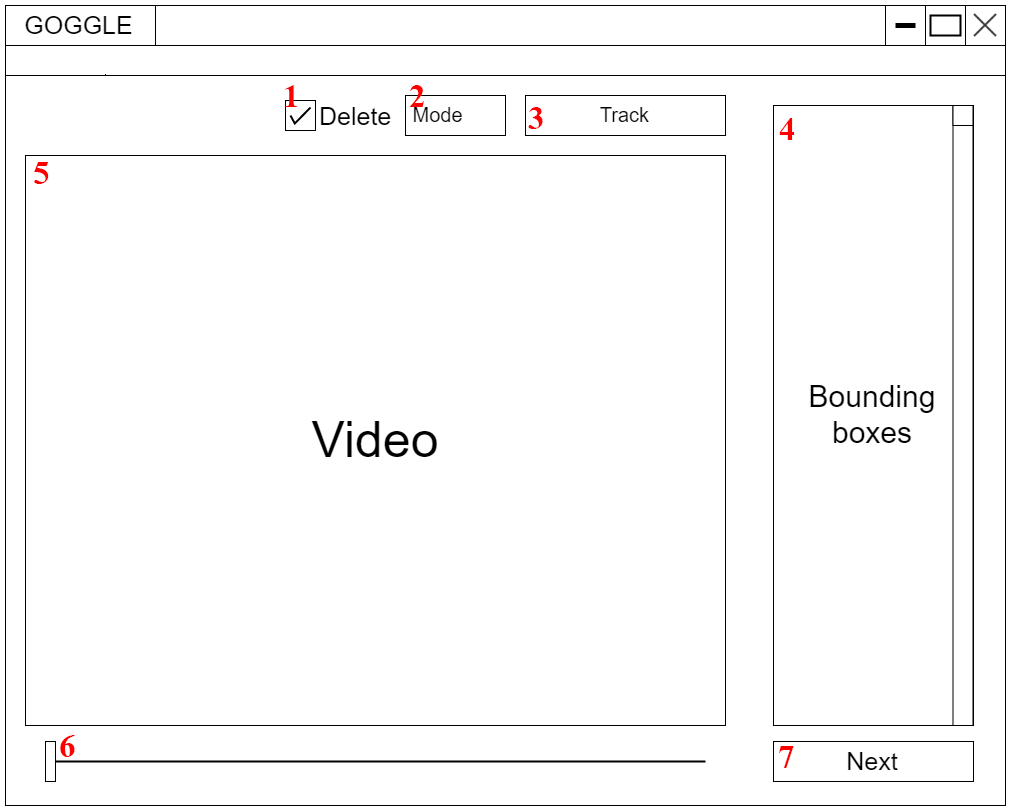
\includegraphics[width=1\textwidth]{chapter3/images/3_6/TrackDraft_point.png}
    \caption{ตำแหน่งของแต่ละวิดเจ็ตในหน้าต่าง Track}
    \label{fig:TrackDraft_point}
\end{figure}
โดยที่แต่ละวิดเจ็ตตามหมายเลขที่กำหนดตามรูปที่ \ref{fig:TrackDraft_point} มีรายละเอียดดังนี้
\begin{enumerate}
	\setlength\itemsep{-0.25em}
    \item หมายเลข 1 คือช่องสำหรับกดเพื่อเปลี่ยนระบบจากสร้างกรอบสี่เหลี่ยมในแบบแก้ไขด้วยตนเองเป็นลบกรอบสี่เหลี่ยมแทน
    \item หมายเลข 2 คือช่องสำหรับเลือกว่าจะใช้ระบบแบบใด ระหว่างแบบอัตโนมัติและแบบแก้ไขด้วยตนเอง
    \item หมายเลข 3 คือปุ่มสำหรับสั่งให้ระบบทำการตรวจหาตำแหน่งของมนุษย์ในเฟรมระหว่างคีย์เฟรมทั้งหมดแล้วสร้างกรอบสี่เหลี่ยมขึ้นมาครอบบริเวณที่กำหนด
	\item หมายเลข 4 คือกล่องสำหรับแสดงกรอบสี่เหลี่ยมทั้งหมดที่อยู่ในเฟรม
	\item หมายเลข 5 คือหน้าต่างสำหรับแสดงเฟรมที่เลือกจากหมายเลข 6
	\item หมายเลข 6 คือแถบเลื่อนสำหรับเลื่อนดูเฟรมทั้งหมดที่มี เพื่อตรวจสอบความถูกต้องของอัลกอริทึม
	\item หมายเลข 7 คือปุ่มสำหรับไปกระบวนการต่อไปหลังจากระบบประมวลผลเสร็จแล้ว
\end{enumerate}
\clearpage

\subsubsection{Label}
กระบวนการ Label นั้นต้องสามารถทำนายว่าการกระทำของมนุษย์ที่อยู่ในแต่ละเฟรมว่าคืออะไรได้โดยอัตโนมัติด้วยปัญญาประดิษฐ์
และผู้ใช้จะต้องสามารถแก้ไขข้อผิดพลาดของปัญญาประดิษฐ์ได้หากมีการทำนายที่ผิดพลาดเกิดขึ้น
หรือถ้าหากผู้ใช้ต้องการเพิ่มการกระทำที่ไม่ได้มีอยู่ในชุดการกระทำพื้นฐานที่มีอยู่แล้วของปัญญาประดิษฐ์ ผู้ใช้ก็สามารถเพิ่มการกระทำนั้นเข้ามาได้
จึงออกแบบหน้าต่างได้ดังรูปที่ \ref{fig:ActionLabelDraft}
\begin{figure}[!ht]
    \centering
    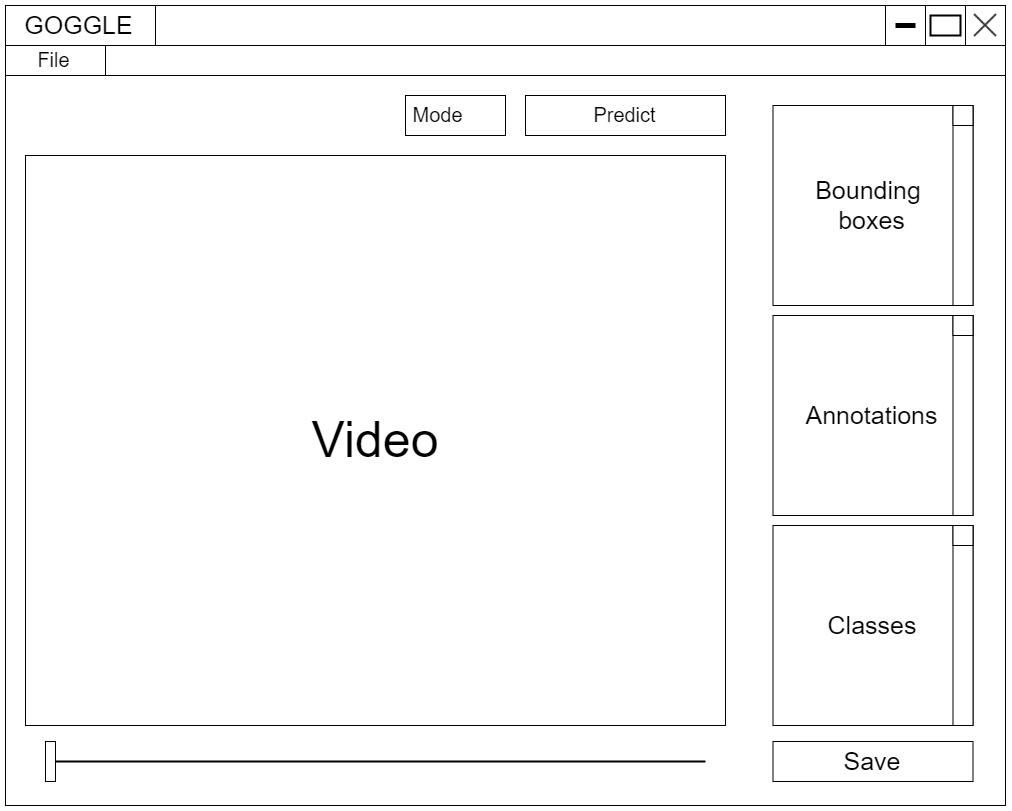
\includegraphics[width=1\textwidth]{chapter3/images/3_6/ActionLabelDraft.png}
    \caption{หน้าต่าง Label ของเครื่องมือสำหรับกำกับข้อมูลด้วยปัญญาประดิษฐ์}
    \label{fig:ActionLabelDraft}
\end{figure}
\clearpage
\begin{figure}[!ht]
    \centering
    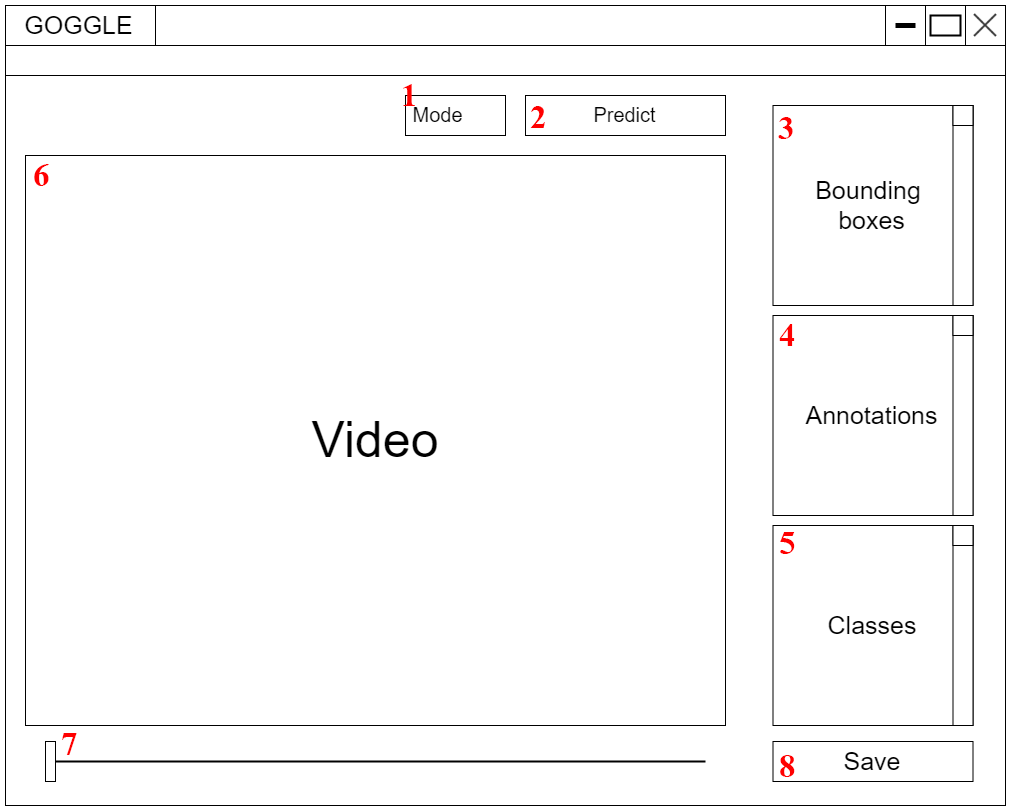
\includegraphics[width=1\textwidth]{chapter3/images/3_6/ActionLabelDraft_point.png}
    \caption{ตำแหน่งของแต่ละวิดเจ็ตในหน้าต่าง Label}
    \label{fig:ActiobLabelDraft_point}
\end{figure}
โดยที่แต่ละวิดเจ็ตตามหมายเลขที่กำหนดตามรูปที่ \ref{fig:TrackDraft_point} มีรายละเอียดดังนี้
\begin{enumerate}
	\setlength\itemsep{-0.25em}
    \item หมายเลข 1 คือช่องสำหรับเลือกว่าจะใช้ระบบแบบใด ระหว่างแบบอัตโนมัติและแบบแก้ไขด้วยตนเอง
    \item หมายเลข 2 คือปุ่มสำหรับสั่งให้ระบบทำนายการกระทำของมนุษย์ในทุกๆเฟรม
    \item หมายเลข 3 คือกล่องสำหรับแสดงกรอบสี่เหลี่ยมทั้งหมดที่อยู่ในเฟรมที่เลือก
	\item หมายเลข 4 คือกล่องสำหรับแสดงการกระทำของมนุษย์แต่ละคนที่อยู่ในเฟรมที่เลือก โดยจะเรียงลำดับคู่กับกรอบสี่เหลี่ยมที่อยู่ในช่องหมายเลข 3
    \item หมายเลข 5 คือกล่องสำหรับแสดงชุดการกระทำที่ปัญญาประดิษฐ์มีอยู่แล้ว ซึ่งในการทำงานแบบแก้ไขด้วยตนเองนั้น จะสามารถค้นหาการกระทำที่มีอยู่แล้วได้ 
    และหากคำที่ใส่เข้ามานั้นไม่มีอยู่ในชุดการกระทำก็จะเป็นการเพิ่มการกระทำนั้นเข้ามาแทน
	\item หมายเลข 6 คือหน้าต่างสำหรับแสดงเฟรมที่เลือกจากหมายเลข 7
	\item หมายเลข 7 คือแถบเลื่อนสำหรับเลื่อนดูเฟรมทั้งหมดที่มี เพื่อตรวจสอบความถูกต้องของปัญญาประดิษฐ์
	\item หมายเลข 8 คือปุ่มสำหรับสร้างไฟล์ xml ของทุกๆเฟรมสำหรับใช้ในการสร้างโมเดลโดยรายละเอียดข้อมูลภายในไฟล์ xml จะอยู่ในหัวข้อ \ref{sec:XMLInfo}
\end{enumerate}
\clearpage

\subsubsection{รายละเอียดข้อมูลภายในไฟล์ xml}
\label{sec:XMLInfo}
ไฟล์ xml นั้นเป็นรูปแบบที่นิยมใช้ในการเก็บข้อมูลสำหรับการสร้างโมเดลประเภทตรวจจับวัตถุ
โดยจะเก็บข้อมูลในรูปแบบของ PASCAL VOC ที่นิยมใช้ในการสร้างโมเดลด้วย Tensorflow โดยภายในไฟล์จะมีข้อมูลดังรูปที่ \ref{fig:XMLFormat}
\begin{figure}[!ht]
    \centering
    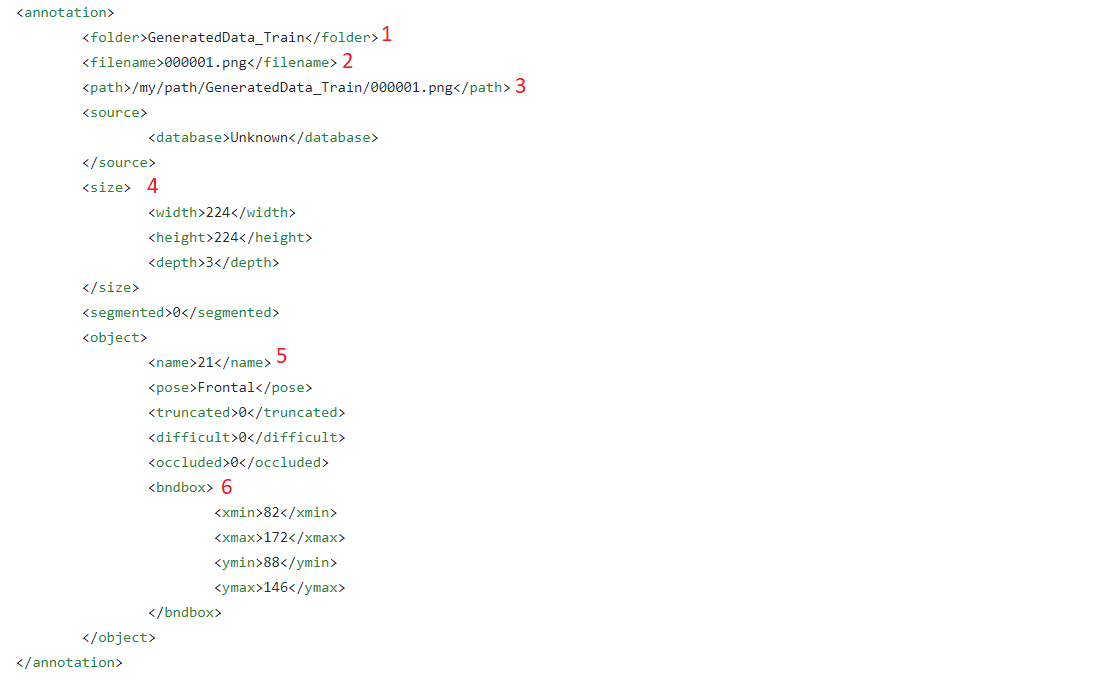
\includegraphics[width=1\textwidth]{chapter3/images/3_6/XMLFormat.png}
    \caption{ตัวอย่างข้อมูลภายในไฟล์ xml}
    \label{fig:XMLFormat}
\end{figure}
โดยข้อมูลส่วนสำคัญของรูปแบบนี้นั้นจะถูกใส่หมายเลขกำกับไว้ซึ่งแต่ละหมายเลขนั้นหมายถึง
\begin{enumerate}
	\setlength\itemsep{-0.25em}
    \item หมายเลข 1 คือชื่อโฟลเดอร์ที่เก็บไฟล์รูปภาพที่เกี่ยวข้องกับไฟล์ xml นี้อยู่
    \item หมายเลข 2 คือชื่อไฟล์ที่เกี่ยวข้องกับไฟล์ xml นี้
    \item หมายเลข 3 คือเส้นทางในคอมพิวเตอร์ (directory path) ของไฟล์รูปภาพที่เกี่ยวข้องกับไฟล์ xml นี้
    \item หมายเลข 4 คือขนาดและมิติของรูปภาพ ซึ่งจะประกอบด้วยความกว้าง (width) ความยาว (height) และจำนวนช่องสี (depth) 
    โดยที่จำนวนช่องสีที่มีความลึก 3 มักจะหมายถึงภาพสี RGB และจำนวนช่องสีที่มีความลึก 2 จะหมายถึงภาพขาวดำ (gray scale)
	\item หมายเลข 5 คือ label ของวัตถุหรืออย่างอื่น ที่อยู่ในกรอบสี่เหลี่ยมที่ถูกกำหนดไว้ในส่วนของหมายเลข 6
	\item หมายเลข 6 คือ กรอบสี่เหลี่ยมที่ครอบวัตถุที่สนใจ เช่นมนุษย์ เป็นต้น
\end{enumerate}
\clearpage

\section{การออกแบบการทดสอบการตรวจจับวัตถุ}
\subsection{ทดสอบประสิทธิ์ภาพการทำงานของโมเดลปัญญาประดิษฐ์สำหรับการทำการตรวจจับภาพบุคคล}
\subsection*{สิ่งที่ใช้ในการวัดผล}
	\begin{enumerate}
		\setlength\itemsep{-0.25em}
		\item ความเร็วในการทำนายต่อรูปภาพ (มิลลิวินาที)
		\item ความแม่นยำ โดยคำนึงถึงอัตราส่วนร่วมของกรอบที่เหลี่ยม หรือ Intersection over Union (IoU)
	\end{enumerate}
\subsection*{จุดประสงค์}
	\begin{enumerate}
		\setlength\itemsep{-0.25em}
		\item ผู้วิจัยได้ตั้งจุดประสงค์การทดลองการใช้โมเดลปัญญาประดิษฐ์สำหรับตรวจจับวัตถุ เพื่อวัดผลโมเดลปัญญาประดิษฐ์ที่ใช้ในปัจจุบัน
และหาโมเดลปัญญาประดิษฐ์สำหรับการตรวจจับวัตถุที่มีความเร็วมากที่สุดและแม่นยำสูงที่สุดเมื่อทดสอบกับชุดข้อมูลของผู้วิจัย
	\end{enumerate}
\subsection*{ตัวแปร}
	\begin{enumerate}
		\setlength\itemsep{-0.25em}
		\item โมเดลปัญญาประดิษฐ์ ได้แก่
		\begin{enumerate}
			\setlength\itemsep{-0.25em}
			\item SSD Mobilenet v1 ppn
			\item YOLO-v3 tiny
			\item YOLO-v3 spp	
			\item YOLO-v3 320
			\item Faster RCNN inception v2
		\end{enumerate}
	\end{enumerate}
\subsection*{ตัวแปรควบคุม}
	\begin{enumerate}
		\setlength\itemsep{-0.25em}
		\item ชุดข้อมูล : ชุดข้อมูลสำหรับทดสอบวัดผลที่ผู้วิจัยสร้างขึ้น (สุ่ม 20 เฟรมจากวิดีโอที่ผู้วิจัยใช้สำหรับสร้างชุดข้อมูล)
	\end{enumerate}
\subsection*{วิธีการทดลอง}
	\begin{enumerate}
		\setlength\itemsep{-0.25em}
		\item แบ่งชุดข้อมูลออกเป็นชุดข้อมูลสำหรับทดสอบ และชุดข้อมูลที่มีคำกำกับเพื่อเป็นคำตอบ
			\begin{enumerate}
				\setlength\itemsep{-0.25em}
				\item ชุดข้อมูลสำหรับทดสอบ ประกอบด้วย : ชื่อของวิดีโอ และเฟรม
				\item ชุดข้อมูลที่มีคำกำกับเพื่อเป็นคำตอบ ประกอบด้วย : ชื่อของวิดีโอ เฟรม และตำแหน่งของกรอบสี่เหลี่ยม
			\end{enumerate}
		\item เรียกชื่อและเฟรมของวิดีโอจากชุดข้อมูลทดสอบ และนำโมเดลปัญญาประดิษฐ์ทำนายผลลัพธ์ จากนั้นเก็บผลลัพธ์เป็นชุดข้อมูลผลลัพธ์จากการทำนาย
			\begin{enumerate}
				\setlength\itemsep{-0.25em}
				\item ชุดข้อมูลผลลัพธ์จากการทำนาย ประกอบด้วย : ชื่อของวิดีโอ เฟรม และตำแหน่งของกรอบสี่เหลี่ยม
			\end{enumerate}
		\item ประเมินผลค่าความแม่นยำในการทำงานโดยเทียบระหว่างชุดผลลัพธ์จากการทำนาย และชุดข้อมูลที่มีคำกำกับเพื่อเป็นคำตอบ โดยกำหนดให้ค่า IoU >= 0.5	จึงจะนับว่าทำนายได้ถูก
		\item เปรียบเทียบผลลัพธ์จากแหล่งที่มา
\end{enumerate}

\clearpage

\section{การออกแบบการทดสอบการทำนายตำแหน่งต่อไปของมนุษย์}
\subsection{ทดสอบประสิทธิ์ภาพการทำงานของระบบทำนายตำแหน่งต่อไปของวัตถุในวิดีโอ}
\subsection*{สิ่งที่ใช้ในการวัดผล}
	\begin{enumerate}
		\item ความเร็วในการทำนายต่อวิดีโอ (วินาที)
		\item ความแม่นยำ โดยคำนึงถึงอัตราส่วนร่วมของกรอบที่เหลี่ยม
	\end{enumerate}
\subsection*{สมมุติฐาน}
ผู้วิจัยได้ตั้งสมมุติฐานว่า การใช้โมเดลปัญญาประดิษฐ์สำหรับตรวจจับวัตถุและสร้างกรอบสี่เหลี่ยมทุกๆ N เฟรม 
แล้วใช้ระบบทำนายตำแหน่งต่อไปของวัตถุในการสร้างกรอบสี่เหลี่ยมในเฟรมระหว่างนั้น จะทำให้ระบบสามารถทำงานได้เร็วขึ้น โดยที่ประสิทธิภาพจะลดลงเพียงเล็กน้อย
\subsection*{ตัวแปรควบคุม}
	\begin{enumerate}
		\item วิดีโอสาธารณะที่ไม่ติดลิขสิทธิ์ ความยาวประมาณ 10 - 30 วินาที หนึ่งวิดีโอ
		\item ใช้โมเดลปัญญาประดิษฐ์สำหรับตรวจจับตำแหน่งวัตถุ ResNet50 ในการสร้างชุดข้อมูลที่มีการกำกับตำแหน่งวัตถุไว้ (ground-truth) แล้วใช้มนุษย์ในการตรวจสอบความถูกต้อง
		เพื่อใช้เป็นคำตอบของการทำนาย
		\item โมเดลปัญญาประดิษฐ์สำหรับตรวจจับตำแหน่งที่ใช้ในการเปรียบเทียบ: YOLO-V3 320
		\item อัลกอริทึมสำหรับระบบทำนายตำแหน่งต่อไปของวัตถุ: dlib
		\item อัตราส่วนร่วมของกรอบที่เหลี่ยม: มีส่วนที่ทับกันมากกว่า 80\% ขึ้นไปจึงจะนับว่าผลการทำนายถูกต้อง
	\end{enumerate}
\subsection*{วิธีการทดลอง}
	\begin{enumerate}
		\item ใช้โมเดลปัญญาประดิษฐ์ YOLO-v3 320 ประมวลผลทุกเฟรมในวิดีโอ และเปรียบเทียบผลลัพธ์กับชุดข้อมูลที่ถูกกำกับตำแหน่งวัตถุไว้แล้ว เพื่อคำนวณหาความแม่นยำ
		\item ใช้โมเดลปัญญาประดิษฐ์ YOLO-v3 320 ประมวลผลทุกๆ N เฟรมในวิดีโอ แล้วใช้ระบบทำนายตำแหน่งต่อไปของวัตถุในการสร้างกรอบสี่เหลี่ยมในเฟรมระหว่างนั้น 
		และเปรียบเทียบผลลัพธ์กับชุดข้อมูลที่ถูกกำกับตำแหน่งวัตถุไว้แล้ว เพื่อคำนวณหาความแม่นยำ โดยที่ค่า N จะเท่ากับ 10 20 และ 25
		\item เปรียบเทียบความเร็วในการประมวลผล และความแม่นยำ
\end{enumerate}
\clearpage

\section{การออกแบบการทดสอบการระบุตัวตนของมนุษย์}
\subsection{ทดสอบประสิทธิ์ภาพการทำงานของระบบระบุตัวตนของบุคคลภายในภาพ}
\subsection*{สิ่งที่ใช้ในการวัดผล}
	\begin{enumerate}
		\setlength\itemsep{-0.25em}
		\item ค่า AUC ที่ใช้สำหรับการระบุตัวตนของบุคคลภายในภาพ
	\end{enumerate}
\subsection*{สมมติฐาน}
ผู้วิจัยได้ตั้งสมมติฐานว่า ผลลัพธ์ของการทดลองการใช้งานจริงของโมเดลปัญญาประดิษฐ์ ResNet50 ที่สร้างด้วยชุดข้อมูล Market1501 
นั้นควรจะมีความแม่นยำในการระบุตัวตนของบุคคลภายในภาพมากที่สุดเมื่อเทียบกับโมเดลปัญญาประดิษฐ์ที่สร้างด้วยชุดข้อมูลอื่นๆ
เพราะเมื่อเทียบกับโมเดลปัญญาประดิษฐ์ที่ถูกสร้างด้วยชุดข้อมูลอื่นที่มาจากแหล่งข้อมูลเดียวกัน โมเดลปัญญาประดิษฐ์ ResNet50 ที่สร้างด้วยชุดข้อมูล Market1501 นั้นจะมีความแม่นยำสูงสุด
\subsection*{ตัวแปร}
	\begin{enumerate}
		\setlength\itemsep{-0.25em}
		\item โมเดลปัญญาประดิษฐ์ ซึ่งได้แก่
		\begin{enumerate}
			\setlength\itemsep{-0.25em}
			\item ResNet50 ที่ถูกสร้างด้วยชุดข้อมูล Market1501
			\item ResNet50 ที่ถูกสร้างด้วยชุดข้อมูล DukeMTMCReID
			\item ResNet50 ที่ถูกสร้างด้วยชุดข้อมูล CUHK03	
			\item ResNet50 ที่ถูกสร้างด้วยชุดข้อมูล MSMT17
		\end{enumerate}
	\end{enumerate}
\subsection*{ตัวแปรควบคุม}
	\begin{enumerate}
		\setlength\itemsep{-0.25em}
		\item ชุดข้อมูล : ชุดข้อมูลที่ทางผู้วิจัยสร้างขึ้นสำหรับการทดสอบ
		\item โมเดลปัญญาประดิษฐ์ : YOLO-V3 320  สำหรับการหาตำแหน่งของบุคคล
	\end{enumerate}
\subsection*{วิธีการทดลอง}
	\begin{enumerate}
		\setlength\itemsep{-0.25em}
		\item นำชุดข้อมูลที่ผู้วิจัยสร้างขึ้นมาผ่านโมเดลปัญญาประดิษฐ์ YOLO-V3 320 เพื่อหาตำแหน่งของบุคคล
		\item นำโมเดลปัญญาประดิษฐ์แต่ละอันมาทดสอบความแม่นยำสำหรับการระบุตัวตนของบุคคลภายในภาพ ด้วยตำแหน่งของบุคคลที่ได้มาจากขั้นตอนก่อนหน้านี้
		\item ประเมินผลการทำงานโดยเทียบค่า AUC สำหรับการระบุตัวตนของบุคคลภายในภาพของแต่ละโมเดลปัญญาประดิษฐ์ เพื่อหาโมเดลปัญญาประดิษฐ์ที่เหมาะสมกับชุดข้อมูลของผู้วิจัยมากที่สุด
\end{enumerate}

\clearpage

\section{การออกแบบการทดสอบการจดจำการกระทำของมนุษย์}
\subsection{ทดสอบประสิทธิ์ภาพการทำงานของโมเดลปัญญาประดิษฐ์ที่เคยถูกเทรนด์ผ่าน AVA โดยใช้ชุดข้อมูลของ AVA ในการทดสอบและเทียบผลลัพธ์กับแหล่งอ้างอิง}
\subsection*{สิ่งที่ใช้ในการวัดผล}
	\begin{enumerate}
		\setlength\itemsep{-0.25em}
		\item ความเร็วในการทำนายต่อรูปภาพ (มิลลิวินาที)
		\item ความแม่นยำ (PASCAL mAP)
	\end{enumerate}
\subsection*{สมมุติฐาน}
ผู้วิจัยได้ตั้งสมมุติฐานว่า ผลลัพธ์ของการทดลองจะมีความแม่นยำเทียบเท่ากับผลลัพธ์จากแหล่งที่มา แต่ความเร็วต่อรูปภาพจะมีความเร็วน้อยกว่าผลลัพธ์จากแหล่งที่มา 
เนื่องจากแหล่งที่มาของข้อมูลได้ทำการทดสอบโดยใช้กราฟิกการ์ดรุ่น Nvidia GeForce GTX TITAN X ซึ่งเป็นกราฟิกการ์ดที่มีประสิทธิภาพการทำงานดีกว่ากราฟิกการ์ดของผู้วิจัย จึงทำให้สามารถทดสอบด้วยความเร็วที่มากกว่า
\subsection*{ตัวแปรควบคุม}
	\begin{enumerate}
		\setlength\itemsep{-0.25em}
		\item ชุดข้อมูล : The validation split of AVA v2.1
		\item โมเดลปัญญาประดิษฐ์ : Faster RCNN ResNet101 AVA v2.1
	\end{enumerate}
\subsection*{วิธีการทดลอง}
	\begin{enumerate}
		\setlength\itemsep{-0.25em}
		\item ดาวน์โหลดชุดข้อมูล The validation split of AVA v2.1
		\item แบ่งชุดข้อมูลออกเป็น ชุดข้อมูลสำหรับทดสอบ และชุดข้อมูลที่มีคำกำกับเพื่อเป็นคำตอบ
			\begin{enumerate}
				\setlength\itemsep{-0.25em}
				\item ชุดข้อมูลสำหรับทดสอบ ประกอบด้วย : ชื่อของวิดีโอ
				\item ชุดข้อมูลที่มีคำกำกับเพื่อเป็นคำตอบ ประกอบด้วย : ชื่อของวิดีโอ เฟรม ตำแหน่งของกรอบสี่เหลี่ยม และรหัสของการกระทำ
			\end{enumerate}
		\item เรียกชื่อของวิดีโอจากชุดข้อมูลทดสอบ และนำโมเดลปัญญาประดิษฐ์ทำนายผลลัพธ์ จากนั้นเก็บผลลัพธ์เป็นชุดข้อมูลผลลัพธ์จากการทำนาย
			\begin{enumerate}
				\setlength\itemsep{-0.25em}
				\item ชุดข้อมูลผลลัพธ์จากการทำนาย ประกอบด้วย : ชื่อของวิดีโอ เฟรม ตำแหน่งของกรอบสี่เหลี่ยม รหัสของการกระทำ และความมั่นใจ
			\end{enumerate}
		\item ประเมินผลการทำงานโดยเทียบระหว่างชุดผลลัพธ์จากการทำนาย และชุดข้อมูลที่มีคำกำกับเพื่อเป็นคำตอบ
		\item เปรียบเทียบผลลัพธ์จากแหล่งที่มา
\end{enumerate}
\clearpage
\subsection{ทดสอบประสิทธิภาพการทำงานของโมเดลปัญญาประดิษฐ์ที่เคยถูกสร้างด้วย AVA และใช้ชุดข้อมูลที่ผู้วิจัยสร้างขึ้นในการทดสอบและเทียบผลลัพธ์กับแหล่งอ้างอิง}
\subsection*{สิ่งที่ใช้ในการวัดผล}
	\begin{enumerate}
		\setlength\itemsep{-0.25em}
		\item ความในการทำนายเร็วต่อรูปภาพ (มิลลิวินาที)
		\item ความแม่นยำ (PASCAL mAP)
	\end{enumerate}
\subsection*{สมมุติฐาน}ผู้วิจัยได้ตั้งสมมุติฐานว่าผลลัพธ์ของการทดลองจะมีความแม่นยำต่ำลงเมื่อเทียบกับความแม่นยำของการทดลองที่ผ่านมา เนื่องจากชุดข้อมูลที่ผู้วิจัยสร้างขึ้น ได้มีการตัดหมวดหมู่บางอย่างออกไป 
ทำให้โมเดลปัญญาประดิษฐ์ที่ถูกสร้างด้วย AVA มีหมวดหมู่ของการกระทำไม่ตรงกับชุดข้อมูลที่ผู้วิจัยสร้างขึ้น ซึ่งมีผลทำให้ความแม่นยำลดลง ในส่วนของความเร็วต่อรูปภาพจะมีความเร็วน้อยกว่าผลลัพธ์จากแหล่งที่มา เนื่องจาก แหล่งที่มาของข้อมูลได้ทำการทดสอบโดยใช้กราฟิกการ์ดรุ่น Nvidia GeForce GTX TITAN X card ซึ่งเป็นกราฟิกการ์ดที่มีประสิทธิภาพการทำงานดีกว่า กราฟิกการ์ดของผู้วิจัย จึงทำให้สามารถทดสอบด้วยความเร็วที่มากกว่า
\subsection*{ตัวแปรควบคุม}
	\begin{enumerate}
		\setlength\itemsep{-0.25em}
		\item ชุดข้อมูล : ชุดข้อมูลที่ผู้วิจัยสร้างด้วยเครื่องมือกำกับคุณลักษณะ
		\item โมเดลปัญญาประดิษฐ์ : Faster RCNN ResNet101 AVA v2.1
	\end{enumerate}
\subsection*{วิธีการทดลอง}
	\begin{enumerate}
		\setlength\itemsep{-0.25em}
		\item แบ่งชุดข้อมูลออกเป็น ชุดข้อมูลสำหรับทดสอบ และชุดข้อมูลที่มีคำกำกับเพื่อเป็นคำตอบ
			\begin{enumerate}
				\setlength\itemsep{-0.25em}
				\item ชุดข้อมูลสำหรับทดสอบ ประกอบด้วย : ชื่อของวิดีโอ
				\item ชุดข้อมูลที่มีคำกำกับเพื่อเป็นคำตอบ ประกอบด้วย : ชื่อของวิดีโอ เฟรม ตำแหน่งของกรอบสี่เหลี่ยม และรหัสของการกระทำ
			\end{enumerate}
		\item เรียกชื่อของวิดีโอจากชุดข้อมูลทดสอบ และนำโมเดลปัญญาประดิษฐ์ทำนายผลลัพธ์ จากนั้นเก็บผลลัพธ์เป็นชุดข้อมูลผลลัพธ์จากการทำนาย
			\begin{enumerate}
				\setlength\itemsep{-0.25em}
				\item ชุดข้อมูลผลลัพธ์จากการทำนาย ประกอบด้วย : ชื่อของวิดีโอ เฟรม ตำแหน่งของกรอบสี่เหลี่ยม รหัสของการกระทำ และความมั่นใจ
			\end{enumerate}
		\item ประเมินผลการทำงานโดยเทียบระหว่างชุดผลลัพธ์จากการทำนาย และชุดข้อมูลที่มีคำกำกับเพื่อเป็นคำตอบ	
		\item เปรียบเทียบผลลัพธ์กับผลการทดลองที่ผ่านมา
\end{enumerate}
\clearpage
\subsection{ทดสอบประสิทธิภาพการทำงานของโมเดลปัญญาประดิษฐ์ที่ถูกสร้างด้วยชุดข้อมูลที่ผู้วิจัยสร้างขึ้น และใช้ชุดข้อมูลที่ผู้วิจัยสร้างขึ้นในการทดสอบและเทียบผลลัพธ์กับแหล่งอ้างอิง}
\subsection*{สิ่งที่ใช้ในการวัดผล}
	\begin{enumerate}
		\setlength\itemsep{-0.25em}
		\item ความเร็วในการทำนายต่อรูปภาพ (มิลลิวินาที)
		\item ความแม่นยำ (PASCAL mAP)
	\end{enumerate}
\subsection*{สมมุติฐาน}ผู้วิจัยได้ตั้งสมมุติฐานว่าผลลัพธ์ของการทดลองจะมีความแม่นยำสูงขึ้นเมื่อเทียบกับความแม่นยำของการทดลองที่ผ่านมา เนื่องจากโมเดลปัญญาประดิษฐ์ในการทดลองนี้ 
เป็นโมเดลปัญญาประดิษฐ์ที่ผู้วิจัยได้สร้างขึ้น ซึ่งจะมีหมวดหมู่ของการกระทำของโมเดลปัญญาประดิษฐ์และชุดข้อมูลทดสอบตรงกัน ในส่วนของความเร็วต่อรูปภาพจะมีความเร็วน้อยกว่าผลลัพธ์จากแหล่งที่มา 
เนื่องจากแหล่งที่มาของข้อมูลได้ทำการทดสอบโดยใช้กราฟิกการ์ดรุ่น Nvidia GeForce GTX TITAN X ซึ่งเป็นกราฟิกการ์ดที่มีประสิทธิภาพการทำงานดีกว่ากราฟิกการ์ดของผู้วิจัย จึงทำให้สามารถทดสอบด้วยความเร็วที่มากกว่า
\subsection*{ตัวแปรควบคุม}
	\begin{enumerate}
		\setlength\itemsep{-0.25em}
		\item ชุดข้อมูล : ชุดข้อมูลที่ผู้วิจัยสร้างด้วยเครื่องมือกำกับคุณลักษณะ
		\item โมเดลปัญญาประดิษฐ์ : โมเดลปัญญาประดิษฐ์ที่ผู้วิจัยสร้างขึ้น
	\end{enumerate}
\subsection*{วิธีการทดลอง}
	\begin{enumerate}
		\setlength\itemsep{-0.25em}
		\item แบ่งชุดข้อมูลออกเป็น ชุดข้อมูลสำหรับทดสอบ และชุดข้อมูลที่มีคำกำกับเพื่อเป็นคำตอบ
			\begin{enumerate}
				\setlength\itemsep{-0.25em}
				\item ชุดข้อมูลสำหรับทดสอบ ประกอบด้วย : ชื่อของวิดีโอ
				\item ชุดข้อมูลที่มีคำกำกับเพื่อเป็นคำตอบ ประกอบด้วย : ชื่อของวิดีโอ เฟรม ตำแหน่งของกรอบสี่เหลี่ยม และรหัสของการกระทำ
			\end{enumerate}
		\item เรียกชื่อของวิดีโอจากชุดข้อมูลทดสอบ และนำโมเดลปัญญาประดิษฐ์ทำนายผลลัพธ์ จากนั้นเก็บผลลัพธ์เป็นชุดข้อมูลผลลัพธ์จากการทำนาย
			\begin{enumerate}
				\setlength\itemsep{-0.25em}
				\item ชุดข้อมูลผลลัพธ์จากการทำนาย ประกอบด้วย : ชื่อของวิดีโอ เฟรม ตำแหน่งของกรอบสี่เหลี่ยม รหัสของการกระทำ และความมั่นใจ
			\end{enumerate}
		\item ประเมินผลการทำงานโดยเทียบระหว่างชุดผลลัพธ์จากการทำนาย และ ชุดข้อมูลที่มีคำกำกับเพื่อเป็นคำตอบ	
		\item เปรียบเทียบผลลัพธ์กับผลการทดลองที่ผ่านมา
\end{enumerate}






	% ************************** Thesis Chapter4 **********************************
\chapter{ผลการดำเนินงาน}
\section{เครื่องมือกำกับคุณลักษณะ}
\subsection{หน้าต่างแสดงผลของแอพพลิเคชั่น}
\subsection*{หน้าต่าง Select}
\begin{figure}[!ht]
  \centering
    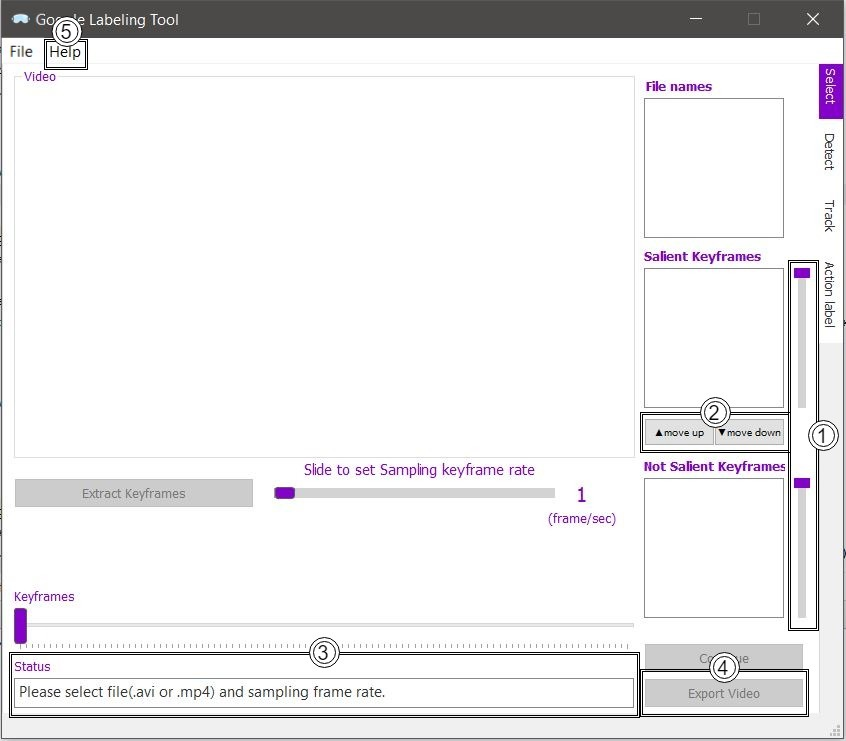
\includegraphics[scale=0.4]{chapter4/images/Final_ui/Select.jpg}
    \caption{รูปหน้าต่างแสดงผลของหน้าต่าง Select}
    \label{fig:final_select}
\end{figure}
จากรูปที่ \ref{fig:final_select} แสดงหน้าต่าง Select ของแอพพลิเคชั่น ซึ่งเมื่อเทียบกันกับหน้าต่าง Select ในฉบับร่าง (\ref{fig:}) จะมีส่วนที่เพิ่มเติมขึ้นมาดังนี้
\begin{enumerate}
	\item แถบเลื่อนสำหรับเลื่อนดูเฟรมที่มีมนุษย์ หรือ ไม่มีมนุษย์ เพื่อเพิ่มความสะดวกในการเลือกดูเฟรม
	\item ปุ่มสำหรับแก้ไขเฟรมที่มีมนุษย์หรือไม่มีมนุษย์
	\item แถบแสดงสถานะกระบวนการทำงาน
	\item ปุ่มสำหรับนำผลลัพธ์ออกเป็นไฟล์วิดิโอเฉพาะในช่วงที่มีมนุษย์อยู่
	\item แถบสำหรับคำแนะนำช่วยเหลือ
	\item ปุ่มสำหรับเปิดไฟล์
\end{enumerate}		

\clearpage
\subsection*{หน้าต่าง Detect}
\begin{figure}[!ht]
  \centering
    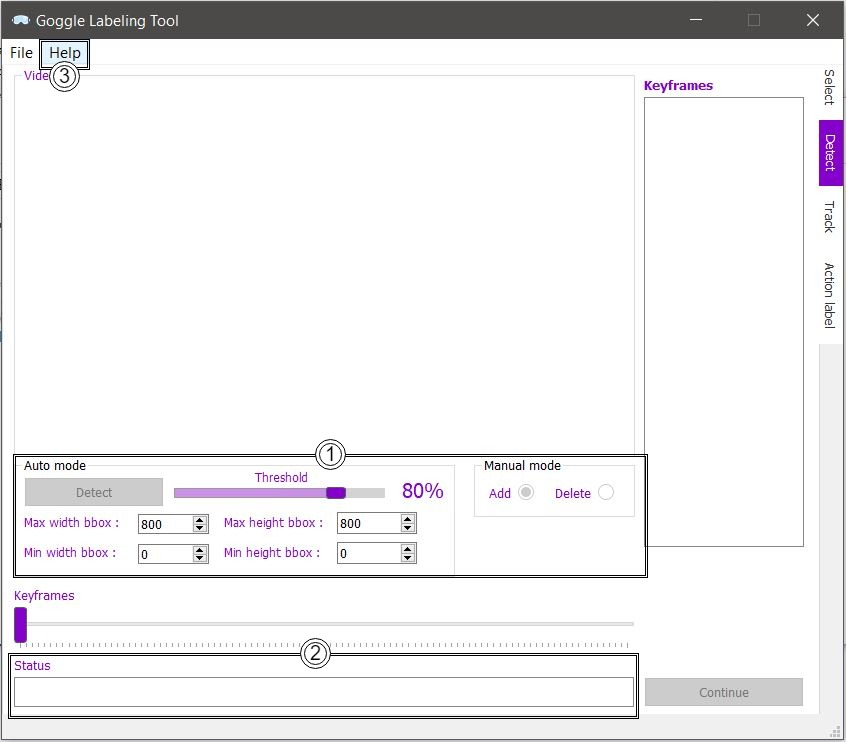
\includegraphics[scale=0.4]{chapter4/images/Final_ui/Detect.jpg}
    \caption{รูปหน้าต่างแสดงผลของหน้าต่าง Detect}
    \label{fig:final_detect}
\end{figure}
จากรูปที่ \ref{fig:final_detect} แสดงหน้าต่าง Detect ของแอพพลิเคชั่น ซึ่งเมื่อเทียบกันกับหน้าต่าง Detect ในฉบับร่าง (\ref{fig:}) จะมีส่วนที่เพิ่มเติมขึ้นมาดังนี้
\begin{enumerate}
	\item ปรับหน้าตาโหมดการทำงานแบบอัตโนมัติและกำหนดเองสามารถใช้งานได้สะดวกขึ้น และ เพิ่มความหลากหลายในการปรับแก้ไขการทำงานอัตโนมัติ
	\item แถบแสดงสถานะกระบวนการทำงาน
	\item แถบสำหรับคำแนะนำช่วยเหลือ
\end{enumerate}		

\clearpage
\subsection*{หน้าต่าง Track}
\begin{figure}[!ht]
  \centering
    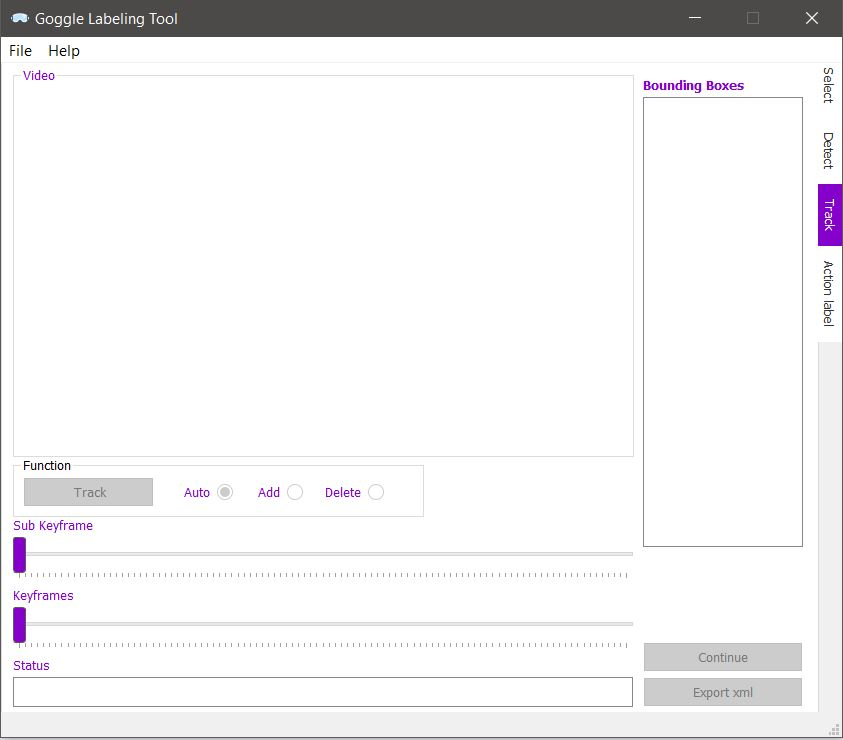
\includegraphics[scale=0.4]{chapter4/images/Final_ui/Track.jpg}
    \caption{รูปหน้าต่างแสดงผลของหน้าต่าง Track}
    \label{fig:final_track}
\end{figure}
จากรูปที่ \ref{fig:final_track} แสดงหน้าต่าง Track ของแอพพลิเคชั่น ซึ่งเมื่อเทียบกันกับหน้าต่าง Track ในฉบับร่าง (\ref{fig:}) จะมีส่วนที่เพิ่มเติมขึ้นมาดังนี้
\begin{enumerate}
	\item ปรับหน้าตาโหมดการทำงานแบบอัตโนมัติและกำหนดเองจากฉบับร่างเพื่อให้สามารถใช้งานได้สะดวกขึ้น
	\item เพิ่มแถบเลื่อน เป็น 2 แถบเลื่อนทำให้สามารถดูคีย์เฟรมและเฟรมที่อยู่ระหว่างช่วงคีย์เฟรมได้สะดวกขึ้น
	\item เพิ่มปุ่มสำหรับนำผลลัพธ์ออกเป็นไฟล์ XML 
	\item แถบแสดงสถานะกระบวนการทำงาน
	\item แถบสำหรับคำแนะนำช่วยเหลือ
\end{enumerate}		

\clearpage
\subsection*{หน้าต่าง Label}
\begin{figure}[!ht]
  \centering
    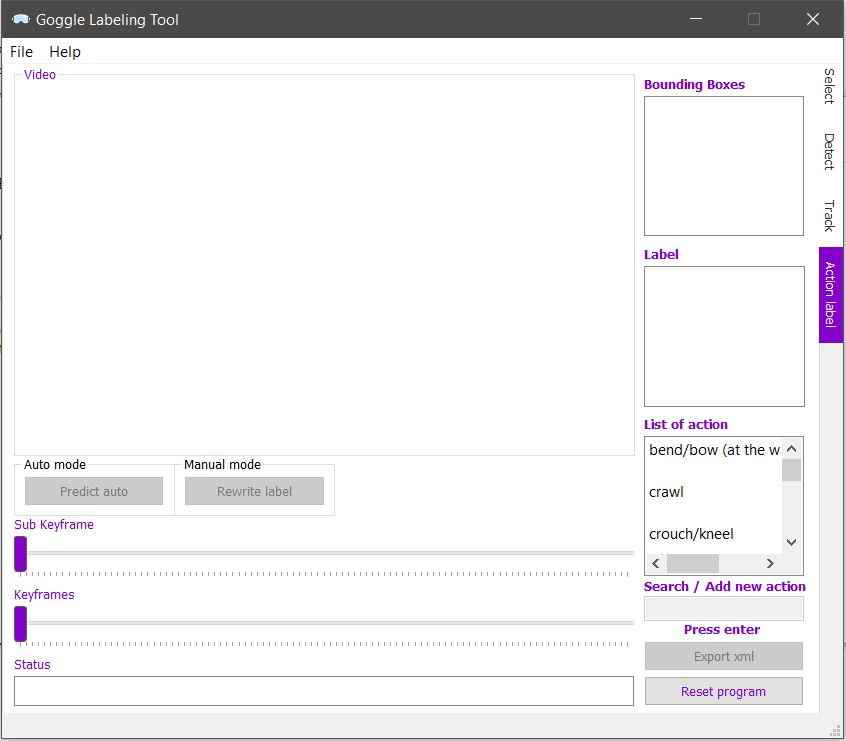
\includegraphics[scale=0.4]{chapter4/images/Final_ui/Label.jpg}
    \caption{รูปหน้าต่างแสดงผลของหน้าต่าง Label}
    \label{fig:final_label}
\end{figure}
จากรูปที่ \ref{fig:final_label} แสดงหน้าต่าง Label ของแอพพลิเคชั่น ซึ่งเมื่อเทียบกันกับหน้าต่าง Label ในฉบับร่าง (\ref{fig:}) จะมีส่วนที่เพิ่มเติมขึ้นมาดังนี้
\begin{enumerate}
	\item ปรับหน้าตาโหมดการทำงานแบบอัตโนมัติและกำหนดเองจากฉบับร่างเพื่อให้สามารถใช้งานได้สะดวกขึ้น
	\item เพิ่มแถบเลื่อน เป็น 2 แถบเลื่อนทำให้สามารถดูคีย์เฟรมและเฟรมที่อยู่ระหว่างช่วงคีย์เฟรมได้สะดวกขึ้น
	\item เครื่องมือสำหรับค้นหาหรือเพิ่มหมวดหมู่ของการกระทำ
	\item แถบแสดงสถานะกระบวนการทำงาน
	\item ปุ่มสำหรับเริ่มต้นการทำงานใหม่ 
	\item แถบสำหรับคำแนะนำช่วยเหลือ
\end{enumerate}		

\clearpage
\subsection{ผลลัพท์การทำงานในแต่ละหน้าต่างของแอพพลิเคชั่น}
\subsection*{ผลลัพท์การทำงานของหน้าต่าง Select}
\begin{figure}[!ht]
  \centering
    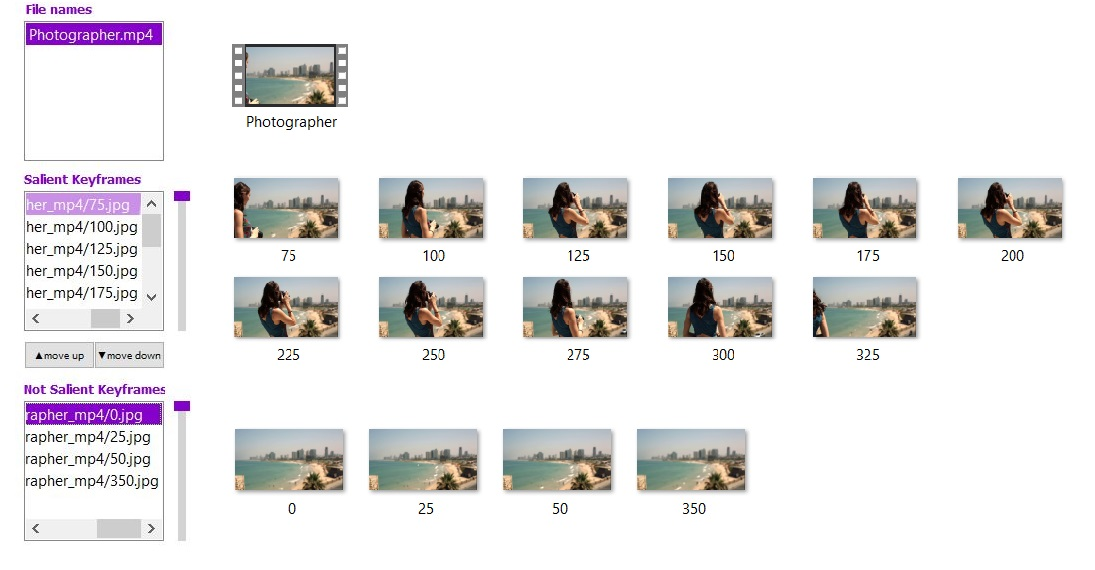
\includegraphics[scale=0.6]{chapter4/images/Result/result_select3.jpg}
    \caption{รูปผลลัพท์การแยกเฟรมที่มีมนุษย์อยู่และไม่มีมนุษย์อยู่ภายในเฟรม}
    \label{fig:result_select}
\end{figure}
ขั้นตอนแรกแอพพลิเคชั่นจะสกัดแยกวิดิโอออกเป็นเฟรมทั้งหมด และ ทำการสุ่มคีย์เฟรมออกมาตามความถี่ที่ผู้ใช้ตั้งไว้ จากนั้นแอพพลิเคชั่นจะนำโมเดล yolo-v3 มาตรวจสอบว่าแต่ละคีย์เฟรมมีเฟรมใดบ้างที่มีมนุษย์อยู่ภายในเฟรม จากนั้นจะทำการแยกเฟรมที่มีมนุษย์อยู่ และ ไม่มีมนุษย์อยู่ ดังรูป \ref{fig:result_select}


\subsection*{ผลลัพท์การทำงานของหน้าต่าง Detect}
\begin{figure}[!ht]
  \centering
    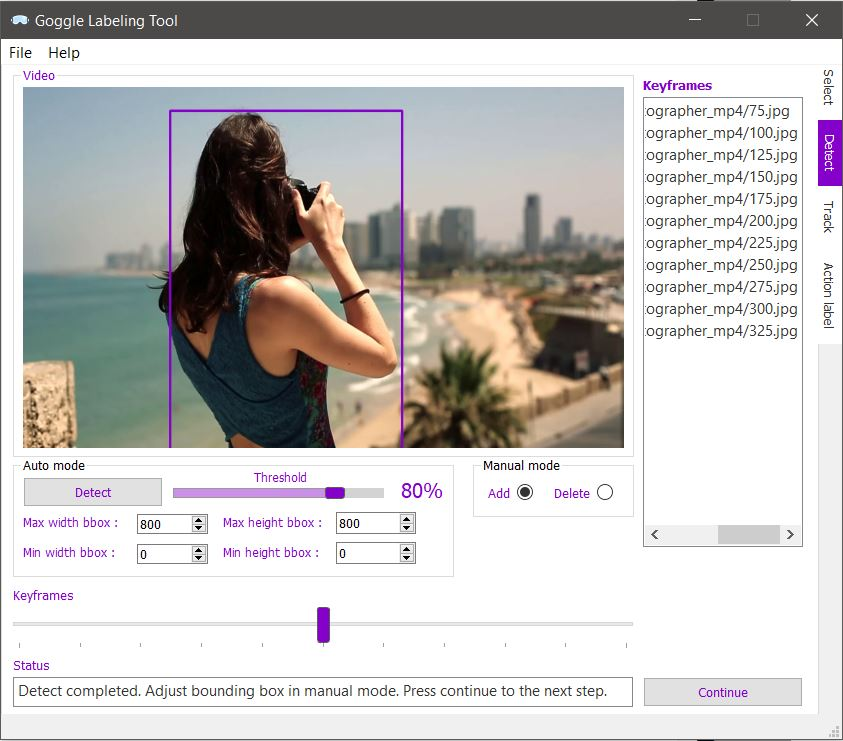
\includegraphics[scale=0.60]{chapter4/images/Result/result_select4.jpg}
    \caption{รูปคีย์เฟรมที่ถูกตีกรอบสี่เหลี่ยมในส่วนที่มีมนุษย์อยู่}
    \label{fig:result_detect}
\end{figure}
\clearpage
แอพพลิเคชั่นจะนำคีย์เฟรมที่มนุษย์ที่ได้จากหน้าต่าง Select นำมาตีกรอบสี่เหลี่ยมในส่วนของเฟรมที่มีมนุษย์อยู่โดยสามารถใช้โหมดการทำงานแบบอัตโนมัติหรือแบบแก้ไขเองก็ได้ ซึ่งผลลัพธ์ที่ได้จะได้คีย์เฟรมที่มีกรอบสี่เหลี่ยม ดังรูป \ref{fig:result_detect} จากนั้นจะบันทึกข้อมูลในไฟล์ .txt 

\subsection*{ผลลัพท์การทำงานของหน้าต่าง Track}
\begin{figure}[!ht]
    \centering
   \begin{subfigure}[b]{0.4\linewidth}
      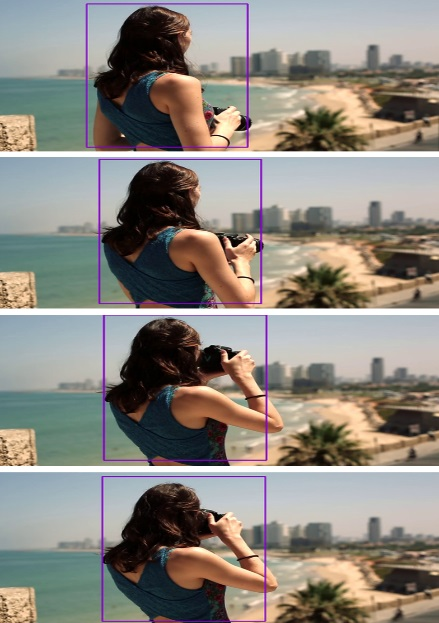
\includegraphics[width=\linewidth]{chapter4/images/Result/result_select6.jpg}
      \caption{ตัวอย่างเฟรมที่ถูกตีกรอบสี่เหลี่ยม}
    \end{subfigure}
\\
    \begin{subfigure}[b]{0.7\linewidth}
      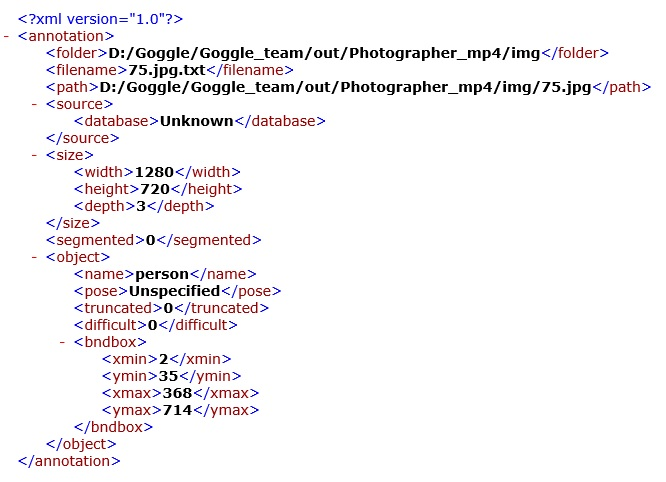
\includegraphics[width=\linewidth]{chapter4/images/Result/result_select7.jpg}
      \caption{ตัวอย่างไฟล์ XML}
    \end{subfigure}
    \caption{รูปผลลัพท์การทำงานของหน้าต่าง Track}
    \label{fig:result_track}
  \end{figure}
แอพพลิเคชั่นจะนำคีย์เฟรมที่ถูกตีกรอบสี่เหลี่ยมจากหน้าต่าง Detect มาทำนายกรอบสี่เหลี่ยมในเฟรมที่เหลือระหว่างช่วงคีย์เฟรม ซึ่งผลลัพธ์ที่ได้จะได้เฟรมทุกเฟรมที่มีมนุษย์อยู่ จะถูกตีกรอบสี่เหลี่ยม ดังรูป \ref{fig:result_track} จากนั้นสามารถบันทึกข้อมูลออกเป็นไฟล์ XML ได้ดังรูป

\clearpage
\subsection*{ผลลัพท์การทำงานของหน้าต่าง Label}
\begin{figure}[!ht]
    \centering
   \begin{subfigure}[b]{0.65\linewidth}
      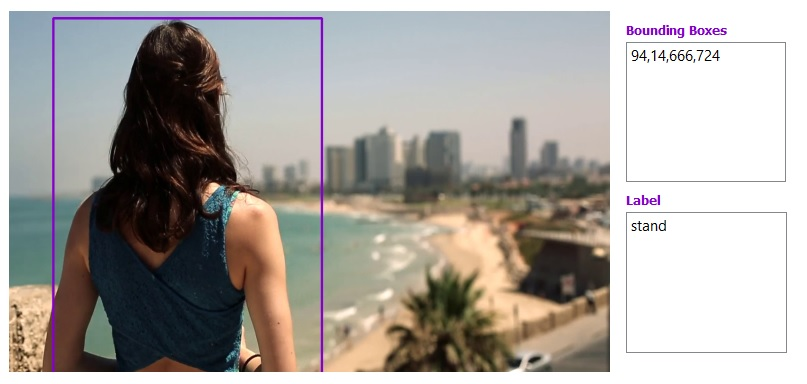
\includegraphics[width=\linewidth]{chapter4/images/Result/result_select.jpg}
      \caption{ตัวอย่างเฟรมที่ถูกตีกรอบสี่เหลี่ยมและคำทำนายการกระทำ}
    \end{subfigure}
\\
    \begin{subfigure}[b]{0.8\linewidth}
      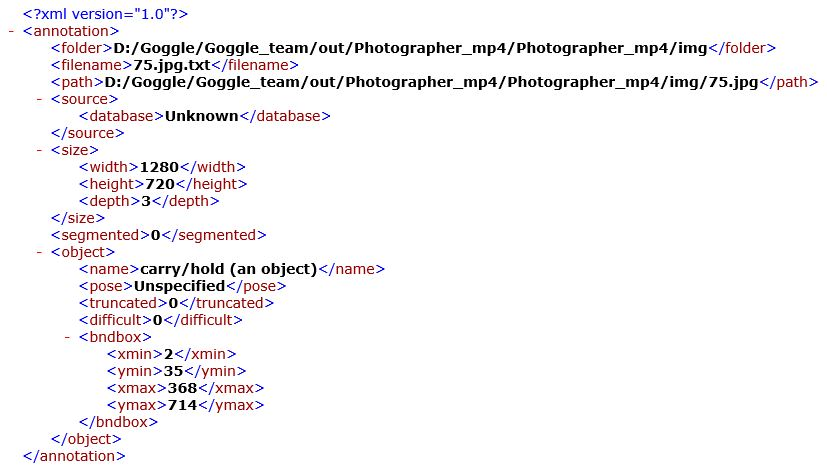
\includegraphics[width=\linewidth]{chapter4/images/Result/result_select9.jpg}
      \caption{ตัวอย่างไฟล์ XML}
    \end{subfigure}
    \caption{รูปผลลัพท์การทำงานของหน้าต่าง Label}
    \label{fig:result_track}
  \end{figure}
แอพพลิเคชั่นจะนำกรอบสี่เหลี่ยมของทุกเฟรมที่มีมนุษย์อยู่มาทำนายมนุษย์ในกรอบสี่เหลี่ยมนั้นกำลังมีการกระทำอะไรอยู่ โดยสามารถทำงานได้ทั้งโหมดอัตโนมัติหรือแบบแก้ไขเอง และสามารถบันทึกข้อมูลออกเป็นไฟล์ XML ได้ดังรูป


\clearpage
\section{ผลการทดลองการตรวจจับวัตถุ}
\subsection{ข้อมูลรายละเอียดประกอบการทดสอบ}
จำนวนเฟรมทั้งหมด: 20 เฟรม

\subsection{ทดสอบประสิทธิภาพการทำงานของโมเดลปัญญาประดิษฐ์สำหรับการทำการตรวจจับภาพบุคคล}
ข้อมูลผลการทำงานของโมเดลปัญญาประดิษฐ์สำหรับการทำการตรวจจับภาพบุคคล อ้างอิงข้อมูลจากเว็บไซต์ของ YOLO
\begin{table}[!ht]
	\begin{tabular}{|c|c|c|}
		\hline
		{}&{ความเร็วต่อรูปภาพ (มิลลิวินาที)}&{ความแม่นยำ (0.5 IoU mAP)}			\\
		\hline
		SSD Mobilenet v1 ppn	 		& 26				& 20														\\
		YOLO-v3 320				& 22				& 51.5				\\	
		YOLO-v3 tiny				& 4.5				& 33.1				\\
		YOLO-v3 spp				& 50				& 60.6				\\	
		Faster RCNN inceptrion v2		& 58				& 28		\\
	\hline
	\end{tabular}
\end{table}

ข้อมูลผลการทำงานของโมเดลปัญญาประดิษฐ์สำหรับการทำการตรวจจับภาพบุคคลหลังจากทำการทดลอง
\begin{table}[!ht]
	\begin{tabular}{|c|c|c|}
		\hline 
		{}&{ความเร็วต่อรูปภาพ (มิลลิวินาที)}&{ความแม่นยำ (0.5 IoU mAP)}			\\
		\hline
		SSD Mobilenet v1 ppn	 					& 63 			& 37			\\
		YOLO-v3 320							& 65			& 64.9		\\
		YOLO-v3 tiny							& 17			& 44.4			\\
		YOLOv3-spp							& 65			& 70.3			\\	
		Faster RCNN inceptrion v2					& 981		& 42.5		\\
		\hline
	\end{tabular}
\end{table}
จำนวนมนุษย์ที่อยู่ในเฟรม : 0-5 คน

ความละเอียดรูปภาพ : 1280 \texttimes 720  พิกเซล

ขอบเขตอัตราส่วนร่วมของกรอบที่เหลี่ยมที่จะนับว่าการทำนายถูกต้อง: 50\% ขึ้นไป

\subsubsection*{ข้อมูลความเที่ยงตรงของโมเดลปัญญาประดิษฐ์}
\begin{table}[!ht]
    \centering
	\begin{tabular}{|c|c|c|}
			\hline
			{}&{ความเร็วต่อรูปภาพ(มิลลิวินาที)}&{ความเที่ยงตรง (0.5 IOU mAP)}			\\
			\hline
			SSD Mobilenet v1 ppn	 		& 26				& 20														\\
			YOLOv3-320				& 22				& 51.5				\\	
			YOLOv3-tiny				& 4.5				& 33.1				\\
			YOLOv3-spp				& 50				& 60.6				\\	
			Faster rcnn inceptrionv2		& 58				& 28		\\
		\hline
	\end{tabular}
	\caption{ข้อมูลผลการทำงานของโมเดลปัญญาประดิษฐ์สำหรับการทำการตรวจจับภาพบุคคล อ้างอิงข้อมูลจากเว็บไซต์ของ yolo}
    	\label{tab:origina_detectEx}
\end{table}


\subsection{ทดสอบประสิทธิภาพการทำงานของโมเดลปัญญาประดิษฐ์สำหรับการทำการตรวจจับภาพบุคคล}
\subsubsection*{ข้อมูลความแม่นยำของโมเดลปัญญาประดิษฐ์เมื่อทดสอบด้วยชุดข้อมูลของผู้วิจัย}
\begin{table}[!ht]
	\centering
	\begin{tabular}{|c|c|c|}
			\hline 
			{}&{ความเร็วต่อรูปภาพ(มิลลิวินาที)}&{ความแม่นยำ (0.5 IOU)}			\\
			\hline
			SSD Mobilenet v1 ppn	 					& 63 			& 37			\\
			YOLOv3-320							& 65			& 64.9		\\
			YOLOv3-tiny							& 17			& 44.4			\\
			YOLOv3-spp							& 65.4			& 70.3			\\	
			Faster rcnn inceptrionv2					& 981		& 42.5		\\
		\hline
	\end{tabular}
	\caption{ข้อมูลผลการทำงานของโมเดลปัญญาประดิษฐ์สำหรับการทำการตรวจจับภาพบุคคลหลังจากทำการทดลอง}
    \label{tab:origina_detectEx}
\end{table}

\clearpage
\section{ผลการทดสอบระบบติดตามตำแหน่งของมนุษย์}
\subsection{ข้อมูลรายละเอียดประกอบการทดสอบ}
ชื่อวิดีโอ: Photographer beach photography

ความยาววิดีโอ: 15 วินาที

จำนวนเฟรมทั้งหมด: 374 เฟรม

อัตราเฟรมต่อวินาที: 24.9 เฟรมต่อวินาที

ความละเอียดของวิดีโอ: 1920\texttimes 1080 พิกเซล

ความละเอียดของวิดีโอที่ใช้ในการประมวลผลจริง: 1280\texttimes 720 พิกเซล

ขอบเขตอัตราส่วนร่วมของกรอบที่เหลี่ยมที่จะนับว่าการทำนายถูกต้อง: 80\% ขึ้นไป

\subsection{ผลทดสอบประสิทธิภาพ และความเร็วในการประมวลผล}
\begin{table}[!ht]
    \centering
    \begin{tabular}{|c|c|c|c|c|}
        \hline
        วิธีการทดสอบ & \multicolumn{2}{c|}{ความแม่นยำ (\%)} & \multicolumn{2}{c|}{ความเร็วในการประมวลผล (วินาที)}\\
        \hline
        \begin{tabular}{@{}l@{}}ใช้โมเดลปัญญาประดิษฐ์ YOLO-v3 spp \\ ประมวลผลทุกเฟรมในวิดีโอ\end{tabular} & 95 & - & 452 & -\\
        \hline
        \begin{tabular}{@{}l@{}}ใช้โมเดลปัญญาประดิษฐ์ YOLO-v3 spp \\ ประมวลผลทุกๆ N เฟรมในวิดีโอ \\แล้วใช้ระบบติดตามการเคลื่อนไหวตำแหน่งต่อไปของ\\วัตถุในเฟรมระหว่างนั้น\end{tabular} & \multicolumn{1}{c}{} & \multicolumn{1}{c}{} & \multicolumn{1}{c}{} & \multicolumn{1}{c|}{}\\ 
        \hline    
        \multicolumn{1}{|l|}{N = 10} & 85 & -10 & 69 & -383\\
        \multicolumn{1}{|l|}{N = 20} & 80 & -15 & 41 & -411\\
        \multicolumn{1}{|l|}{N = 25} & 75 & -20 & 35 & -417\\
        \hline
    \end{tabular}
    \caption{ผลการทดสอบประสิทธิภาพของการตรวจจับกรอบสี่เหลี่ยมภายในวิดีโอ}
    \label{tab:trackEx}
\end{table}
จากตารางที่ \ref{tab:trackEx} ผู้วิจัยได้ทำการทดสอบความแม่นยำและความเร็วในการประมวลผลของการใช้โมเดลปัญญาประดิษฐ์ YOLO-v3 spp ประมวลผลทุกเฟรม 
แม้จะตั้งขอบเขตอัตราส่วนร่วมของกรอบที่เหลี่ยมที่จะนับว่าการทำนายถูกต้องสูงถึง 80\% แต่ความแม่นยำยังสูงถึง 95\% ใช้เวลาในการประมวลผล 452 วินาที 
เฉลี่ยเฟรมละ 1.2 วินาที ซึ่งถือเป็นความแม่นยำที่สูงมากเมื่อเทียบกับเวลาที่ใช้ในการประมวล

ต่อมาเป็นการทดสอบโดยใช้โมเดลปัญญาประดิษฐ์ประมวลผลเฉพาะบางเฟรมทุกๆช่วงหนึ่ง แล้วใช้ระบบติดตามการเคลื่อนไหวตำแหน่งต่อไปของวัตถุในการสร้างกรอบสี่เหลี่ยมในเฟรมระหว่างนั้น เพื่อเพิ่มความเร็วในการประมวลผล 
โดยระยะที่ใช้ในการทดสอบคือ ทุกๆ 10 เฟรม 20 เฟรม และ 25 เฟรม ซึ่งจากผลการทดสอบนั้นพบว่าวิธีการนี้มีความแม่นแปรผกผันกับจำนวนเฟรมที่ใช้ในการประมวลผล (จำนวนเฟรมมากขึ้นจะทำให้ความแม่นยำต่ำลง) 
และความเร็วในการประมวลผลนั้นจะแปรผันตรงกับจำนวนเฟรมที่ใช้ในการประมวลผล (จำนวนเฟรมมากขึ้นจะทำให้ประมวลผลเร็วขึ้น) โดยที่การใช้ระยะประมวลผลเป็น 10 เฟรมนั้นใช้เวลาในการประมวลผลเพียง 69 วินาที 
น้อยกว่าการใช้โมเดลปัญญาประดิษฐ์ YOLO-v3 spp ประมวลผลทุกเฟรมถึง 383 วินาที ซึ่งเร็วกว่าถึง 6.5 เท่า และความแม่นยำลดลงมาเหลือ 85\% น้อยกว่าอยู่เพียง 10\% เท่านั้น ถือเป็นความแม่นยำที่สูงเมื่อเทียบกันด้วยระยะเวลาในการประมวลผล
ในขณะที่การใช้ระยะประมวลผล 20 เฟรมนั้นจะประมวลผลเร็วกว่าการใช้โมเดลปัญญาประดิษฐ์ YOLO-v3 spp ประมวลผลทุกเฟรมถึง 11 เท่า และมีความแม่นยำต่ำกว่า 15\%
และเมื่อใช้ระยะประมวลผล 25 เฟรมจะเร็วกว่าประมาณ 13 เท่า และความแม่นยำต่ำลงถึง 20\% 

\section{ผลการทดสอบระบบระบุตัวตนของมนุษย์}
\subsection{ทดสอบประสิทธิ์ภาพการทำงานของโมเดลปัญญาประดิษฐ์สำหรับการระบุตัวตนของบุคคล}
ความแม่นยำของโมเดลปัญญาประดิษฐ์จากแหล่งที่มีมามีค่าดังตารางด้านล่างดังนี้
\begin{table}[!ht]
\centering
\begin{tabular}{|c|c|}
		\hline
		{โมเดลปัญญาประดิษฐ์}&{rank1/mAP โดยใช้วิธีการทดสอบด้วย Global+DMLI}				\\
		\hline
		ResNet50 Market1501	 			& 91.0/77.6								\\
		ResNet50 DukeMTMCReID			& 80.7/68.0								\\
		ResNet50 CUHK03				& 60.9/59.7								\\
		ResNet50 MSMT17				& 66.3/40.6								\\
	\hline
\end{tabular}
\caption{ผลการทดสอบความแม่นยำของโมเดลปัญญาประดิษฐ์}
\label{tab: Accuracy of model ReID}
\end{table}
ต่อมานำโมเดลปัญญาประดิษฐ์แต่ละอันมาทดสอบกับตัวอย่างภาพชุดข้อมูลที่ทางคณะผู้วิจัยได้สร้างขึ้น โดยภาพชุดข้อมูลที่นำมาใช้จะผ่านการตรวจหาบุคคลภายในภาพด้วยโมเดลปัญญาประดิษฐ์ YoLo v3 320
\begin{figure}[!ht]
    \centering
    \begin{subfigure}[b]{0.2\textwidth}
        \centering
        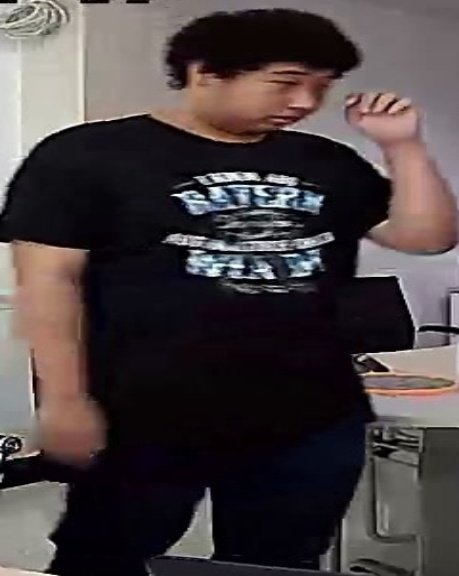
\includegraphics[width=\textwidth]{chapter4/images/o_0.jpg}
        \label{fig:ex_1}
    \end{subfigure}
    \begin{subfigure}[b]{0.2\textwidth}
        \centering
        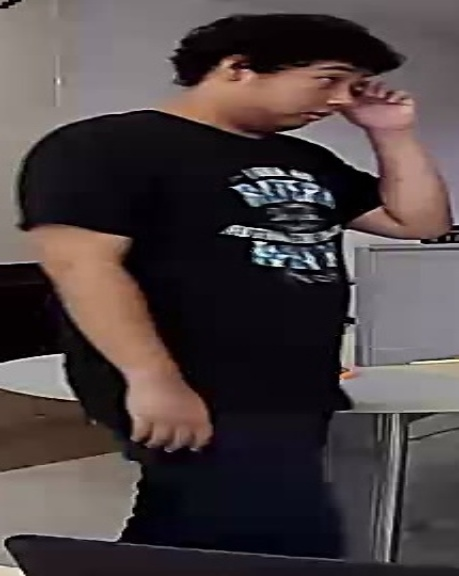
\includegraphics[width=\textwidth]{chapter4/images/o_1.jpg}
        \label{fig:ex_2}
    \end{subfigure}
    \caption{ภาพตัวอย่างชุดข้อมูลสำหรับการทดลองครั้งที่ 1}
    \label{fig: ภาพตัวอย่างชุดข้อมูลสำหรับการทดลอง 1}
\end{figure}
\begin{table}[!ht]
\centering
\begin{tabular}{|c|c|}
		\hline
		{โมเดลปัญญาประดิษฐ์}&{ความแม่นยำในการระบุบุคคล}							\\
		\hline
		ResNet50 Market1501	 			& 0.4308								\\
		ResNet50 DukeMTMCReID			& 0.4827								\\
		ResNet50 CUHK03				& 0.4914								\\
		ResNet50 MSMT17				& 0.4668								\\
	\hline
\end{tabular}
\caption{ผลการทดสอบความแม่นยำสำหรับการระบุบุคคลของโมเดลปัญญาประดิษฐ์ครั้งที่ 1}
\label{tab: Original distant of image 1}
\end{table}
\begin{figure}[!ht]
    \centering
    \begin{subfigure}[b]{0.2\textwidth}
        \centering
        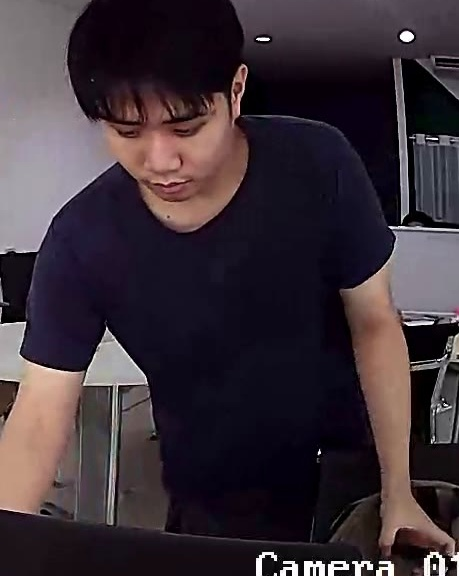
\includegraphics[width=\textwidth]{chapter4/images/first_0.jpg}
        \label{fig:ex_3}
    \end{subfigure}
    \begin{subfigure}[b]{0.2\textwidth}
        \centering
        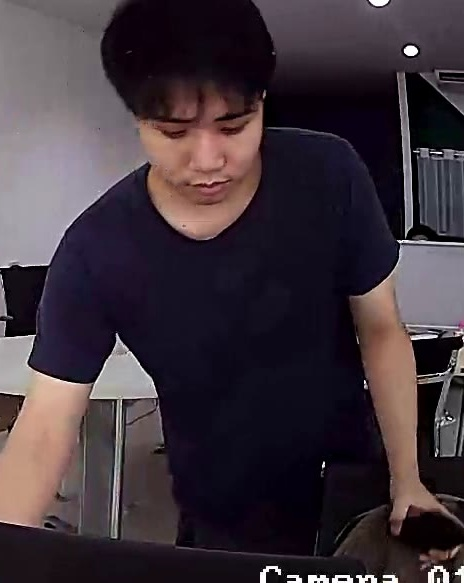
\includegraphics[width=\textwidth]{chapter4/images/first_1.jpg}
        \label{fig:ex_4}
    \end{subfigure}
    \caption{ภาพตัวอย่างชุดข้อมูลสำหรับการทดลองครั้งที่ 2}
    \label{fig: ภาพตัวอย่างชุดข้อมูลสำหรับการทดลอง 2}
\end{figure}
\begin{table}[!ht]
\centering
\begin{tabular}{|c|c|}
		\hline
		{โมเดลปัญญาประดิษฐ์}&{ความแม่นยำในการระบุบุคคล}							\\
		\hline
		ResNet50 Market1501	 			& 0.3035								\\
		ResNet50 DukeMTMCReID			& 0.3332								\\
		ResNet50 CUHK03				& 0.3	042								\\
		ResNet50 MSMT17				& 0.3684								\\
	\hline
\end{tabular}
\caption{ผลการทดสอบความแม่นยำสำหรับการระบุบุคคลของโมเดลปัญญาประดิษฐ์ครั้งที่ 2}
\label{tab: Original distant of image 2}
\end{table}
\clearpage
\begin{figure}[!ht]
    \centering
    \begin{subfigure}[b]{0.2\textwidth}
        \centering
        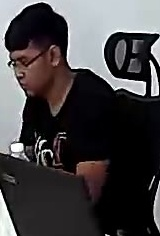
\includegraphics[width=\textwidth]{chapter4/images/fei_0.jpg}
        \label{fig:ex_5}
    \end{subfigure}
    \begin{subfigure}[b]{0.2\textwidth}
        \centering
        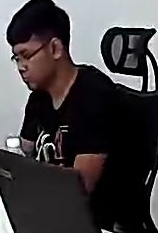
\includegraphics[width=\textwidth]{chapter4/images/fei_1.jpg}
        \label{fig:ex_6}
    \end{subfigure}
    \caption{ภาพตัวอย่างชุดข้อมูลสำหรับการทดลองครั้งที่ 3}
    \label{fig: ภาพตัวอย่างชุดข้อมูลสำหรับการทดลอง 3}
\end{figure}
\begin{table}[!ht]
\centering
\begin{tabular}{|c|c|}
		\hline
		{โมเดลปัญญาประดิษฐ์}&{ความแม่นยำในการระบุบุคคล}							\\
		\hline
		ResNet50 Market1501	 			& 0.3308								\\
		ResNet50 DukeMTMCReID			& 0.3296								\\
		ResNet50 CUHK03				& 0.3	134								\\
		ResNet50 MSMT17				& 0.3968								\\
	\hline
\end{tabular}
\caption{ผลการทดสอบความแม่นยำสำหรับการระบุบุคคลของโมเดลปัญญาประดิษฐ์ครั้งที่ 3}
\label{tab: Original distant of image 3}
\end{table}
ค่าความแม่นยำในการระบุบุคคลนั้นค่ายิ่งเข้าใกล้ 0 แสดงบุคคลใน 2 เฟรมนั้นเป็นบุคคลเดียวกัน จากการทดลองครั้งที่ 1 จะเป็นเฟรมที่ไม่ต่อเนื่องกัน การทดลองครั้งที่ 2 และ 3 นั้นจะเป็นเฟรมที่ต่อเนื่องกันมากขึ้นตามลำดับ ซึ่งจะแสดงให้เห็นว่าโมเดลปัญญาประดิษฐ์ที่สามารถให้ผลลัพท์ที่มีประสิทธิภาพต่อเนื่องมากที่สุดคือ ResNet50 Market1501


\section{ผลการทดสอบการจดจำการกระทำของมนุษย์}
\subsection{ทดสอบประสิทธิภาพการทำงานของโมเดลปัญญาประดิษฐ์ Resnet50 ที่ถูกสร้างด้วยชุดข้อมูลของ AVA โดยใช้ชุดข้อมูลของ AVA ในการทดสอบและเทียบผลลัพธ์กับแหล่งอ้างอิง ได้ผลการทดลองดังตารางต่อไปนี้}
\begin{table}[!ht]
	\centering
	\begin{tabular}{|c|c|c|}
			\hline
			{}&{ความเร็วต่อรูปภาพ(มิลลิวินาที)}&{ความแม่นยำ (PASCAL mAP)}			\\
			\hline
			แหล่งอ้างอิง	 					& 93.00		& 0.110				\\
			ผลการทดสอบของผู้วิจัย				& 85.35  	& 0.068				\\
			\hline
	\end{tabular}
\caption{ผลการทดสอบความแม่นยำของโมเดลปัญญาประดิษฐ์เทียบผลลัพธ์กับแหล่งอ้างอิง}
\label{tab: Compare PASCAL mAP with source}
\end{table}
ความเร็วของต่อรูปภาพทางผู้วิจัยได้ใช้กราฟิกการ์ด GTX 2080 Ti ในการทดสอบซึ่งจะให้ความเร็วอยู่ที่ 85.35 มิลลิวินาที/ภาพ ซึ่งทางแหล่งอ้างอิงนั้นใช้กราฟิกการ์ด Nvidia GeForce GTX TITAN X 
ในส่วนของค่าความแม่นยำที่ไม่เท่ากัน คาดว่าจะเป็นเพราะการประมวลผลของกราฟิกการ์ดของรุ่นที่ต่างกันและสเปคของเครื่องคอมพิวเตอร์จึงทำให้ค่า mAP ที่ออกมาไม่เท่ากัน

\subsection{ทดสอบประสิทธิภาพการทำงานของโมเดลปัญญาประดิษฐ์ Resnet50 ที่เคยถูกสร้างด้วยชุดข้อมูลของ AVA และใช้ชุดข้อมูลที่ผู้วิจัยสร้างขึ้นในการทดสอบและเทียบผลลัพธ์กับแหล่งอ้างอิง}
\begin{table}[!ht]
	\centering
	\begin{tabular}{|c|c|c|}
			\hline
			{}&{ความเร็วต่อรูปภาพ(มิลลิวินาที)}&{ความแม่นยำ (PASCAL mAP)}			\\
			\hline
			แหล่งอ้างอิง	 					& 93.00			& 0.110			\\
			ผลการทดสอบของผู้วิจัย				& 63.11			& 0.152			\\
			\hline
	\end{tabular}
\caption{ผลการทดสอบความแม่นยำของโมเดลปัญญาประดิษฐ์ เมื่อใช้กับชุดข้อมูลที่ผู้วิจัยสร้างขึ้น}
\label{tab: Compare PASCAL mAP with dataset created by the researcher}
\end{table}
ความเร็วของต่อรูปภาพทางผู้วิจัยได้ใช้กราฟิกการ์ด Tesla V100-SXM2 ในการทดสอบซึ่งจะให้ความเร็วอยู่ที่ 63.11 มิลลิวินาที/ภาพ ซึ่งทางแหล่งอ้างอิงนั้นใช้กราฟิกการ์ด Nvidia GeForce GTX TITAN X ซึ่งการนำโมเดลปัญญาประดิษฐ์ AVA มาใช้ในการทดสอบกับชุดข้อมูลทดสอบที่ทางผู้วิจัยสร้างขึ้น ซึ่งผลลัพธ์ที่ได้ออกมานั้นสูงขึ้นหากเทียบการทดลองจากแหล่งอ้างอิง ทำให้การตั้งสมมติฐานที่ตั้งไว้ตอนแรกนั้นไม่ถูกต้อง ในส่วนที่ชุดข้อมูลที่ทางผู้วิจัยได้สร้างขึ้นจะมีการตัดหมวดหมู่ที่ไม่มีในชุดข้อมูลของ AVA ออกไป ดังนั้นจึงทำให้ผู้วิจัยสรุปได้ว่าการนำโมเดลปัญญาประดิษฐ์ของ AVA มาใช้กับชุดข้อมูลที่มีหมวดหมู่ไม่ครบก็สามารถทำงานได้มีประสิทธิภาพสูงกว่าแหล่งอ้างอิง
\clearpage
\subsection{ทดสอบประสิทธิภาพการทำงานของโมเดลปัญญาประดิษฐ์ Resnet50 ที่ถูกสร้างด้วยชุดข้อมูลที่ผู้วิจัยสร้างขึ้น และใช้ชุดข้อมูลที่ผู้วิจัยสร้างขึ้นในการทดสอบและเทียบผลลัพธ์การทดสอบก่อนหน้า}
ในส่วนนี้จะเป็นการทดสอบโดยใช้โครงสร้างโมเดลปัญญาประดิษฐ์เป็น ResNet50 โดยจะมีการใช้ชุดข้อมูลที่ผู้วิจัยสร้างขึ้นซึ่งเป็นชุดข้อมูลทดสอบเดียวกับที่ทางผู้วิจัยใช้ในการทดสอบโมเดลปัญญาประดิษฐ์ AVA มาใช้ในการทำสอบครั้งนี้ด้วย โดยชุดข้อมูลที่นำมาใช้สำหรับการสร้างโมเดลปัญญาประดิษฐ์จะมีอยู่ 2 ชุดข้อมูล ซึ่งได้แก่ goggle dataset v1 และ goggle dataset v2 ชุดข้อมูลทั้งสองอันนี้จะแตกต่างกันตรงที่ goggle dataset v2 นั้นเป็นชุดข้อมูลเกิดจากการที่ทางผู้วิจัยได้เข้าไปลบในส่วนที่มีการกำกับข้อมูลภาพผิดและมีการสุ่มตัวอย่างของข้อมูลออกมาเพื่อลดโอกาสที่จะเกิด overfitting ของข้อมูล โดยจำนวนชุดข้อมูลของ goggle dataset v1 ที่ใช้สำหรับการสร้างโมเดลจะมี 213,061 ภาพ และในส่วนของ goggle dataset v2 จะมีจำนวนชุดข้อมูล 120,177 ภาพ และมีการตั้งค่าตัวแปรต่าง ๆ ที่ใช้สำหรับการสร้างโมเดลปัญญาประดิษฐ์ดังนี้
\begin{enumerate}
	\item ขนาดของรูปภาพ : 224x224
	\item Pooling : Average pooling
	\item Activation function : Softmax
	\item Epoch : 50
	\item Batch size : 16
	\item Optimize : Momentum
	\begin{enumerate}
		\item Learning rate : 0.001
		\item Momentum : 0.9
	\end{enumerate}
\end{enumerate}
\subsubsection{การทดสอบสร้างโมเดลปัญญาประดิษฐ์ ResNet50 ด้วยชุดข้อมูล goggle dataset v1 และ goggle dataset v2}
\begin{table}[!ht]
	\centering
	\begin{tabular}{|c|c|c|}
			\hline
			{ชุดข้อมูล}&{ความเร็วต่อรูปภาพ(มิลลิวินาที)}&{ความแม่นยำ (PASCAL mAP)}			\\
			\hline
			goggle dataset v1 ResNet50			& 2.78			& 0.279				\\
			goggle dataset v2 ResNet50			& 2.52			& 0.294				\\
			\hline
	\end{tabular}
\caption{ผลการทดสอบความแม่นยำของโมเดลปัญญาประดิษฐ์ที่ผู้วิจัยสร้างขึ้น ใช้กับชุดข้อมูลที่ผู้วิจัยสร้างขึ้น}
\label{tab: Test PASCAL mAP of dataset created by the researcher}
\end{table}
จากตาราง \ref{tab: Test PASCAL mAP of dataset created by the researcher} การทดลองจะเป็นได้ว่าความเร็วของต่อรูปภาพทางผู้วิจัยได้ใช้กราฟิกการ์ด Tesla V100-SXM2 แต่ความเร็วนั้นเร็วกว่าตอนที่ทดสอบด้วยโมเดลปัญญาประดิษฐ์ AVA เป็นอย่างมาก เนื่องจากโมเดลปัญญาประดิษฐ์ของ AVA นั้นจะมีการทำในส่วนของการหากรอบสี่เหลี่ยมรอบตัวมนุษย์ด้วย ในขณะที่โมเดลปัญญาประดิษฐ์ของผู้วิจัยนั้นจะไม่มีการหากรอบสี่เหลี่ยมรอบตัวมนุษย์ เพราะจะมีการนำโมเดลปัญญาประดิษฐ์ของ YOLO-v3 spp มาหากรอบสี่เหลี่ยมรอบตัวมนุษย์ตั้งแต่แรกแล้ว ในส่วนของค่า mAP ที่ได้ออกมานั้น goggle dataset v2 มีค่า mAP มากกว่า แต่มีความแตกต่างกันไม่มาก อาจจะเป็นไปได้ว่าเพราะจำนวนข้อมูลที่น้อยกว่า goggle dataset v1 ดังนั้นทางผู้วิจัยจึงได้เลือก goggle dataset v2 มาใช้กับการทดลองครั้งต่อไป
\clearpage
\subsubsection{การทดสอบสร้างโมเดลปัญญาประดิษฐ์ ResNet50 ด้วยชุดข้อมูล goggle dataset v2 โดยใช้ weight ของ ImageNet}
\begin{table}[!ht]
	\centering
	\begin{tabular}{|c|c|c|}
			\hline
			{}&{ความเร็วต่อรูปภาพ(มิลลิวินาที)}&{ความแม่นยำ (PASCAL mAP)}			\\
			\hline
			ResNet50-ImageNet			& 2.51			& 0.454				\\
			\hline
	\end{tabular}
\caption{ผลการทดสอบความแม่นยำของโมเดลปัญญาประดิษฐ์ที่ผู้วิจัยสร้างขึ้นโดยใช้ weight จาก ImageNet ใช้กับชุดข้อมูลที่ผู้วิจัยสร้างขึ้น}
\label{tab: Test PASCAL mAP of dataset created by the researcher and pretrain weight imagenet}
\end{table}
จากตาราง \ref{tab: Test PASCAL mAP of dataset created by the researcher and pretrain weight imagenet} เมื่อทางผู้วิจัยได้นำ weight ของ ImageNet มาช่วยในการสร้างโมเดลทำให้ประสิทธิภาพของโมเดลที่ได้ออกมานั้นสูงขึ้นมากเมื่อเทียบกับการทดสอบโมเดลปัญญาประดิษฐ์ของผู้วิจัยก่อนหน้านี้

\subsubsection{การทดสอบสร้างโมเดลปัญญาประดิษฐ์ ResNet50-ImageNet ด้วยชุดข้อมูล goggle dataset v2 ด้วยวิธีการทำ scaling}
\begin{table}[!ht]
	\centering
	\begin{tabular}{|c|c|c|}
			\hline
			{}&{ความเร็วต่อรูปภาพ(มิลลิวินาที)}&{ความแม่นยำ (PASCAL mAP)}			\\
			\hline
			ResNet50-ImageNet	 Normalization				& 2.51			& 0.449				\\
			ResNet50-ImageNet	 Centering Featurewise		& 2.40			& 0.457				\\
			ResNet50-ImageNet	 Centering Samplewise		& 2.49			& 0.466				\\
			ResNet50-ImageNet	 Standardize Featurewise		& 2.48			& 0.407				\\
			ResNet50-ImageNet	 Standardize Samplewise		& 2.49			& 0.432				\\
			\hline
	\end{tabular}
\caption{ผลการทดสอบความแม่นยำของโมเดลปัญญาประดิษฐ์ที่ผู้วิจัยสร้างขึ้นโดยใช้ weight จาก ImageNet และการทำ scaling ใช้กับชุดข้อมูลที่ผู้วิจัยสร้างขึ้น}
\label{tab: Test PASCAL mAP of dataset created by the researcher with pretrain weight imagenet and scaling}
\end{table}

จากตาราง \ref{tab: Test PASCAL mAP of dataset created by the researcher with pretrain weight imagenet and scaling} จะเป็นการทดลอง scaling ด้วยรูปแบบต่าง อย่างการทำ normalization จะเป็นทำให้ค่าในพิกเซลอยู่ในช่วง 0 ถึง 1 การทำ centering คือการลบค่าในพิกเซลด้วยค่าเฉลี่ยของพิกเซล โดยจะแบ่งออกเป็น 2 แบบได้แก่ featurewise และ samplewise โดย featurewise จะเป็นการหาค่าเฉลี่ยพิกเซลจากทุกรูปในชุดข้อมูลแล้วนำมาลบออกในแต่ละพิกเซลของรูป ส่วนของ samplewise จะไม่มีการไปยุ่งเกี่ยวกับรูปอื่น คือจะหาค่าเฉลี่ยของพิกเซลของรูปนั้น ๆ และนำค่าพิกเซลในรูปนั้น ๆ ลบออกด้วยค่าเฉลี่ย ต่อมาการทำ standardize คือการหารค่าในพิกเซลด้วยค่า standard deviation ของพิกเซลในรูป ซึ่งจะแบ่งออกเป็น 2 แบบ ได้แก่ featurewise และ samplewise เหมือนกับ centering โดย featurewise จะหาค่า standard deviation ของทุกพิกเซลในชุดข้อมูลแล้วนำมาหารในแต่ละพิกเซลของรูป ส่วนของ samplewise จะเป็นการหาค่า standard deviation ของรูปนั้น ๆ มาหารกับทุกพิกเซลในรูปนั้น ๆ จากการทำลองจะทำให้เห็นว่าโมเดลปัญญาประดิษฐ์ที่มีประสิทธิภาพสูงที่สุดคือโมเดลปัญญาประดิษฐ์ ResNet50-ImageNet	 Centering Samplewise
\clearpage
\subsubsection{การทดสอบ average preicision (AP) ของโมเดลปัญญาประดิษฐ์ ResNet50-ImageNet Centering Samplewise}
\begin{table}[!ht]
	\centering
	\begin{tabular}{|c|c|c|}
			\hline
			{Label}&{ResNet50-ImageNet Centering Samplewise}			\\
			\hline
			Play phone				& 0.824			\\
			Eat						& 0.975			\\
			Sit						& 0.215			\\
			Sleep					& 0.473			\\
			Stand					& 0.043			\\
			Walk					& 0.266			\\
			\hline
	\end{tabular}
\caption{โมเดลปัญญาประดิษฐ์ ResNet50-ImageNet	 Centering Samplewise วัดค่า average precision (AP) ของแต่ละหมวดหมู่}
\label{tab: ResNet50-ImageNet Centering Samplewise average precision}
\end{table}

จากตาราง \ref{tab: ResNet50-ImageNet Centering Samplewise average precision} จะเห็นได้ว่าหมวดหมู่ที่ได้ค่า average precision น้อยได้แก่หมวดหมู่ sit, stand และ walk จากหมวดหมู่ sit นั้นที่ได้ค่า  average precision น้อยนั้นเป็นเพราะว่าการกระทำนั้นใกล้เคียงกับท่า eat และในส่วนของหมวดหมู่ stand และ walk จะเป็นเพราะว่ามีการทำนายในสองหมวดหมู่นี้สลับกัน ซึ่งเพราะทั่งสองหมวดหมู่นี้มีการกระทำที่คล้ายคลึงกัน

\subsection{ทดสอบประสิทธิภาพการทำงานของโมเดลปัญญาประดิษฐ์ I3D สร้างด้วยชุดข้อมูลที่ผู้วิจัยสร้างขึ้น โดยใช้ชุดข้อมูลที่ผู้วิจัยสร้างขึ้นในการทดสอบ}
คุณลักษณะที่ใช้ในการสร้างโมเดลปัญญาประดิษฐ์ I3D ที่ผู้วิจัยได้พัฒนาเป็นชุดของเฟรมที่เป็นภาพสีปกติ (RGB) และชุดของเฟรมที่เป็น optical flow (OF) โดยใช้ PASCAL mAP, Top@1 และ Top@3
ในการวัดผลความแม่นยำของแต่ละโมเดล ซึ่งมีรายละเอียดและพารามิเตอร์ดังนี้
\begin{enumerate}
	\item โมเดลที่ 1
	\begin{enumerate}
		\item Learning rate: 0.001
		\item Dropout: 0.36
		\item Optimizer: Momentum
		\item Optimizer parameter:
		\begin{enumerate}
			\item Momentum: 0.8
		\end{enumerate}
	\end{enumerate}
	\item โมเดลที่ 2
	\begin{enumerate}
		\item Learning rate: 0.001
		\item Dropout: 0.36
		\item Optimizer: Adam
		\item Optimizer parameters:
		\begin{enumerate}
			\item $\beta_1$: 0.9
			\item $\beta_2$: 0.999
			\item $\epsilon$: $10^{-8}$
		\end{enumerate}
	\end{enumerate}
\end{enumerate}

\clearpage
\subsubsection{การทดสอบประสิทธิภาพของโมเดลปัญญาประดิษฐ์ I3D ที่ใช้ชุดข้อมูลที่เป็นแบบภาพสีปกติ}
\begin{table}[!ht]
	\centering
	\begin{tabular}{|c|c|c|c|}
			\hline
			{โมเดล}	&	{PASCAL mAP}	&	{Top@1}	&	{Top@3}\\
			\hline
			RGB โมเดลที่ 1	& 0.564	& 0.482	& 0.641	\\
			RGB โมเดลที่ 2	& 0.356	& 0.265	& 0.487	\\
			\hline
	\end{tabular}
\caption{ผลการทดสอบความแม่นยำของโมเดลปัญญาประดิษฐ์ที่ผู้วิจัยสร้างขึ้นโดยใช้ชุดข้อมูลที่ผู้วิจัยสร้างขึ้นแบบภาพสีปกติ}
\label{tab:I3D_RGB_performance}
\end{table}

\subsubsection{การทดสอบประสิทธิภาพของโมเดลปัญญาประดิษฐ์ I3D ที่ใช้ชุดข้อมูลที่เป็นแบบ optical flow}
\begin{table}[!ht]
	\centering
	\begin{tabular}{|c|c|c|c|}
			\hline
			{โมเดล}	&	{PASCAL mAP}	&	{Top@1}	&	{Top@3}\\
			\hline
			Optical flow โมเดลที่ 1	& 0.748	& 0.737	& 0.908	\\
			Optical flow โมเดลที่ 2	& 0.777	& 0.759	& 0.959	\\
			\hline
	\end{tabular}
\caption{ผลการทดสอบความแม่นยำของโมเดลปัญญาประดิษฐ์ที่ผู้วิจัยสร้างขึ้นโดยใช้ชุดข้อมูลที่ผู้วิจัยสร้างขึ้นแบบ optical flow}
\label{tab:I3D_OF_performance}
\end{table}


\subsubsection{ตารางแสดงการเปรียบเทียบค่า average precision (AP) ของทุกการกระทำของแต่ละโมเดล}
\label{sec:I3D_AP}
\begin{table}[!ht]
	\centering
	\begin{tabular}{|c|c|c|c|c|}
			\hline
			{Label} & {RGB โมเดลที่ 1} & {RGB โมเดลที่ 2} & {OF โมเดลที่ 1} & {OF โมเดลที่ 1}\\
			\hline
			Play phone  & 0.239 & 0.011 & 0.552 & 0.599	\\
			Eat			& 0.282	& 0.058	& 0.787	& 0.839	\\
			Sit		 	& 0.450 & 0.113 & 0.795 & 0.799	\\
			Sleep		& 0.800	& 0.655	& 0.704	& 0.628	\\
			Stand		& 0.865	& 0.822	& 0.731	& 0.797	\\
			Walk		& 0.748	& 0.476	& 0.921	& 1.000	\\
			\hline
	\end{tabular}
\caption{ตารางเปรียบเทียบค่า AP ของทุกการกระทำของแต่ละโมเดล}
\label{tab:I3D_RGB_OF_AP}
\end{table}
จะเห็นได้ว่าโมเดลที่ถูกสร้างจากชุดข้อมูลแบบ optical flow นั้นมีความแม่นยำสูงกว่าโมเดลที่ใช้ข้อมูลภาพสีแบบปกติในการสร้าง แต่ถ้าหากพิจารณาจากค่า average precision (AP) 
ตามตารางที่ \ref{tab:I3D_RGB_OF_AP} โมเดลที่ผ่านการสร้างด้วยชุดข้อมูลแบบภาพสีปกตินั้นจะมีประสิทธิภาพสูงเมื่อเป็นการกระทำที่แทบจะไม่มีการเคลื่อนไหวคือ นอนและยืน 
ในขณะที่โมเดลที่ผ่านการสร้างด้วยชุดข้อมูลแบบ optical flow นั้นมีความแม่นยำสูงกว่ามากในการกระทำที่มีการเคลื่อนไหว จึงสามารถกล่าวได้ว่าโมเดลแบบ optical flow 
นั้นเหมาะสำหรับใช้ในการจำแนกการกระทำที่มีการเคลื่อนไหว และโมเดลแบบภาพสีปกติเหมาะสำหรับใช้ในการจำแนกการกระทำที่แทบจะไม่มีการเคลื่อนไหว

\subsubsection{การทดสอบประสิทธิภาพของโมเดลปัญญาประดิษฐ์ I3D ที่ใช้ชุดข้อมูลทั้งสองแบบ (RGB + optical flow)}
จากผลการวิเคราะห์ในหัวข้อที่ \ref{sec:I3D_AP} ทำให้ผู้วิจัยสนใจนำโมเดลทั้งสองแบบมาใช้ร่วมกันในการจำแนกการกระทำ โดยจะใช้การรวมผลลัพธ์ความน่าจะเป็นที่ถูกคูณด้วยอัตราส่วนความน่าเชื่อถือ
หมายความว่าในการกระทำ $l$ โมเดล $M_1$ ทำนายผลออกมาว่ามีความเป็นไปได้ว่าชุดข้อมูลนี้จะเป็นการกระทำดังกล่าว $P_l^{M_1}$ 
และโมเดล $M_2$ ทำนายผลออกมาว่ามีความเป็นไปได้ว่าชุดข้อมูลนี้จะเป็นการกระทำดังกล่าว $P_l^{M_2}$ สมมติว่าให้อัตราส่วนความน่าเชื่อถือของโมเดล $M_1$ เป็น $W_1$
และของโมเดล $M_2$ เป็น $W_2$ (โดยที่ $W_1 + W_2 = 1$) ทำให้สามารถเขียนสมการความเป็นไปได้ว่าชุดข้อมูลนี้จะเป็นการกระทำ $l$ ได้ดังนี้
\begin{equation}
	P_l = \frac{W_1 P_l^{M_1} + W_2 P_l^{M_2}}{2}
\end{equation}
ซึ่งผลลัพธ์จากการทดลองเป็นดังตารางที่ \ref{tab:I3D_RGB_OF_performance} และผลลัพธ์ค่า average precision เป็นดังตารางที่ \ref{tab:I3D_RGB_OF_AP}
\begin{table}[!ht]
	\centering
	\begin{tabular}{|c|c|c|c|}
			\hline
			{โมเดล (อัตราส่วนความน่าเชื่อถือ)}	&	{PASCAL mAP}	&	{Top@1}	&	{Top@3}\\
			\hline
			RGB โมเดลที่ 1 + OF โมเดลที่ 1 (50:50)	& 0.765	& 0.740	& 0.903	\\
			RGB โมเดลที่ 1 + OF โมเดลที่ 2 (50:50)	& 0.823	& 0.806	& 0.945	\\
			RGB โมเดลที่ 2 + OF โมเดลที่ 1 (50:50)	& 0.706	& 0.679	& 0.865	\\
			RGB โมเดลที่ 2 + OF โมเดลที่ 2 (50:50)	& 0.804	& 0.780	& 0.931	\\
			\hline
	\end{tabular}
\caption{ผลการทดสอบความแม่นยำเมื่อนำโมเดลแบบภาพสีปกติ และ optical flow มาใช้ร่วมกัน}
\label{tab:I3D_RGB_OF_performance}
\end{table}
จากผลลัพธ์ในตารางที่ \ref{tab:I3D_RGB_OF_performance} จะเห็นว่าเมื่อนำโมเดลทั้งสองแบบมาใช้งานร่วมกันด้วยอัตราส่วนความน่าเชื่อถือ 50:50 ทำให้ประสิทธิภาพโดยรวมสูงขึ้น
ซึ่งหากลองพิจารณาจากประสิทธิภาพในแต่ละการกระทำ ด้วยค่า average precision จะได้ผลลัพธ์ดังตารางที่ \ref{tab:I3D_RGB_w_OF_AP} 
จากตารางจะเห็นว่าประสิทธิภาพในการจำแนกการกระทำนั้นมีความครอบคลุมมากกว่าการใช้โมเดลแบบเดียวในการทำนายผล แต่การเล่นโทรศัพท์ (play phone) ยังคงมีประสิทธิภาพที่ต่ำมาก
ทั้งนี้ผู้วิจัยได้ตรวจสอบแล้วพบว่าการทำนายที่ผิดส่วนมากจะเป็นการนั่ง (sit) ผู้วิจัยจึงคาดว่าเกิดจากการที่การเคลื่อนไหวของการเล่นโทรศัพท์นั้นมีความใกล้เคียงกับการนั่งมาก
จึงทำให้การโมเดลสามารถแยกความแตกต่างออกได้ยาก
\begin{table}[!ht]
	\centering
	\begin{tabular}{|c|c|c|c|c|}
		\hline
		{Label} & {RGB\textsubscript{1}+OF\textsubscript{1}} & {RGB\textsubscript{1}+OF\textsubscript{2}} & {RGB\textsubscript{2}+OF\textsubscript{1}} & 
		{RGB\textsubscript{2}+OF\textsubscript{2}}\\
		\hline
		Play phone  & 0.544	& 0.581	& 0.405	& 0.574	\\
		Eat			& 0.785	& 0.836	& 0.827	& 0.847	\\
		Sit		 	& 0.705	& 0.791	& 0.685	& 0.772	\\
		Sleep		& 0.852	& 0.963	& 0.825	& 0.981	\\
		Stand		& 0.883	& 0.881	& 0.840	& 0.809	\\
		Walk		& 0.824	& 0.884	& 0.653	& 0.841	\\
		\hline
	\end{tabular}
\caption{ตารางเปรียบเทียบค่า AP ของทุกการกระทำของแต่ละโมเดล}
\label{tab:I3D_RGB_w_OF_AP}
\end{table}


%บบพื้นฐาน}
%\subsection{GitHub ของหุ่นยนต์ฮิวมานอยด์ UTHAI}
ไฟล์ข้อมูลทุกอย่างเกี่ยวกับหุ่นยนต์ฮิวมานอยด์ UTHAIได้ถูกอัพโหลดขึ้นบนอินเทอร์เนต
โดยอัพโหลดไปไว้ที่ GitHub [https://github.com/UTHAI-Humanoid] และมีการเขียน Wiki การใช้งานเบื้องต้นเอาไว้
สำหรับนักศึกษาหรือนักวิจัยที่ต้องการพัฒนาต่อ 
\begin{figure}[!ht]
	\centering
	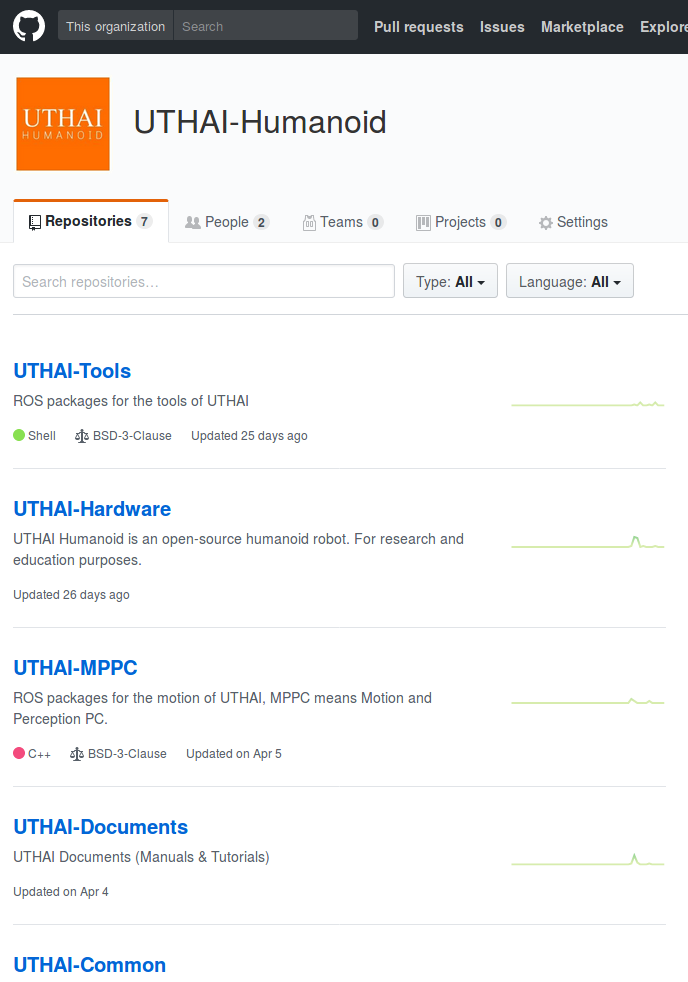
\includegraphics[width=0.42\textwidth]{chapter4/images/uthai_manual/uthai_github.png}
	\caption{GitHub ที่เก็บข้อมูลทั้งหมดของหุ่นยนต์ฮิวมานอยด์ UTHAI}
\end{figure}
\begin{figure}[!ht]
	\centering
	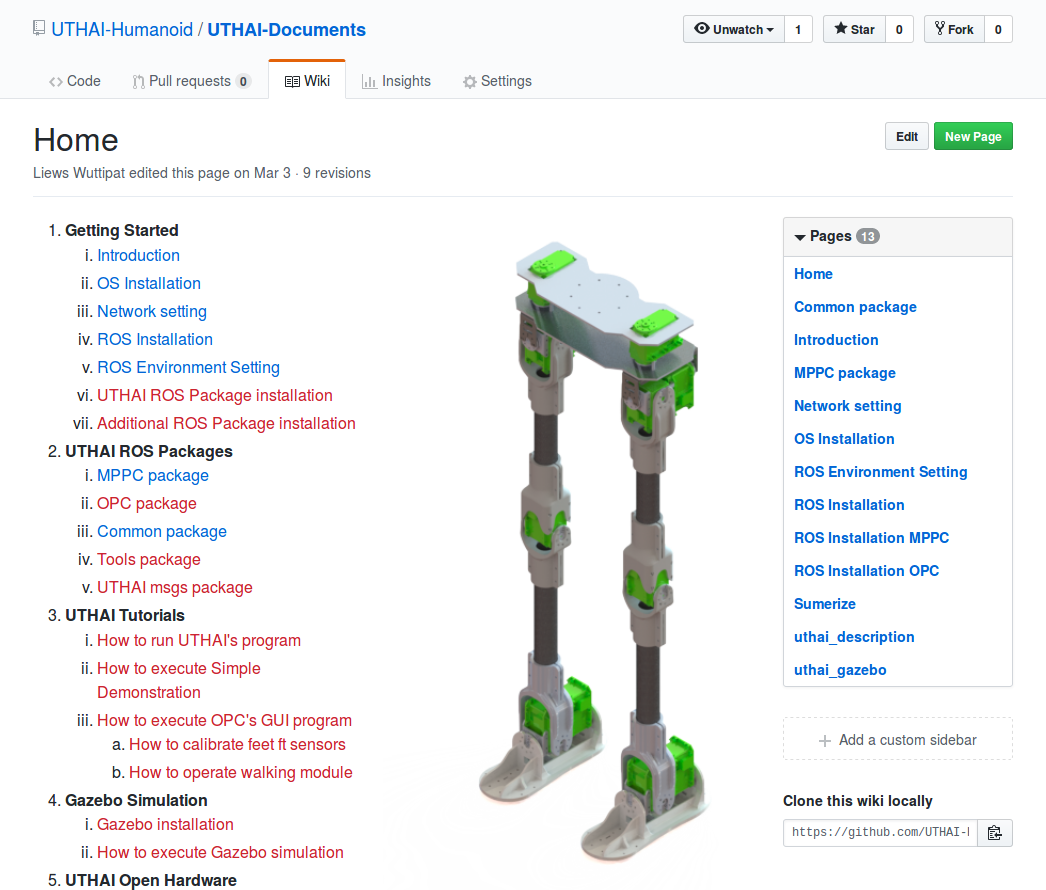
\includegraphics[width=0.60\textwidth]{chapter4/images/uthai_manual/uthai_github2.png}
	\caption{ตัวอย่าง Wiki การใช้งานเบื้องต้นของหุ่นยนต์ฮิวมานอยด์ UTHAI}
\end{figure}


\clearpage
\subsection{ตัวอย่างเฟรมของหุ่นยนต์ฮิวมานอยด์ UTHAI}
เฟรมของหุ่นยนต์ฮิวมานอยด์ UTHAIได้ถูกอัพโหลดให้อยู่บนอินเทอร์เน็ต โดยอยู่ที่ https://github.com/UTHAI-Humanoid/UTHAI-Hardware/tree/master/Mechanics/Frame

\begin{figure}[!ht]
	\centering
	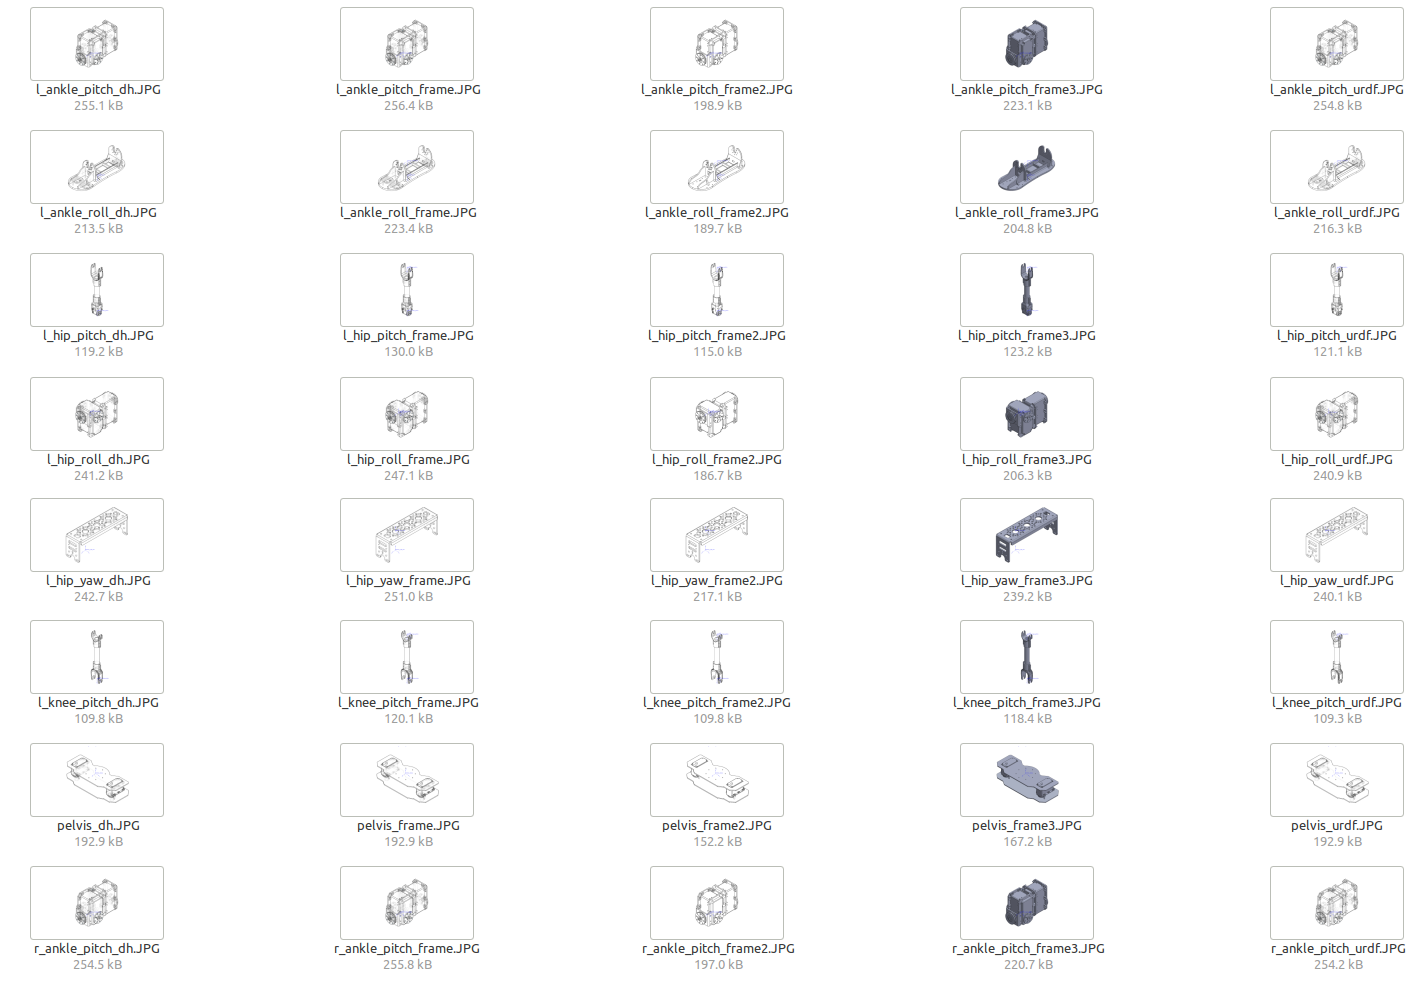
\includegraphics[width=0.85\textwidth]{chapter4/images/uthai_manual/uthai_frame.png}
	\caption{ภาพเฟรมของแต่ละพาร์ทของหุ่นยนต์ฮิวมานอยด์ UTHAI}
\end{figure}
\begin{figure}[!ht]
	\centering
	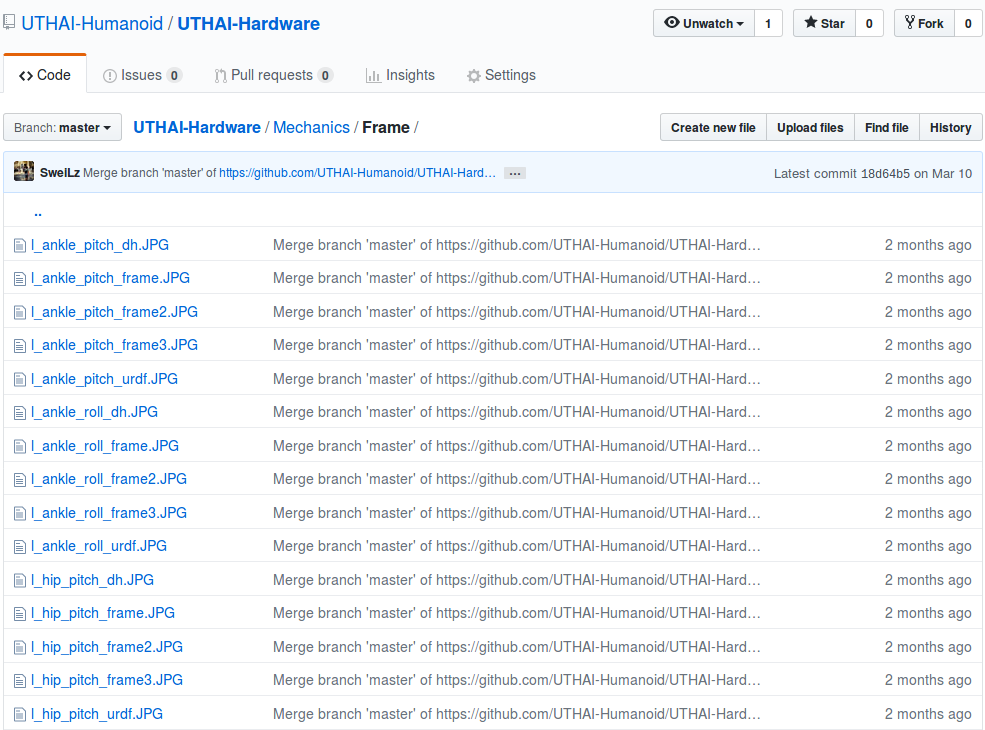
\includegraphics[width=0.85\textwidth]{chapter4/images/uthai_manual/uthai_frame2.png}
	\caption{ภาพ GitHub ของเฟรมแต่ละพาร์ทของหุ่นยนต์ฮิวมานอยด์ UTHAI}
\end{figure}

\clearpage
\subsection{ตัวอย่างเอกสารข้อมูลของหุ่นยนต์ฮิวมานอยด์ UTHAI}

\begin{figure}[!ht]
    \centering
    \begin{subfigure}[b]{0.45\textwidth}
        \centering
        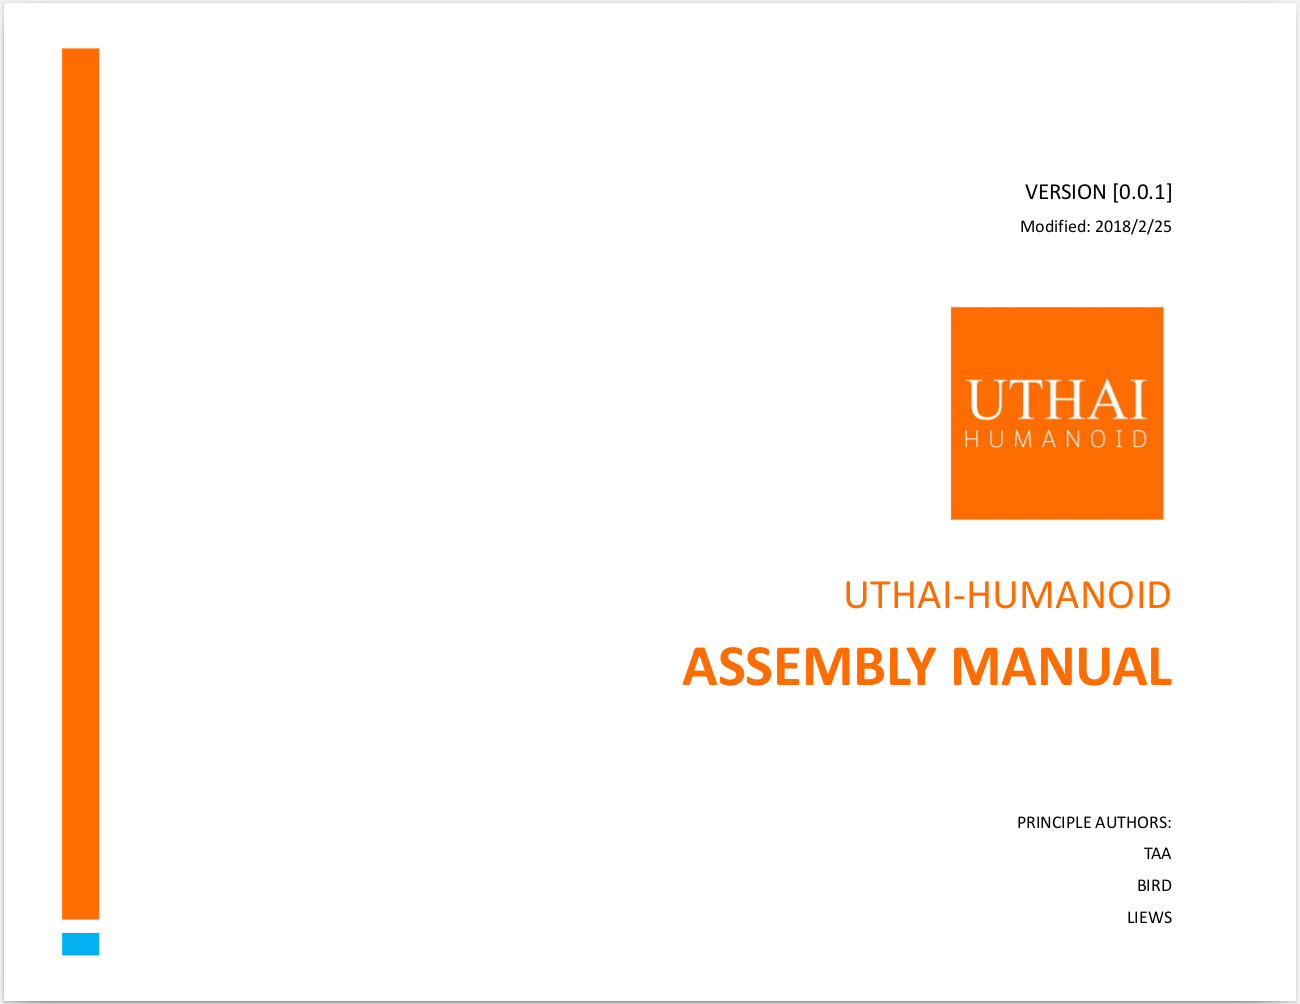
\includegraphics[width=\textwidth]{chapter4/images/uthai_manual/uthai_assembly.png}
        \caption{หน้าปกคู่มือการประกอบหุ่นยนต์ฮิวมานอยด์ UTHAI}
    \end{subfigure}
    \hfill
    \begin{subfigure}[b]{0.45\textwidth}
        \centering
        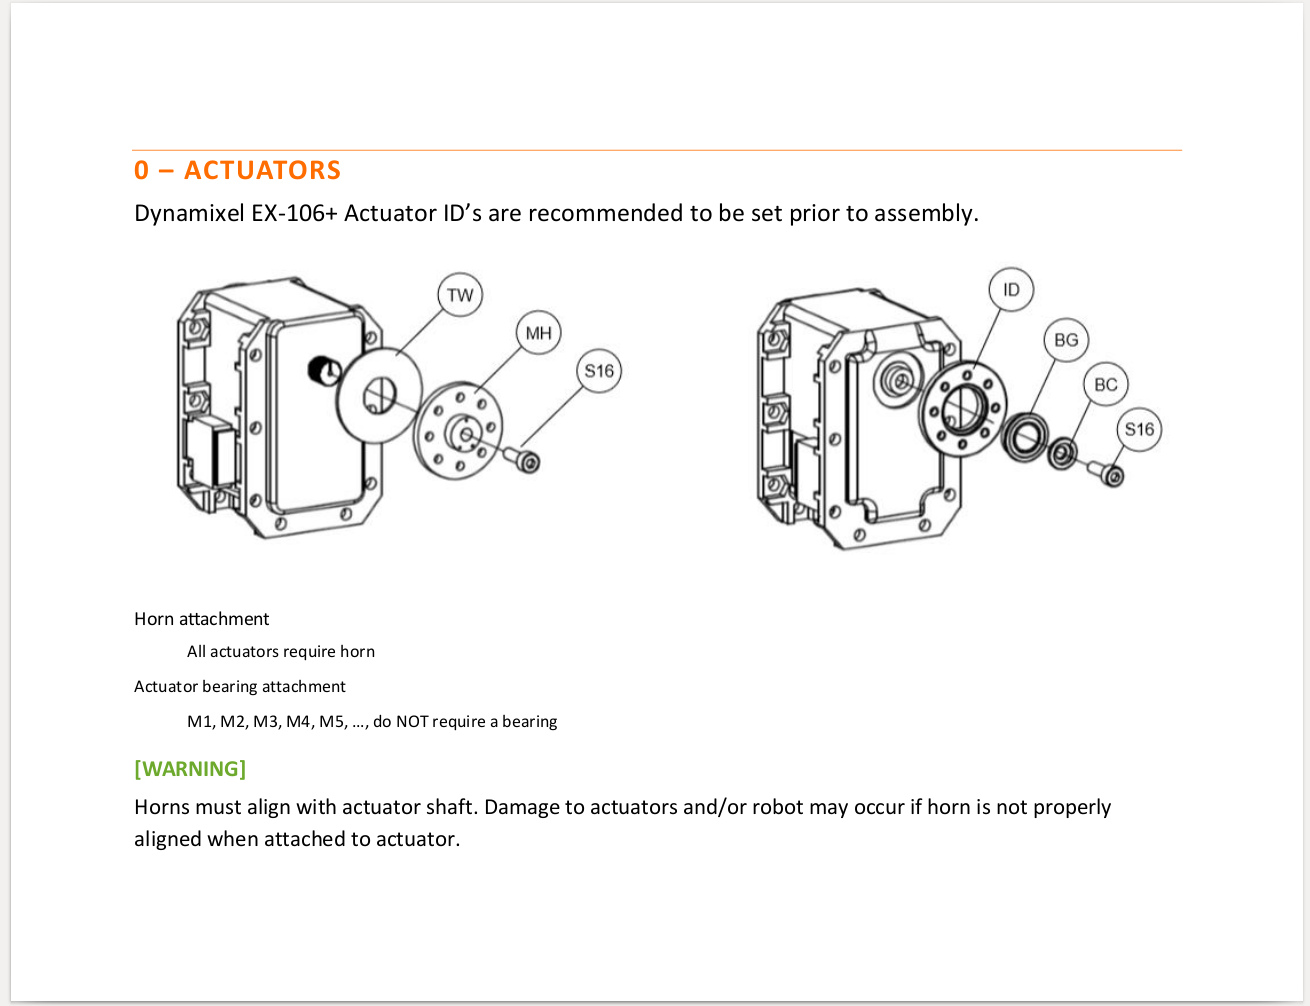
\includegraphics[width=\textwidth]{chapter4/images/uthai_manual/uthai_assembly2.png}
        \caption{ตัวอย่างคู่มือการประกอบหุ่นยนต์ฮิวมานอยด์ UTHAI}
    \end{subfigure}
    \caption{UTHAI Assembly Manual}
	\label{fig:uthai_assembly_manual}
\end{figure}
\begin{figure}[!ht]
    \centering
    \begin{subfigure}[b]{0.45\textwidth}
        \centering
        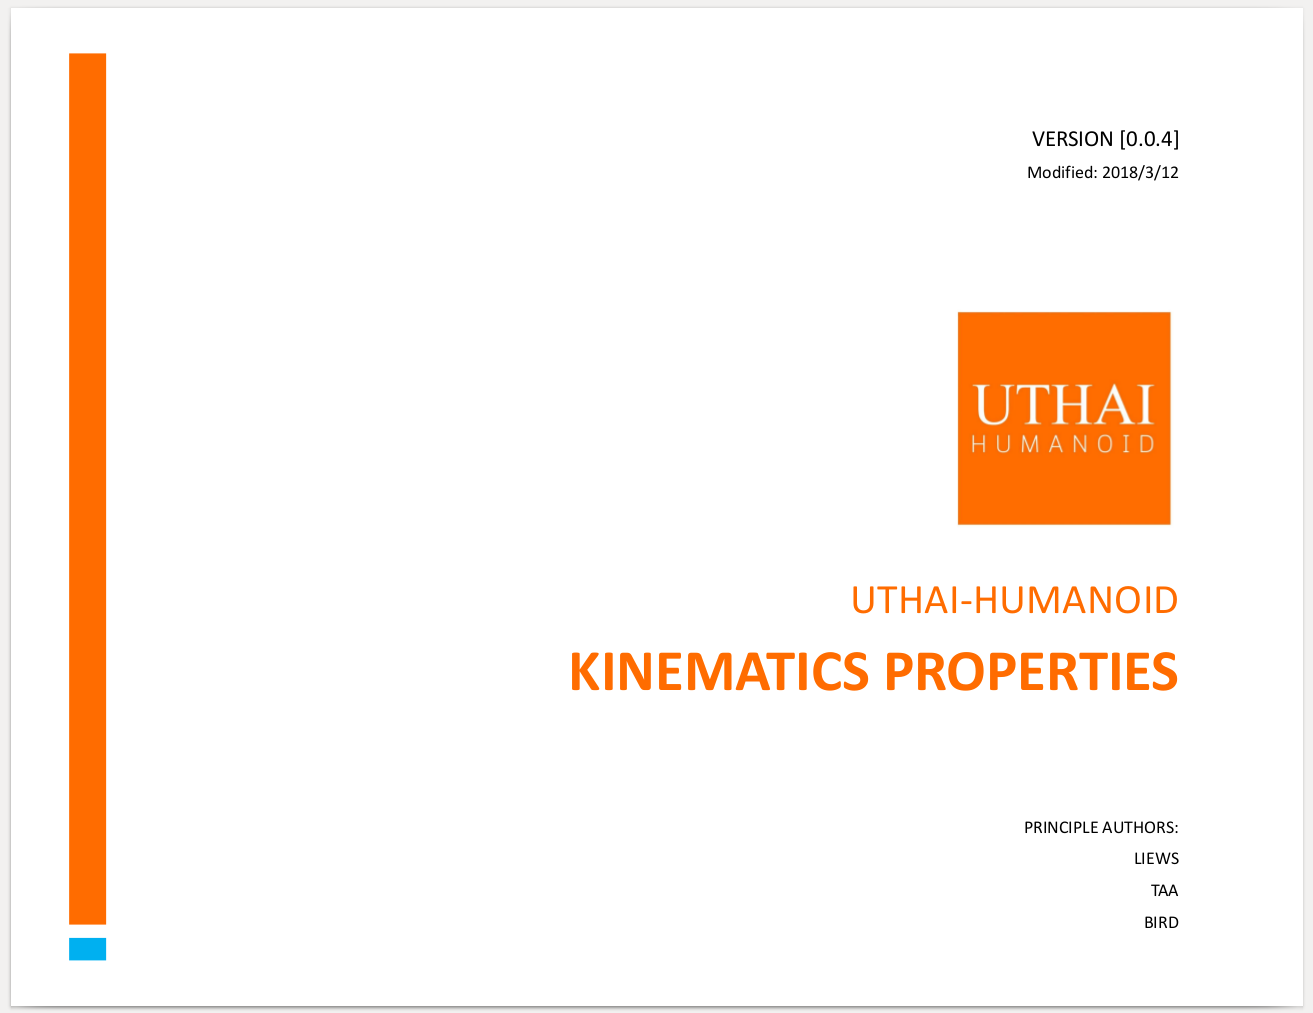
\includegraphics[width=\textwidth]{chapter4/images/uthai_manual/uthai_kinematics.png}
        \caption{หน้าปกรายละเอียดของหุ่นยนต์ฮิวมานอยด์ UTHAI}
    \end{subfigure}
    \hfill
    \begin{subfigure}[b]{0.45\textwidth}
        \centering
        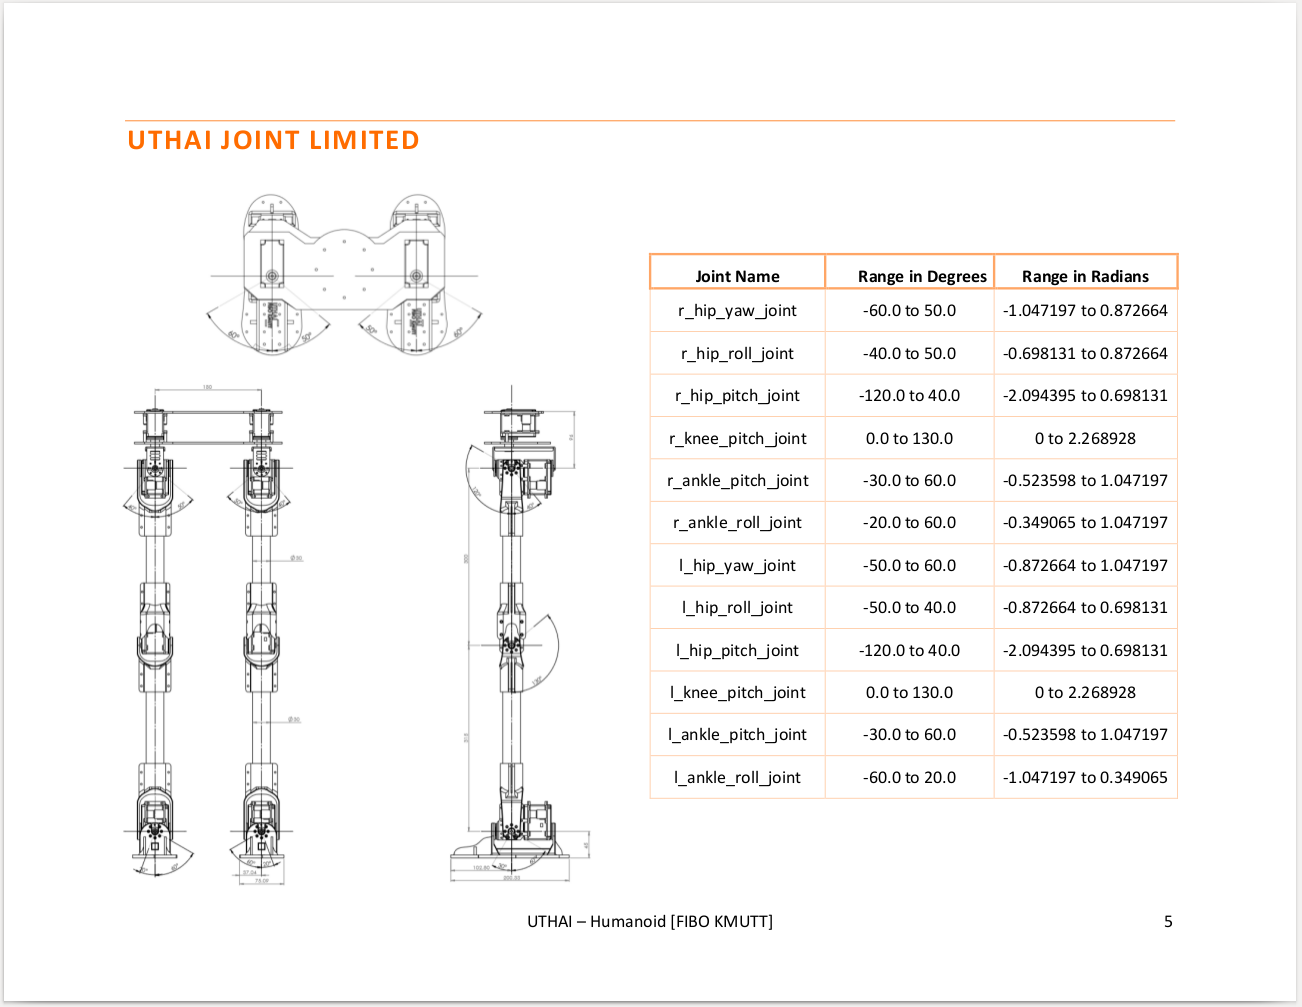
\includegraphics[width=\textwidth]{chapter4/images/uthai_manual/uthai_kinematics2.png}
        \caption{ตัวอย่างรายละเอียดของหุ่นยนต์ฮิวมานอยด์ UTHAI}
    \end{subfigure}
    \caption{UTHAI Kinematics Properties}
	\label{fig:uthai_kinematics_manual}
\end{figure}
\begin{figure}[!ht]
    \centering
    \begin{subfigure}[b]{0.45\textwidth}
        \centering
        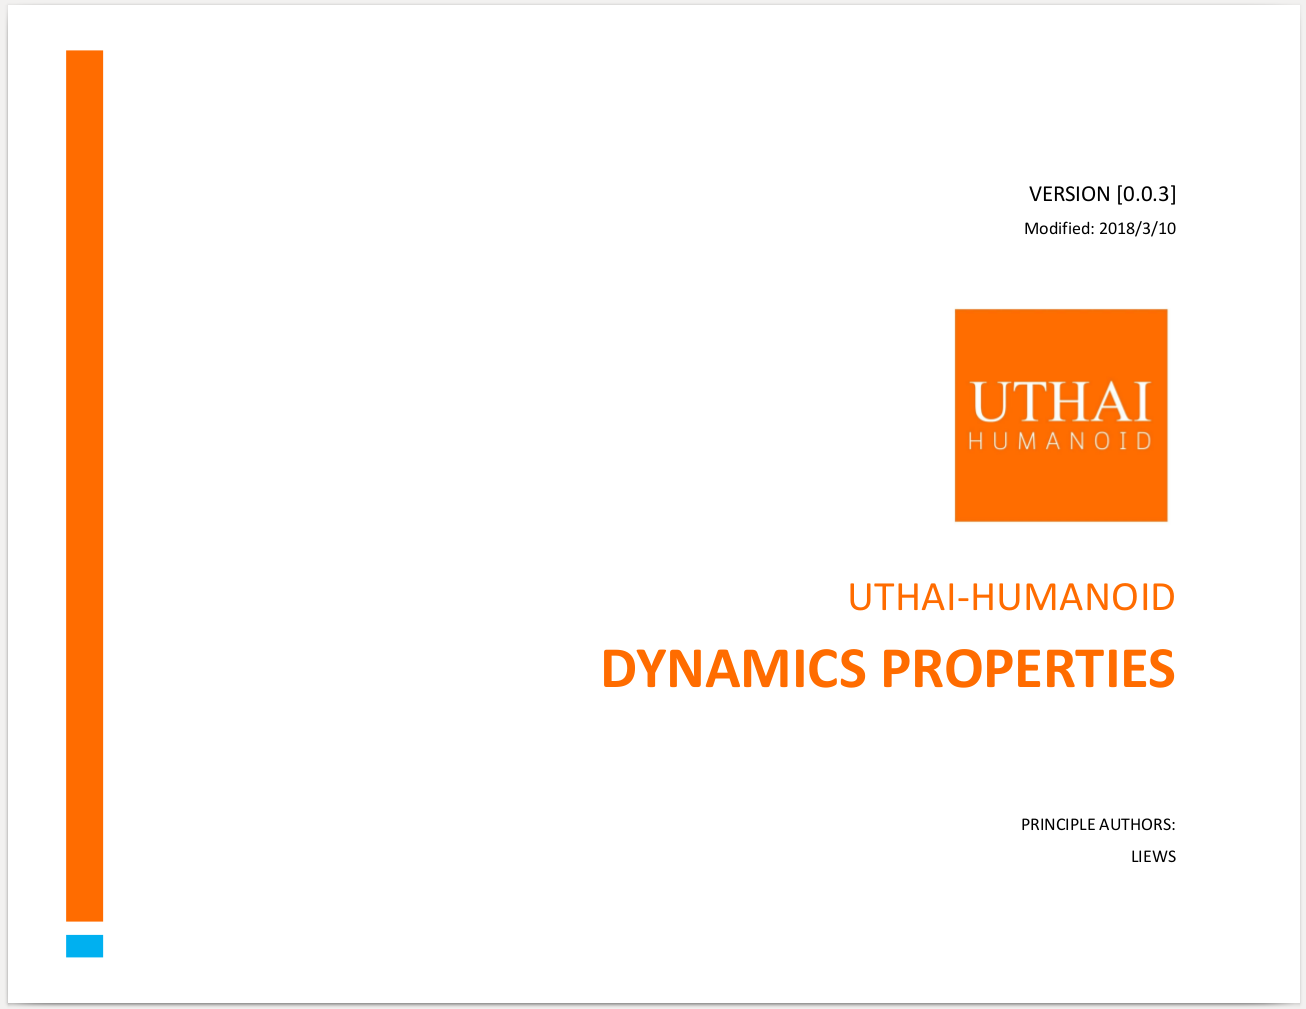
\includegraphics[width=\textwidth]{chapter4/images/uthai_manual/uthai_dynamics.png}
        \caption{หน้าปกรายละเอียดของหุ่นยนต์ฮิวมานอยด์ UTHAI}
    \end{subfigure}
    \hfill
    \begin{subfigure}[b]{0.45\textwidth}
        \centering
        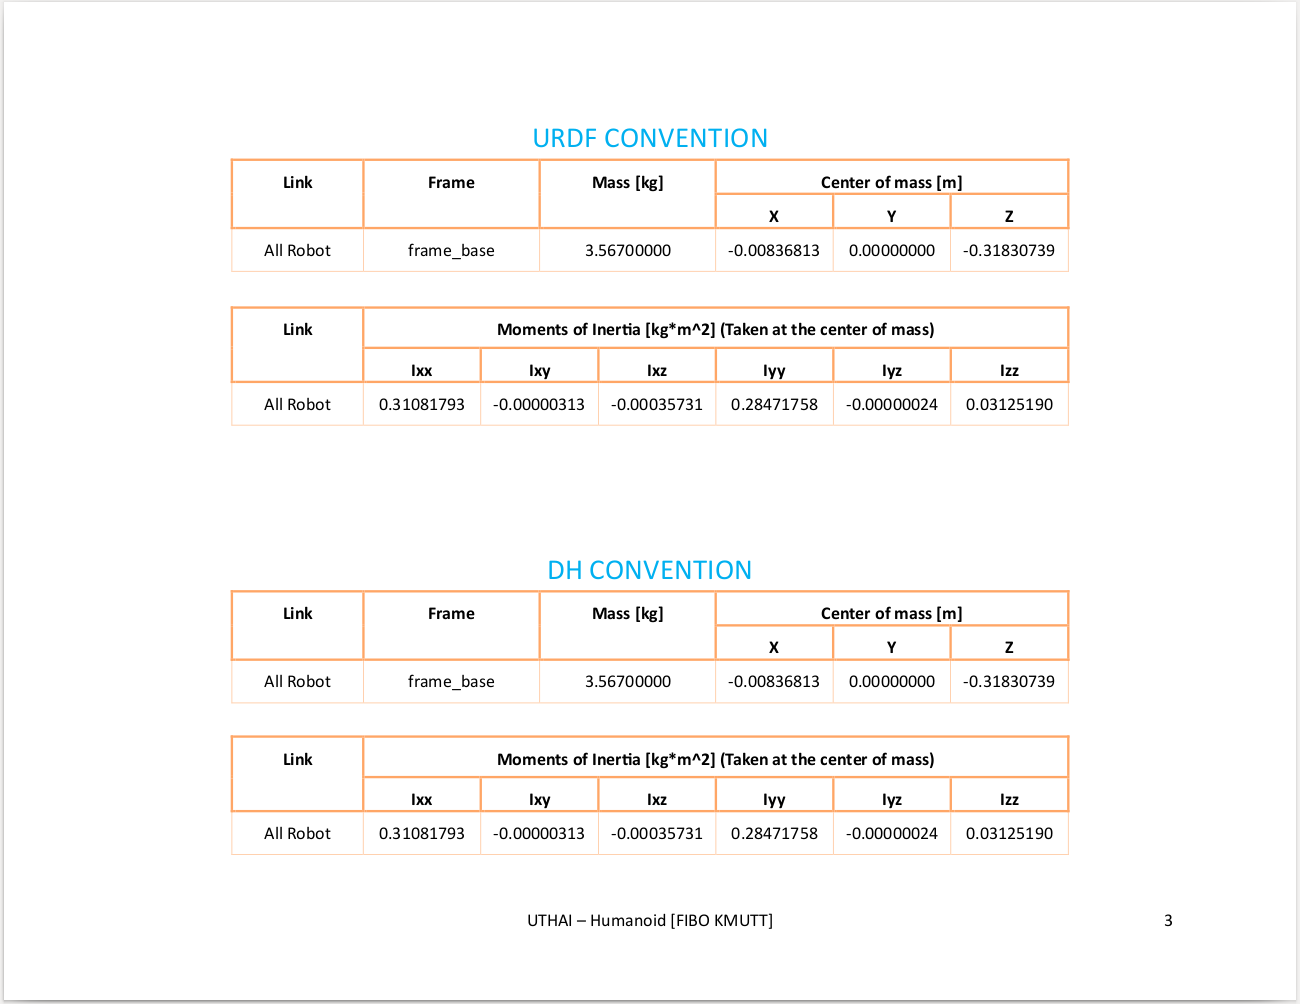
\includegraphics[width=\textwidth]{chapter4/images/uthai_manual/uthai_dynamics2.png}
        \caption{ตัวอย่างรายละเอียดของหุ่นยนต์ฮิวมานอยด์ UTHAI}
    \end{subfigure}
    \caption{UTHAI Dynamics Properties}
	\label{fig:uthai_dynamics_manual}
\end{figure}


\clearpage
\subsection{ภาพรวมระบบพื้นฐานของหุ่นยนต์ฮิวมานอยด์ UTHAI}
ระบบพื้นฐานที่ผู้วิจัยได้ทำการออกแบบก็เพื่อที่จะทำให้คนที่เข้ามาพัฒนาต่อยอดได้อย่างสะดวก และเป็นระบบระเบียบ
มีรูปแบบแบบแผน ซึ่งผู้วิจัยได้วางระบบนี้ขึ้นมาจากประสบการณ์การทำงานของผู้วิจัยเอง รวมถึงได้ค้นคว้าหาความรู้เพิ่มเติม
จนคิดว่าระบบนี้จะทำให้หุ่นยนต์ฮิวมานอยด์สามารถพัฒนาต่อได้ง่าย และเป็นประโยชน์ต่อผู้วิจัยท่านอื่นที่ต้องการนำระบบพื้นฐานนี้ไปใช้งาน

\begin{figure}[!ht]
	\centering
	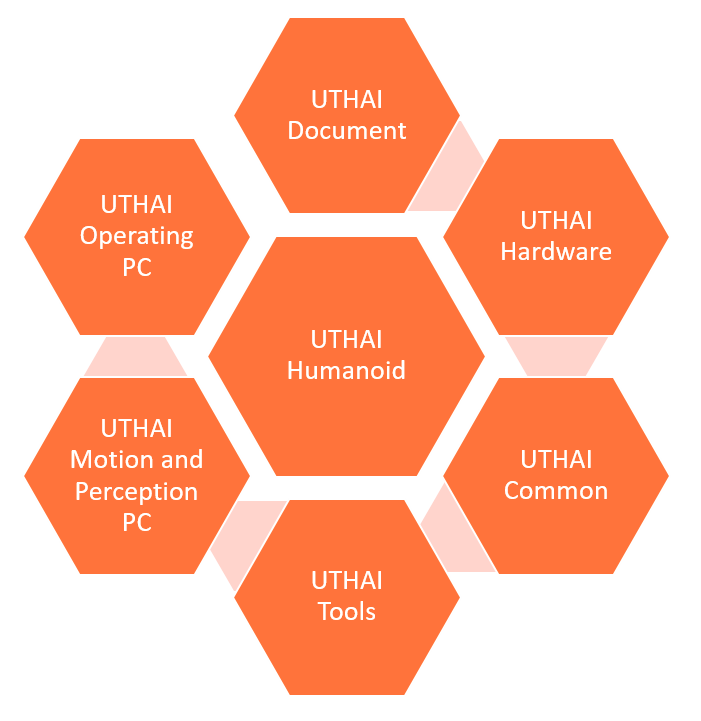
\includegraphics[width=0.7\textwidth]{chapter4/images/uthai_platform.png}
	\caption{ภาพรวมระบบพื้นฐานของหุ่นยนต์ฮิวมานอยด์ UTHAI}
	\label{fig:uthai_platform}
\end{figure}

ระบบพื้นฐานที่ผู้วิจัยออกแบบขึ้นมานั้น จะประกอบไปด้วยส่วนสำคัญอยู่ทั้งหมด 6 ส่วน คือ
\vspace{-10pt}
\begin{enumerate}[label=\arabic*., leftmargin=2.5cm]
    \setlength\itemsep{-0.25em}
    \item UTHAI-Documents
    \item UTHAI-Hardware
    \item UTHAI-Common
    \item UTHAI-MPPC
    \item UTHAI-OPC
    \item UTHAI-Tools
\end{enumerate}

\clearpage
\subsubsection*{UTHAI-Documents}
ในส่วนนี้คือส่วนของงานเอกสารต่างๆที่เกี่ยวข้องกับหุ่นยนต์ฮิวมานอยด์

\paragraph*{Reports-Hardware}
ใช้สำหรับเก็บรายงานวิทยานิพนธ์ทั้งฉบับร่างและฉบับสมบูรณ์ที่เกี่ยวข้องกับ การปรับเปลี่ยนโครงสร้างทางกล และทางไฟฟ้าของหุ่นยนต์ฮิวมานอยด์ UTHAI
\subparagraph*{- การออกแบบโครงสร้างและพัฒนาระบบพื้นฐานสำหรับหุ่นยนต์ฮิวมานอยด์เพื่อการศึกษาและวิจัย}

\paragraph*{Reports-Software}
ใช้สำหรับเก็บรายงานวิทยานิพนธ์ทั้งฉบับร่างและฉบับสมบูรณ์ที่เกี่ยวข้องกับการเพิ่มความสามารถของหุ่นยนต์ฮิวมานอยด์ UTHAI
\subparagraph*{- การพัฒนาระบบการเคลื่อนที่สำหรับหุ่นยนต์ฮิวมานอยด์}

\paragraph*{Wiki}
ใช้สำหรับเก็บ Tutorial ที่เกี่ยวกับการใช้งานของหุ่นยนต์ฮิวมานอยด์ UTHAI

\begin{figure}[!ht]
	\centering
	\includegraphics[width=0.7\textwidth]{chapter4/images/uthai_platform/uthai_doc.png}
	\caption{ภาพตัวอย่าง Tutorial ใน Wiki}
\end{figure}

ผู้วิจัยท่านอื่นสามารถที่จะช่วยกันเขียนและพัฒนาได้โดยการ Clone Repository แล้วทำการแก้ไขปรับปรุง หลังจากนั้นก็ Pull request ขึ้นมาเพื่อแสดงให้ผู้วิจัยท่านอื่นเห็นด้วย


\clearpage
\subsubsection*{UTHAI-Hardware}
ในส่วนนี้คือส่วนของรายละเอียดเกี่ยวกับโครงสร้างทั้งทางกลและทางไฟฟ้าที่เปิดให้ผู้วิจัยท่านอื่นสามารถนำไปประยุกต์ใช้ได้

\paragraph*{Drawing}
ไฟล์ออกแบบทางวิศวกรรมทุกชิ้นส่วนที่ต้องมีการขึ้นรูป
\paragraph*{STL files}
ไฟล์สำหรับการขึ้นรูปสามมิติและไฟล์สำหรับนำไปทำแบบจำลองหุ่นยนต์ฮิวมานอยด์
\paragraph*{Solidworks files}
ไฟล์ที่ออกแบบโดยใช้โปรแกรม Solidworks เพื่อให้นำไปแก้ไขปรับปรุงให้ดียิ่งขึ้นได้

\begin{figure}[!ht]
	\centering
	\includegraphics[width=0.8\textwidth]{chapter4/images/uthai_platform/uthai_hardware1.png}
	\caption{ภาพตัวอย่างไฟล์ใน UTHAI-Hardware}
\end{figure}
\begin{figure}[!ht]
	\centering
	\includegraphics[width=0.8\textwidth]{chapter4/images/uthai_platform/uthai_properties.png}
	\caption{ภาพตัวอย่างไฟล์ใน UTHAI-Hardware}
\end{figure}


\clearpage
\subsubsection*{UTHAI-Common}
ในส่วนนี้คือส่วนของแพกเกจ ROS ที่ใช้เป็นพื้นฐานสำหรับการแสดงผลด้วยภาพ และระบบจำลองโดยจะมีแบบจำลองของหุ่นยนต์ฮิวมานอยด์ UTHAI ในรูปแบบของ URDF Xacro
\paragraph*{uthai\_description}
เป็นแพกเกจที่เขียนอธิบายลักษณะของหุ่นยนต์ฮิวมานอยด์เพื่อให้ ROS สามารถนำไปใช้ในกระบวนการอื่นได้
\paragraph*{uthai\_gazebo}
เป็นแพกเกจที่เอาไว้สำหรับทำระบบจำลองการทำงานของหุ่นยนต์ฮิวมานอยด์ UTHAI

\begin{figure}[!ht]
	\centering
	\includegraphics[width=0.6\textwidth]{chapter4/images/uthai_platform/uthai_rviz.png}
	\caption{ภาพ RViz ใน uthao\_description}
\end{figure}
\begin{figure}[!ht]
	\centering
	\includegraphics[width=0.6\textwidth]{chapter4/images/uthai_platform/uthai_gazebo.png}
	\caption{ภาพ Gazebo ใน uthai\_gazebo}
\end{figure}


\clearpage
\subsubsection*{UTHAI-MPPC}
ในส่วนนี้คือส่วนของแพกเกจ ROS ที่ใช้เป็นตัวในการเชื่อมต่อกับอุปกรณ์ฮาร์ดแวร์ของหุ่นยนต์ฮิวมานอยด์ UTHAI
เพื่อสั่งการตัวขับเคลื่อนดิจิตอลเซอร์โว และอ่านค่าเซนเซอร์จากตัวรับรู้หน่วยวัดความเฉื่อย การตรวจจับฝ่าเท้า
ตำแหน่งและความเร็วของตัวขับเคลื่อน
\paragraph*{uthai\_mbed}
เป็นแพกเกจที่เขียนเชื่อมต่อกับหน่วยประมวลผลระดับต่ำผ่าน rosserial เขียนด้วยภาษา python
โดยจะรับค่าเซนเซอร์หน่วยวัดความเฉื่อย เซนเซอร์ตรวจจับพื้น
\paragraph*{uthai\_manager}
เป็นแพกเกจที่เขียนเพื่อเอาไว้สำหรับจัดการตัวขับเคลื่อนทั้งหมด ให้สามารถสั่งการได้รวมถึง config ต่างๆด้วย
\paragraph*{uthai\_bringup}
เป็นแพกเกจที่เขียนเพื่อใช้ในการสั่งการตัวขับเคลื่อน ดิจิตอลเซอร์โว ที่เชื่อมต่อกับตัวประมวลผลระดับสูง

\begin{figure}[!ht]
	\centering
	\includegraphics[width=0.8\textwidth]{chapter4/images/uthai_platform/ros_serial.png}
	\caption{ภาพ rqt\_graph ของ serial\_node}
\end{figure}


\subsubsection*{UTHAI-OPC}
ในส่วนนี้คือส่วนของแพกเกจ ROS ที่ใช้เป็นตัวในการเชื่อมต่อระหว่างตัวประมวลผลระดับสูงกับคอมพิวเตอร์ภายนอกเพื่อใช้ในการควบคุม
หรือการแสดงผลการทำงานที่ต้องใช้การคำนวณสูง เป็นการแบ่งเบาภาระการประมวลผลของตัวประมวลผลระดับสูง

\subsubsection*{UTHAI-Msgs}
ในส่วนนี้คือส่วนของแพกเกจ ROS ที่ใช้เป็นตัวในการเก็บ Messages ที่ใช้ในการติดต่อสื่อสารกันภายในระบบ ซึ่ง Messages ไม่เป็นมาตรฐาน
โดยอาจรวมไปถึง services และ actions ของระบบหุ่นยนต์ฮิวมานอยด์ UTHAIด้วย

\clearpage
\subsubsection*{UTHAI-Tools}
ในส่วนนี้คือส่วนของรายละเอียดเเครื่องมือที่ช่วยทำให้การทำงานมีประสิทธิภาพมากยิ่งขึ้น

\paragraph*{sketch-lib}
เป็นเครื่องมือที่ใช้สำหรับเอาไว้วาดรูปเฟรมของหุ่นยนต์
\begin{figure}[!ht]
    \centering
    \begin{subfigure}[b]{0.45\textwidth}
        \centering
        \includegraphics[width=\textwidth]{chapter4/images/uthai_tools/basic-shapes.png}
        \caption{ภาพตัวอย่างการวาดออฟเจ็คต่างๆ}
    \end{subfigure}
    \hfill
    \begin{subfigure}[b]{0.45\textwidth}
        \centering
        \includegraphics[width=\textwidth]{chapter4/images/uthai_tools/test_robot.png}
        \caption{ภาพตัวอย่างการวาดเฟรมของแขนกล}
    \end{subfigure}
    \caption{ภาพตัวอย่างการวาดเฟรมโดยใช้เครื่องมือนี้}
\end{figure}
\begin{figure}[!ht]
	\centering
	\includegraphics[width=0.3\textwidth]{chapter4/images/uthai_tools/uthai_kinematics.png}
	\caption{ภาพตัวอย่างการวาดเฟรมของหุ่นยนต์ฮิวมานอยด์}
	\label{fig:uthai_kinematics_sk}
\end{figure}

%\clearpage
%\section{ผลการทดลอง}
%\subsection{การทดลองการเดิน}
การทดลองการเดินนั้นได้ทดลองด้วยการปรับค่าข้อต่อให้เหมาะสมแก่การเดิน เพื่อทดสอบโครงสร้างที่ได้ออกแบบ
มาว่าสามารถรองรับการเดินของหุ่นยนต์ได้จริงหรือไม่ โดยค่าที่ใช้ในการปรับนั้นจะเป็นค่ามุมของมอเตอร์ส่วนต่างๆของส่วนขาทั้ง 2 ข้าง
โดยจะตั้งชื่อมอเตอร์ตามแกนของข้อต่อแต่ละส่วนโดยเริ่มจากส่วนจะโพกจะมี 3 แกนคือ hip yaw,hip roll,hip pitch ส่วนหัวเข่า 1 แกนคือ
knee pitch และส่วนข้อเท้า 2 แกนคือ ankle pitch,ankle roll โดยในขาแต่ละข้างจะแยกด้วยสัญลักษณ์ Right(ขาข้างขวา)และ Left(ขาข้างซ้าย)
โดยอิงจากตัวของหุ่นยนต์ และสั่งงานให้ไปตามมุมต่างๆที่กำหนดไว้ดังภาพ 

\subsubsection*{รูปกราฟแสดงตำแหน่งมอเตอร์ขาขวา}
\begin{figure}[!ht]
  \centering
  \includegraphics[width=1.0\linewidth]{chapter4/images/right_hip_roll.png}
  \caption{รูปการสั่งงานข้อต่อ right hip roll}
  \label{fig:right_hip_roll}
\end{figure}
\clearpage

\begin{figure}[!ht]
  \centering
  \includegraphics[width=1.0\linewidth]{chapter4/images/right_hip_pitch.png}
  \caption{รูปการสั่งงานข้อต่อ right hip pitch}
  \label{fig:right_hip_pitch}
\end{figure}

\begin{figure}[!ht]
  \centering
  \includegraphics[width=1.0\linewidth]{chapter4/images/right_hip_yaw.png}
  \caption{รูปการสั่งงานข้อต่อ right hip yaw}
  \label{fig:right_hip_yaw}
\end{figure}
\clearpage

\begin{figure}[!ht]
  \centering
  \includegraphics[width=1.0\linewidth]{chapter4/images/right_knee_pitch.png}
  \caption{รูปการสั่งงานข้อต่อ right knee pitch}
  \label{fig:right_knee_pitch}
\end{figure}

\begin{figure}[!ht]
  \centering
  \includegraphics[width=1.0\linewidth]{chapter4/images/right_ankle_pitch.png}
  \caption{รูปการสั่งงานข้อต่อ right ankle pitch}
  \label{fig:right_ankle_pitch}
\end{figure}
\clearpage

\begin{figure}[!ht]
  \centering
  \includegraphics[width=1.0\linewidth]{chapter4/images/right_ankle_roll.png}
  \caption{รูปการสั่งงานข้อต่อ right ankle roll}
  \label{fig:right_ankle_roll}
\end{figure} 
\clearpage
  
\subsubsection*{รูปกราฟแสดงตำแหน่งมอเตอร์ขาซ้าย}
\begin{figure}[!ht]
  \centering
  \includegraphics[width=1.0\linewidth]{chapter4/images/left_hip_roll.png}
  \caption{รูปการสั่งงานข้อต่อ left hip roll}
  \label{fig:left_hip_roll}
\end{figure}

\begin{figure}[!ht]
  \centering
  \includegraphics[width=1.0\linewidth]{chapter4/images/left_hip_pitch.png}
  \caption{รูปการสั่งงานข้อต่อ left hip pitch}
  \label{fig:left_hip_pitch}
\end{figure}
\clearpage

\begin{figure}[!ht]
  \centering
  \includegraphics[width=1.0\linewidth]{chapter4/images/left_hip_yaw.png}
  \caption{รูปการสั่งงานข้อต่อ left hip yaw}
  \label{fig:left_hip_yaw}
\end{figure}

\begin{figure}[!ht]
  \centering
  \includegraphics[width=1.0\linewidth]{chapter4/images/left_knee_pitch.png}
  \caption{รูปการสั่งงานข้อต่อ left knee pitch}
  \label{fig:left_knee_pitch}
\end{figure}
\clearpage

\begin{figure}[!ht]
  \centering
  \includegraphics[width=1.0\linewidth]{chapter4/images/left_ankle_pitch.png}
  \caption{รูปการสั่งงานข้อต่อ left ankle pitch}
  \label{fig:left_ankle_pitch}
\end{figure}

\begin{figure}[!ht]
  \centering
  \includegraphics[width=1.0\linewidth]{chapter4/images/left_ankle_roll.png}
  \caption{รูปการสั่งงานข้อต่อ left ankle roll}
  \label{fig:left_ankle_roll}
\end{figure} 
\clearpage

จากกราฟที่แสดงข้างต้นนั้นแสดงถึงตำแหน่งที่สั่งงานให้หุ่นยนต์ขยับในองศาต่างๆของข้อต่อ โดยจะสามารถสังเกตได้จาก
จุด peak ของแต่ละกราฟซึ่งมี 7 จุดในแต่ละกราฟที่เกิดขึ้นในคาบที่ไกล้เคียงกัน โดยค่าในแกน x แสดงถึงช่วงเวลาที่สั่งงานเป็นวินาที 
และแกน y แสดงองศาของมอเตอร์ในหน่วยเรเดียล โดยในการทดลองนี้ เป็นการกำหนดค่าเพื่อทดลองให้หุ่นยนต์มีการเดินเกิดขึ้น
และทดสอบโครงสร้างขณะทำการทดลองอีกด้วย ซึ่งผลการทดลองที่ได้จะพบว่าการเดินครั้งที่ 1-4 เกิดการล้มขึ้น และหลังจากครั้งที่ 5 เป็นต้นไป
หุ่นยนต์สามารถเดินได้ 1 ก้าวจากการทดลองเปลี่ยนค่าให้เหมาะสมกับระบบ ดังแสดงในรูปภาพต่อไปนี้

\begin{figure}[!ht]
    \centering
    \begin{subfigure}[b]{0.4\linewidth}
      \includegraphics[width=\linewidth]{chapter4/images/fall1.png}
      \caption{รูปการล้มครั้งที่ 1}
    \end{subfigure}
    \begin{subfigure}[b]{0.4\linewidth}
      \includegraphics[width=\linewidth]{chapter4/images/fall2.png}
      \caption{รูปการล้มครั้งที่ 2}
    \end{subfigure}
    \begin{subfigure}[b]{0.4\linewidth}
      \includegraphics[width=\linewidth]{chapter4/images/fall3.png}
      \caption{รูปการล้มครั้งที่ 3}
    \end{subfigure}
    \begin{subfigure}[b]{0.4\linewidth}
      \includegraphics[width=\linewidth]{chapter4/images/fall4.png}
      \caption{รูปการล้มครั้งที่ 4}
    \end{subfigure}
    \begin{subfigure}[b]{0.4\linewidth}
      \includegraphics[width=\linewidth]{chapter4/images/achive1.png}
      \caption{รูปการก้าวสำเร็จ}
    \end{subfigure}
    \caption{รูปการทดลองการเดินของหุ่นยนต์ UTHAI}
    \label{fig:test_result}
  \end{figure}


\clearpage
\subsection{ปัญหาที่พบและการแก้ไข}
\subsubsection{อุณหภูมิ}
เมื่อมีการใช้งานเป็นเวลานานจะส่งผลให้มอเตอร์ส่วนสะโพกและข้อเท้ามีความร้อนสูงถึง 50 องศาเซลเซียส 
เนื่องจากมีการสั่งงานให้มอเตอร์อยู่ในตำแหน่งที่กำหนด ซึ่งเมื่อมีแรงบิดข้างนอกมาเกี่ยวข้อง จะทำให้มอเตอร์นั้น
พยายามรักษามุมของตนเองไว้ ส่งผลให้เกิดความร้อนเกิดขึ้นและ ส่งผลให้มอเตอร์อ่อนแรงลงเนื่องจากความร้อนที่เกิดขึ้น 
ในการแก้ไขปัญหานี้สามารถเพิ่มเติมส่วนของการระบายอากาศซึ่งจะส่งผลให้ตัวของหุ่นยนต์นั้นมีน้ำหนักมากขึ้น หรือ หยุดการทดลอง
ไว้สักระยะเพื่อให้มีการระบายอากาศให้อยู่ในอุณหภูมิปกติ
\subsubsection{โครงสร้าง}
เนื่องจากการยึดท่อคาร์บอนไฟเบอร์นั้นได้ทำการยึดด้วยการบีบอัดเพื่อให้เกิดแรงเสียดทางสูงแต่ว่าเมื่อมีการ สั่งงานที่มีการกระชากกล่าวคือ
มีการเคลื่อนที่ของมุมมอเตอร์ที่มีความแร็วสูง จะส่งผลให้เกิดแรงบิดตามแนวแกนซึ่งเกินแรงเสียดทานที่การยึดติดจะรับไหว จึงเกิดการบิด ของข้อต่อ
เกิดขึ้น ส่งผลให้ ส่วนของเท้ามีการบิดไปจากท่าปกติ ซึ่งสามารถแก้ไขได้โดยเพิ่มแรงยึดด้วยการเสริมแผ่นยางบางๆบริเวณหน้าสัมผัสที่ติดกับท่อคาร์บอนไฟเบอร์
เพื่อเพิ่มแรงยึดไปอีกขั้นหนึ่ง 
\subsubsection{มอเตอร์}
เนื่องจากว่าตัวหุ่นยนต์มีการใช้มอเตอร์ในการขับเคลื่อนโดยตรงกับข้อต่อ ซึ่งเป็นผลทำให้ต้องใช้มอเตอร์ที่มีแรงบิดสูง
เพื่อขับเคลื่อนให้โครงสร้างมีการขยับตัวได้ แต่เนื่องจากว่าตัวหุ่นยนต์นั้นออกแบบมาให้มีความสูงที่ระดับ 1 เมตร ซึ่งหมายถึงจะมีแรง
โมเมนต์ที่เกิดขึ้นกับข้อต่อเมื่อหุ่นยนต์มีการก้าวเท้าหรือขยับตัว เป็นผลทำให้เกิด backlash เนื่องจากว่าตัวของมอเตอร์เองไม่สามารถควบคุมตำแหน่งของตนเองให้อยู่
ในมุมที่สั้งงานไว้ได้ จึงแก้ไขปัญหาโดยการเพิ่มระยะการสั่งงานเพื่อให้ครอบคลุมช่วง blacklash เพื่อที่จะให้ไปยังมุมที่ต้องการได้ และยังเพิ่มกำลังไฟให้กับมอเตอร์
จาก 12V เป็น 14V เพื่อให้มีแรงบิดที่เพิ่มมากขึ้นกว่าเดิม ซึ่งจะส่งให้ backlash น้อยลงและสามารถคุมตำแหน่งงายขึ้น



	% % ************************** Thesis Chapter5 **********************************

\chapter{การอภิปรายผล สรุปผลงานวิจัย และข้อเสนอแนะ}

\section{การอภิปรายผล}
\subsection{เครื่องมือกำกับคุณลักษณะด้วยปัญญาประดิษฐ์}
เครื่องมือกำกับคุณลักษณะด้วยปัญญาประดิษฐ์ สามารถทำงานได้ครอบคลุมความต้องการของระบบทั้งหมด คือ สามารถตัดวิดิโอช่วงที่ไม่มีมนุษย์อยู่ออกได้ , สามารถระบุตำแหน่งของมนุษย์ได้ , สามารถสร้างชุดข้อมูลสำหรับการนำไปพัฒนาโมเดลปัญญาประดิษฐ์ได้ , สามารถนำโมเดลปัญญาประดิษฐ์มาทำงานร่วมกับมนุษย์ได้ , สามารถวิเคราะห์การกระทำของมนุษย์แต่ละคนได้ แต่สำหรับการนำไปใช้จริงในงานเกี่ยวกับการวิเคราะห์ผลวิดีโอจะมีข้อจำกัดในการใช้งาน ดังนี้
\begin{enumerate}
	\item เนื่องจากในความต้องการของระบบ ต้องการเครื่องมือสำหรับการกำกับข้อมูลที่สนใจมนุษย์เป็นศูนย์กลาง ดังนั้นเครื่องมือกำกับข้อมูลจึงมีข้อจำกัดที่สามารถกำกับได้เพียงแต่มนุษย์
	\item ใน 1 รอบการทำงาน จะสามารถนำวิดีโอเข้ามาสร้างเป็นชุดข้อมูลได้เพียงแค่วิดีโอเดียว เนื่องจาก การออกแบบหน้าต่างการทำงานและโครงสร้างของโปรแกรมถูกเขียนมาเพื่ออำนวยต่อการสร้างชุดข้อมูลชุดเดียวต่อการทำงานหนึ่งครั้ง
\end{enumerate}	

\subsection{ชุดข้อมูล}
ชุดข้อมูลจะเป็นชุดข้อมูลที่ถูกสร้างมากจากเครื่องมือกำกับคุณลักษณะด้วยปัญญาประดิษฐ์ที่ผู้วิจัยได้สร้างขึ้นมา โดยจุดประสงค์ของชุดข้อมูลเพื่อนำไปพัฒนาโมเดลปัญญาประดิษฐ์เพื่อวิเคราะห์การกระทำของมนุษย์ ซึ่งชุดข้อมูลที่ผู้วิจัยได้สร้างขึ้นมามีจำนวน 3 ชุดข้อมูล คือ 
\begin{enumerate}
	\item ชุดข้อมูล Goggle datasetV1 คือ ชุดข้อมูลที่เก็บรวบรวมการกระทำของมนุษย์ทั้ง 6 หมวดหมู่ คือ นั่ง เดิน กิน นอน เล่นโทรศัพท์ ยืน โดยชุดข้อมูลใช้สำหรับการนำไปสอนให้กับโมเดลปัญญาประดิษฐ์
	\item ชุดข้อมูล Goggle datasetV2 คือการนำชุดข้อมูล Goggle datasetV1 มาเก็บข้อมูลเพิ่มเติม และ คัดกรองข้อมูลที่ไม่จำเป็นออกเพื่อใช้สำหรับการนำไปสอนและพัฒนาให้กับโมเดลปัญญาประดิษฐ์
	\item ชุดข้อมูล All action คือ ชุดข้อมูลจากวิดีโอที่ภายในวิดีโอจะประกอบด้วยการกระทำหลากหลายการกระทำอยู่ในวิดีโอ โดยชุดข้อมูลนี้จะใช้สำหรับทดสอบโมเดลปัญญาประดิษฐ์

\end{enumerate}	
\subsection{โมเดลปัญญาประดิษฐ์}
\subsubsection{การสร้างโมเดลปัญญาประดิษฐ์ด้วยโครงสร้าง ResNet50}
\par
ในการสร้างโมเดลปัญญาประดิษฐ์ด้วยโครงสร้าง ResNet50 คุณภาพของโมเดลปัญญาประดิษฐ์ที่ได้ออกมานั้นจะมีของบางหมวดหมู่ที่ได้ค่าของการทำนายออกมาน้อย ซึ่งเป็นไปได้ว่าชุดข้อมูลที่เก็บมาใช้ในการสร้างโมเดลปัญญาประดิษฐ์มีความหลากหลายที่น้อย เพราะเนื่องจากการใช้ภาพจากวิดีโอเดียวกัน และในด้านของจำนวนชุดข้อมูลที่นำมาใช้ในการสร้างโมเดลปัญญาประดิษฐ์มีจำนวนน้อยลง เพราะต้องมีการลบข้อมูลภาพในส่วนที่ผิดพลาดออก เช่น การกำกับคำผิด หรือกรอบสี่เหลี่ยมที่ไม่เจอมนุษย์ เป็นต้น การที่ในบางหมวดหมู่ที่ท่าทางการกระทำที่คล้ายคลึงกัน หรือในส่วนของความสมดุลของหมวดหมู่ที่นำมาใช้ในการสร้างโมเดลปัญญาประดิษฐ์ที่มีจำนวนของข้อมูลในแต่ละหมวดหมู่ไม่เท่ากัน


\section{สรุปผลงานวิจัย}
\subsection{เครื่องมือกำกับคุณลักษณะด้วยปัญญาประดิษฐ์}
\begin{enumerate}
	\item เครื่องมือสามารถปรับความละเอียดในการตรวจสอบมนุษย์ในเฟรมได้ (ความถี่ในการสุ่มตัวอย่างเฟรมมาตรวจสอบ)
	\item เครื่องมือสามารถคัดกรองคีย์เฟรมที่ไม่มีมนุษย์อยู่ออกได้
	\item เครื่องมือสามารถตั้งค่า threshold, min-max ของกรอบสี่เหลี่ยม เพื่อให้ได้ผลลัพธ์ที่ตรงตามความต้องการของผู้ใช้
	\item เครื่องมือสามารถตรวจหาตำแหน่งของมนุษย์บนคีย์เฟรม และ สร้างกรอบสี่เหลี่ยมครอบมนุษย์ได้
	\item เครื่องมือสามารถปรับแก้ไขตำแหน่งและขนาดของกรอบสี่เหลี่ยม
	\item เครื่องมือสามารถสร้างชุดข้อมูลสำหรับการนำไปพัฒนาโมเดลปัญญาประดิษฐ์ได้
	\item เครื่องมือสามารถนำโมเดลปัญญาประดิษฐ์มาทำงานร่วมกับมนุษย์ได้
	\item เครื่องมือสามารถระบุหมวดหมู่ของการกระทำของกรอบสี่เหลี่ยมได้
	\item เครื่องมือสามารถสร้างผลลัพธ์ออกเป็นไฟล์ xml , csv หรือ รายงานได้
\end{enumerate}

\section{ข้อเสนอแนะ}
\subsection{เครื่องมือกำกับคุณลักษณะด้วยปัญญาประดิษฐ์}
แนวคิดในการทำงานเพิ่มเติมเพื่อทำให้เครื่องมือสามารถนำไปใช้ได้หลากหลายมากขึ้นมีดังนี้
\begin{enumerate}
	\item ในขณะนี้เครื่องมือใช้โมเดลปัญญาประดิษฐ์ YOLO เป็นตัวตรวจสอบวัตถุซึ่งมีการเขียนเงื่อนไขให้เลือกตรวจสอบโดยยึดคนเป็นหลัก  ดังนั้นหากมีการปรับเปลี่ยนเงื่อนไขของเครื่องมือจะทำให้สามารถเลือกตรวจสอบวัตถุอื่นๆได้หลากหลายมากขึ้น
	\item ในขณะนี้เครื่องมือสามารถมีรูปแบบไฟล์ที่สามารถนำเข้ามาวิเคราะห์ผลได้เพียงแค่ไฟล์วิดีโอ ซึ่งหากเครื่องมือสามารถรับรูปแบบไฟล์อื่นๆได้เพิ่มขึ้น เช่น ไฟล์รูปภาพ , โฟล์เดอร์ของรูปภาพ จะเพิ่มความยืดหยุ่นของเครื่องมือมากขึ้น
\end{enumerate}

	\nocite{*}
	\bibliographystyle{plain}
	\bibliography{pages/reference}
	\addcontentsline{toc}{chapter}{เอกสารอ้างอิง}
	\begin{appendices}
		\chapter{ตัวอย่างชุดข้อมูลที่ผู้วิจัยสร้างขึ้น}
\subsection*{ตัวอย่างชุดข้อมูลสำหรับการทดสอบโมเดลปัญญาประดิษฐ์ในการตรวจจับภาพบุคคล}
\begin{figure}[!ht]
    \centering
   \begin{subfigure}[b]{0.55\linewidth}
      \includegraphics[width=\linewidth]{appendix/images/3.jpg}
    \end{subfigure}
    \begin{subfigure}[b]{0.55\linewidth}
      \includegraphics[width=\linewidth]{appendix/images/5.jpg}
    \end{subfigure}
    \begin{subfigure}[b]{0.55\linewidth}
      \includegraphics[width=\linewidth]{appendix/images/8.jpg}
    \end{subfigure}
    \begin{subfigure}[b]{0.55\linewidth}
      \includegraphics[width=\linewidth]{appendix/images/17.jpg}
    \end{subfigure}
    \caption{ตัวอย่างชุดข้อมูลสำหรับการทดสอบโมเดลปัญญาประดิษฐ์ในการตรวจจับภาพบุคค}
    \label{fig:result_track}
  \end{figure}

\subsection*{ตัวอย่างชุดข้อมูลสำหรับการสร้างโมเดลในหมวดหมู่ การตอบรับโทรศัพท์}
\begin{figure}[!ht]
    \centering
   \begin{subfigure}[b]{0.45\linewidth}
      \includegraphics[width=\linewidth]{appendix/answer_phone/000_CXS0_D0_000038.jpg}
    \end{subfigure}
    \begin{subfigure}[b]{0.45\linewidth}
      \includegraphics[width=\linewidth]{appendix/answer_phone/000_CXS0_D0_001102.jpg}
    \end{subfigure}
    \begin{subfigure}[b]{0.45\linewidth}
      \includegraphics[width=\linewidth]{appendix/answer_phone/000_CXS0_D0_001293.jpg}
    \end{subfigure}
    \begin{subfigure}[b]{0.45\linewidth}
      \includegraphics[width=\linewidth]{appendix/answer_phone/000_CXS0_D0_001791.jpg}
    \end{subfigure}
    \begin{subfigure}[b]{0.45\linewidth}
      \includegraphics[width=\linewidth]{appendix/answer_phone/000_CXS0_D0_001792.jpg}
    \end{subfigure}
    \begin{subfigure}[b]{0.45\linewidth}
      \includegraphics[width=\linewidth]{appendix/answer_phone/000_CXS0_D0_001793.jpg}
    \end{subfigure}
    \caption{ตัวอย่างชุดข้อมูลในหมวดหมู่การตอบรับโทรศัพท์}
    \label{fig:result_track}
  \end{figure}

\clearpage
\subsection*{ตัวอย่างชุดข้อมูลสำหรับการสร้างโมเดลในหมวดหมู่ การกิน }
\begin{figure}[!ht]
    \centering
   \begin{subfigure}[b]{0.45\linewidth}
      \includegraphics[width=\linewidth]{appendix/eat/000_CXS1_D0_000455.jpg}
    \end{subfigure}
    \begin{subfigure}[b]{0.45\linewidth}
      \includegraphics[width=\linewidth]{appendix/eat/000_CXS1_D0_001035.jpg}
    \end{subfigure}
    \begin{subfigure}[b]{0.45\linewidth}
      \includegraphics[width=\linewidth]{appendix/eat/001_CXS1_D0_001176.jpg}
    \end{subfigure}
    \begin{subfigure}[b]{0.45\linewidth}
      \includegraphics[width=\linewidth]{appendix/eat/001_CXS1_D0_001318.jpg}
    \end{subfigure}
    \begin{subfigure}[b]{0.45\linewidth}
      \includegraphics[width=\linewidth]{appendix/eat/001_CXS1_D0_001110.jpg}
    \end{subfigure}
    \begin{subfigure}[b]{0.45\linewidth}
      \includegraphics[width=\linewidth]{appendix/eat/001_CXS1_D0_001397.jpg}
    \end{subfigure}
    \caption{ตัวอย่างชุดข้อมูลในหมวดหมู่การกิน}
    \label{fig:result_track}
  \end{figure}

\clearpage
\subsection*{ตัวอย่างชุดข้อมูลสำหรับการสร้างโมเดลในหมวดหมู่ การนั่ง }
\begin{figure}[!ht]
    \centering
   \begin{subfigure}[b]{0.45\linewidth}
      \includegraphics[width=\linewidth]{appendix/sit/000_CXS0_D0_003661.jpg}
    \end{subfigure}
    \begin{subfigure}[b]{0.45\linewidth}
      \includegraphics[width=\linewidth]{appendix/sit/000_CXS0_D0_006682.jpg}
    \end{subfigure}
    \begin{subfigure}[b]{0.45\linewidth}
      \includegraphics[width=\linewidth]{appendix/sit/000_CXS0_D0_005740.jpg}
    \end{subfigure}
    \begin{subfigure}[b]{0.45\linewidth}
      \includegraphics[width=\linewidth]{appendix/sit/000_CXS0_D0_006436.jpg}
    \end{subfigure}
    \begin{subfigure}[b]{0.45\linewidth}
      \includegraphics[width=\linewidth]{appendix/sit/000_CXS0_D0_005760.jpg}
    \end{subfigure}
    \begin{subfigure}[b]{0.45\linewidth}
      \includegraphics[width=\linewidth]{appendix/sit/000_CXS0_D0_006295.jpg}
    \end{subfigure}
    \caption{ตัวอย่างชุดข้อมูลในหมวดหมู่การกิน}
    \label{fig:result_track}
  \end{figure}

\clearpage
\subsection*{ตัวอย่างชุดข้อมูลสำหรับการสร้างโมเดลในหมวดหมู่ การนอน}
\begin{figure}[!ht]
    \centering
   \begin{subfigure}[b]{0.45\linewidth}
      \includegraphics[width=\linewidth]{appendix/sleep/000_CXS0_D0_000043.jpg}
    \end{subfigure}
    \begin{subfigure}[b]{0.45\linewidth}
      \includegraphics[width=\linewidth]{appendix/sleep/000_CXS0_D0_000052.jpg}
    \end{subfigure}
    \begin{subfigure}[b]{0.45\linewidth}
      \includegraphics[width=\linewidth]{appendix/sleep/000_CXS0_D0_000069.jpg}
    \end{subfigure}
    \begin{subfigure}[b]{0.45\linewidth}
      \includegraphics[width=\linewidth]{appendix/sleep/002_CXS0_D0_000782.jpg}
    \end{subfigure}
    \begin{subfigure}[b]{0.45\linewidth}
      \includegraphics[width=\linewidth]{appendix/sleep/000_CXS0_D0_000073.jpg}
    \end{subfigure}
    \begin{subfigure}[b]{0.45\linewidth}
      \includegraphics[width=\linewidth]{appendix/sleep/002_CXS0_D0_000647.jpg}
    \end{subfigure}
    \caption{ตัวอย่างชุดข้อมูลในหมวดหมู่การนอน}
    \label{fig:result_track}
  \end{figure}

\clearpage
\subsection*{ตัวอย่างชุดข้อมูลสำหรับการสร้างโมเดลในหมวดหมู่ การยืน}
\begin{figure}[!ht]
    \centering
   \begin{subfigure}[b]{0.45\linewidth}
      \includegraphics[width=\linewidth]{appendix/stand/000_CXS0_D0_001005.jpg}
    \end{subfigure}
    \begin{subfigure}[b]{0.45\linewidth}
      \includegraphics[width=\linewidth]{appendix/stand/000_CXS0_D0_001045.jpg}
    \end{subfigure}
    \begin{subfigure}[b]{0.45\linewidth}
      \includegraphics[width=\linewidth]{appendix/stand/000_CXS0_D0_001046.jpg}
    \end{subfigure}
    \begin{subfigure}[b]{0.45\linewidth}
      \includegraphics[width=\linewidth]{appendix/stand/001_CXS3_D2_000254.jpg}
    \end{subfigure}
    \begin{subfigure}[b]{0.45\linewidth}
      \includegraphics[width=\linewidth]{appendix/stand/000_CXS0_D0_000001.jpg}
    \end{subfigure}
    \begin{subfigure}[b]{0.45\linewidth}
      \includegraphics[width=\linewidth]{appendix/stand/000_CXS0_D0_000922.jpg}
    \end{subfigure}
    \caption{ตัวอย่างชุดข้อมูลในหมวดหมู่การยืน}
    \label{fig:result_track}
 \end{figure}


\clearpage
\subsection*{ตัวอย่างชุดข้อมูลสำหรับการสร้างโมเดลในหมวดหมู่ การเดิน}
\begin{figure}[!ht]
    \centering
    \begin{subfigure}[b]{0.45\linewidth}
      \includegraphics[width=\linewidth]{appendix/walk/000_CXS0_D0_000568.jpg}
    \end{subfigure}
    \begin{subfigure}[b]{0.45\linewidth}
      \includegraphics[width=\linewidth]{appendix/walk/000_CXS0_D0_0005656.jpg}
    \end{subfigure}
   \begin{subfigure}[b]{0.45\linewidth}
      \includegraphics[width=\linewidth]{appendix/walk/000_CXS0_D0_000187.jpg}
    \end{subfigure}
    \begin{subfigure}[b]{0.45\linewidth}
      \includegraphics[width=\linewidth]{appendix/walk/000_CXS0_D0_000542.jpg}
    \end{subfigure}
    \begin{subfigure}[b]{0.45\linewidth}
      \includegraphics[width=\linewidth]{appendix/walk/000_CXS0_D0_000900.jpg}
    \end{subfigure}
    \begin{subfigure}[b]{0.45\linewidth}
      \includegraphics[width=\linewidth]{appendix/walk/000_CXS0_D0_000963.jpg}
    \end{subfigure}
    \caption{ตัวอย่างชุดข้อมูลในหมวดหมู่การยืน}
    \label{fig:result_track}
 \end{figure}

\clearpage
\subsection*{ตัวอย่างชุดข้อมูลสำหรับการสร้างโมเดลในหมวดหมู่รูปภาพทีเกิดข้อผิดพลาด}
รูปภาพที่เราคัดกรองออกเนื่องจากกกรณ๊พิเศษดังนี้ 1.มีบุคคลอยู่ไม่เต็มรูปภาพ 2.มีคนมากกว่า 1 คน ภายในรูปภาพ 3.รูปภาพมืดหรือไม่ชัด
\begin{figure}[!ht]
    \centering
    \begin{subfigure}[b]{0.45\linewidth}
      \includegraphics[width=\linewidth]{appendix/unknown/000_CXS0_D0_000149.jpg}
    \end{subfigure}
   \begin{subfigure}[b]{0.45\linewidth}
      \includegraphics[width=\linewidth]{appendix/unknown/000_CXS0_D0_001793.jpg}
    \end{subfigure}
    \begin{subfigure}[b]{0.45\linewidth}
      \includegraphics[width=\linewidth]{appendix/unknown/000_CXS0_D0_001794.jpg}
    \end{subfigure}
    \begin{subfigure}[b]{0.45\linewidth}
      \includegraphics[width=\linewidth]{appendix/unknown/001_CXS2_D1_001979.jpg}
    \end{subfigure}
    \caption{ตัวอย่างชุดข้อมูลในหมวดหมู่รูปภาพทีเกิดข้อผิดพลาด}
    \label{fig:result_track}
 \end{figure}



		% \chapter{แหล่งข้อมูล Latex}
\section{แหล่งข้อมูลออนไลน์}


	\end{appendices}

	% \clearpage

\chapter*{ประวัติผู้เขียน}
\addcontentsline{toc}{chapter}{ประวัติผู้เขียน}
\section*{นายจิรัฏฐ์ ศรีรัตนอาภรณ์}

\hrule height .7pt
\begin{figure}[!ht]
	\centering
	\includegraphics[width=0.4\textwidth]{pages/images/jirad.jpg}
\end{figure}
\hrule height .7pt
\raggedright
\begin{tabular}{p{.25\textwidth} p{.65\textwidth}}
    \textbf{ชื่อ สกุล} & {นายจิรัฏฐ์ ศรีรัตนอาภรณ์} \\
    \textbf{รหัสนักศึกษา} & {57340500067}\\
    \textbf{วุฒิการศึกษา} & {วิศวกรรมศาสตรบัณฑิต} \\
    {} & {วิศวกรรมหุนยนตและระบบอัตโนมัติ}\\
    \textbf{ชื่อสถาบัน} & {มหาวิทยาลัยเทคโนโลยีพระจอมเกลาธนบุรี} \\
    \textbf{ปีที่สำเร็จการศึกษา} & {2560} \\
    % \textbf{ทุนการศึกษา} & {กินกันตายเทค}\\
    % {} & {กิดาฟนนนนหกดาา}\\
\end{tabular}   

\chapter*{ประวัติผู้เขียน}
\section*{นายเจษฎากร ทาไชยวงค์}
\hrule height .7pt
\begin{figure}[!ht]
	\centering
	\includegraphics[width=0.4\textwidth]{pages/images/taa.jpg}
\end{figure}
\hrule height .7pt
\raggedright
\begin{tabular}{p{.25\textwidth} p{.65\textwidth}}
    \textbf{ชื่อ สกุล} & {นายเจษฎากร ทาไชยวงค์} \\
    \textbf{รหัสนักศึกษา} & {57340500067}\\
    \textbf{วุฒิการศึกษา} & {วิศวกรรมศาสตรบัณฑิต} \\
    {} & {วิศวกรรมหุนยนตและระบบอัตโนมัติ}\\
    \textbf{ชื่อสถาบัน} & {มหาวิทยาลัยเทคโนโลยีพระจอมเกลาธนบุรี} \\
    \textbf{ปีที่สำเร็จการศึกษา} & {2560} \\
\end{tabular}   

\chapter*{ประวัติผู้เขียน}
\section*{นายวุฒิภัทร โชคอนันตทรัพย์}
\hrule height .7pt
\begin{figure}[!ht]
	\centering
	\includegraphics[width=0.65\textwidth]{pages/images/wuttipat.jpg}
\end{figure}
\hrule height .7pt
\raggedright
\begin{tabular}{p{.25\textwidth} p{.60\textwidth}}
    \textbf{ชื่อ สกุล} & {นายวุฒิภัทร โชคอนันตทรัพย์} \\
    \textbf{รหัสนักศึกษา} & {57340500067}\\
    \textbf{วุฒิการศึกษา} & {วิศวกรรมศาสตรบัณฑิต} \\
    {} & {วิศวกรรมหุนยนตและระบบอัตโนมัติ}\\
    \textbf{ชื่อสถาบัน} & {มหาวิทยาลัยเทคโนโลยีพระจอมเกลาธนบุรี} \\
    \textbf{ปีที่สำเร็จการศึกษา} & {2560} \\
    % \textbf{ทุนการศึกษา} & {กินกันตายเทค}\\
    % {} & {กิดาฟนนนนหกดาา}\\
\end{tabular}   

% \chapter*{ประวัติอาจารย์ที่ปรึกษา}
% \section*{นายธนัชชา ชูพจน์เจริญ}
% \hrule height .7pt
% \begin{figure}[!ht]
% 	\centering
% 	\includegraphics[width=0.65\textwidth]{pages/images/wuttipat.jpg}
% \end{figure}
% \hrule height .7pt
% \raggedright
% \begin{tabular}{p{.25\textwidth} p{.60\textwidth}}
%     \textbf{ชื่อ สกุล} & {นายธนัชชา ชูพจน์เจริญ} \\
%     % \textbf{วุฒิการศึกษา} & {วิศวกรรมศาสตรบัณฑิต} \\
%     % {} & {วิศวกรรมหุนยนตและระบบอัตโนมัติ}\\
%     \textbf{ชื่อสถาบัน} & {มหาวิทยาลัยเทคโนโลยีพระจอมเกลาธนบุรี} \\
%     \textbf{ปีที่สำเร็จการศึกษา} & {2560} \\
% \end{tabular}   

\end{document}